\documentclass[twoside]{book}

% Packages required by doxygen
\usepackage{calc}
\usepackage{doxygen}
\usepackage{graphicx}
\usepackage[utf8]{inputenc}
\usepackage{makeidx}
\usepackage{multicol}
\usepackage{multirow}
\usepackage{textcomp}
\usepackage[table]{xcolor}

% Font selection
\usepackage[T1]{fontenc}
\usepackage{mathptmx}
\usepackage[scaled=.90]{helvet}
\usepackage{courier}
\usepackage{amssymb}
\usepackage{sectsty}
\renewcommand{\familydefault}{\sfdefault}
\allsectionsfont{%
  \fontseries{bc}\selectfont%
  \color{darkgray}%
}
\renewcommand{\DoxyLabelFont}{%
  \fontseries{bc}\selectfont%
  \color{darkgray}%
}

% Page & text layout
\usepackage{geometry}
\geometry{%
  a4paper,%
  top=2.5cm,%
  bottom=2.5cm,%
  left=2.5cm,%
  right=2.5cm%
}
\tolerance=750
\hfuzz=15pt
\hbadness=750
\setlength{\emergencystretch}{15pt}
\setlength{\parindent}{0cm}
\setlength{\parskip}{0.2cm}
\makeatletter
\renewcommand{\paragraph}{%
  \@startsection{paragraph}{4}{0ex}{-1.0ex}{1.0ex}{%
    \normalfont\normalsize\bfseries\SS@parafont%
  }%
}
\renewcommand{\subparagraph}{%
  \@startsection{subparagraph}{5}{0ex}{-1.0ex}{1.0ex}{%
    \normalfont\normalsize\bfseries\SS@subparafont%
  }%
}
\makeatother

% Headers & footers
\usepackage{fancyhdr}
\pagestyle{fancyplain}
\fancyhead[LE]{\fancyplain{}{\bfseries\thepage}}
\fancyhead[CE]{\fancyplain{}{}}
\fancyhead[RE]{\fancyplain{}{\bfseries\leftmark}}
\fancyhead[LO]{\fancyplain{}{\bfseries\rightmark}}
\fancyhead[CO]{\fancyplain{}{}}
\fancyhead[RO]{\fancyplain{}{\bfseries\thepage}}
\fancyfoot[LE]{\fancyplain{}{}}
\fancyfoot[CE]{\fancyplain{}{}}
\fancyfoot[RE]{\fancyplain{}{\bfseries\scriptsize Generated on Mon Nov 16 2015 21\-:03\-:44 for Chaos\-Core  $\vert$  A\-P\-I by Doxygen }}
\fancyfoot[LO]{\fancyplain{}{\bfseries\scriptsize Generated on Mon Nov 16 2015 21\-:03\-:44 for Chaos\-Core  $\vert$  A\-P\-I by Doxygen }}
\fancyfoot[CO]{\fancyplain{}{}}
\fancyfoot[RO]{\fancyplain{}{}}
\renewcommand{\footrulewidth}{0.4pt}
\renewcommand{\chaptermark}[1]{%
  \markboth{#1}{}%
}
\renewcommand{\sectionmark}[1]{%
  \markright{\thesection\ #1}%
}

% Indices & bibliography
\usepackage{natbib}
\usepackage[titles]{tocloft}
\setcounter{tocdepth}{3}
\setcounter{secnumdepth}{5}
\makeindex

% Hyperlinks (required, but should be loaded last)
\usepackage{ifpdf}
\ifpdf
  \usepackage[pdftex,pagebackref=true]{hyperref}
\else
  \usepackage[ps2pdf,pagebackref=true]{hyperref}
\fi
\hypersetup{%
  colorlinks=true,%
  linkcolor=blue,%
  citecolor=blue,%
  unicode%
}

% Custom commands
\newcommand{\clearemptydoublepage}{%
  \newpage{\pagestyle{empty}\cleardoublepage}%
}


%===== C O N T E N T S =====

\begin{document}

% Titlepage & ToC
\hypersetup{pageanchor=false}
\pagenumbering{roman}
\begin{titlepage}
\vspace*{7cm}
\begin{center}%
{\Large Chaos\-Core $\vert$ A\-P\-I \\[1ex]\large Version 0.\-0.\-1 }\\
\vspace*{1cm}
{\large Generated by Doxygen 1.8.6}\\
\vspace*{0.5cm}
{\small Mon Nov 16 2015 21:03:44}\\
\end{center}
\end{titlepage}
\clearemptydoublepage
\tableofcontents
\clearemptydoublepage
\pagenumbering{arabic}
\hypersetup{pageanchor=true}

%--- Begin generated contents ---
\chapter{Chaos\-Core C++ Documentation}
\label{index}\hypertarget{index}{}Chaos\+Core is generic library that provides useful data types and functions. 
\chapter{Namespace Index}
\section{Namespace List}
Here is a list of all documented namespaces with brief descriptions\+:\begin{DoxyCompactList}
\item\contentsline{section}{\hyperlink{namespacechaos}{chaos} \\*Global Chaos\+Core namespace which contains everything within Chaos\+Core }{\pageref{namespacechaos}}{}
\item\contentsline{section}{\hyperlink{namespacechaos_1_1base}{chaos\+::base} \\*Contains the base components of Chaos\+Core }{\pageref{namespacechaos_1_1base}}{}
\item\contentsline{section}{\hyperlink{namespacechaos_1_1base_1_1str}{chaos\+::base\+::str} \\*String related classes and operations }{\pageref{namespacechaos_1_1base_1_1str}}{}
\end{DoxyCompactList}

\chapter{Hierarchical Index}
\section{Class Hierarchy}
This inheritance list is sorted roughly, but not completely, alphabetically\+:\begin{DoxyCompactList}
\item exception\begin{DoxyCompactList}
\item \contentsline{section}{chaos\+:\+:ex\+:\+:Chaos\+Exception}{\pageref{classchaos_1_1ex_1_1_chaos_exception}}{}
\begin{DoxyCompactList}
\item \contentsline{section}{chaos\+:\+:ex\+:\+:Conversion\+Data\+Error}{\pageref{classchaos_1_1ex_1_1_conversion_data_error}}{}
\item \contentsline{section}{chaos\+:\+:ex\+:\+:Index\+Out\+Of\+Bounds\+Error}{\pageref{classchaos_1_1ex_1_1_index_out_of_bounds_error}}{}
\item \contentsline{section}{chaos\+:\+:ex\+:\+:Value\+Error}{\pageref{classchaos_1_1ex_1_1_value_error}}{}
\item \contentsline{section}{chaos\+:\+:io\+:\+:file\+:\+:ex\+:\+:File\+System\+Error}{\pageref{classchaos_1_1io_1_1file_1_1ex_1_1_file_system_error}}{}
\begin{DoxyCompactList}
\item \contentsline{section}{chaos\+:\+:io\+:\+:file\+:\+:ex\+:\+:Ambiguous\+Path\+Error}{\pageref{classchaos_1_1io_1_1file_1_1ex_1_1_ambiguous_path_error}}{}
\item \contentsline{section}{chaos\+:\+:io\+:\+:file\+:\+:ex\+:\+:Create\+Directory\+Error}{\pageref{classchaos_1_1io_1_1file_1_1ex_1_1_create_directory_error}}{}
\end{DoxyCompactList}
\end{DoxyCompactList}
\end{DoxyCompactList}
\item \contentsline{section}{chaos\+:\+:test\+:\+:Fixture}{\pageref{classchaos_1_1test_1_1_fixture}}{}
\item \contentsline{section}{chaos\+:\+:io\+:\+:file\+:\+:Path}{\pageref{classchaos_1_1io_1_1file_1_1_path}}{}
\item \contentsline{section}{chaos\+:\+:str\+:\+:U\+T\+F8\+String}{\pageref{classchaos_1_1str_1_1_u_t_f8_string}}{}
\end{DoxyCompactList}

\chapter{Class Index}
\section{Class List}
Here are the classes, structs, unions and interfaces with brief descriptions\-:\begin{DoxyCompactList}
\item\contentsline{section}{\hyperlink{classchaos_1_1io_1_1file_1_1ex_1_1_ambiguous_path_error}{chaos\-::io\-::file\-::ex\-::\-Ambiguous\-Path\-Error} \\*Warns that has a request has been made to create a file or directory that results in a ambiguous file system path }{\pageref{classchaos_1_1io_1_1file_1_1ex_1_1_ambiguous_path_error}}{}
\item\contentsline{section}{\hyperlink{classchaos_1_1ex_1_1_chaos_exception}{chaos\-::ex\-::\-Chaos\-Exception} \\*Abstract base class that all Chaos\-Core Exceptions extend from }{\pageref{classchaos_1_1ex_1_1_chaos_exception}}{}
\item\contentsline{section}{\hyperlink{classchaos_1_1ex_1_1_conversion_data_error}{chaos\-::ex\-::\-Conversion\-Data\-Error} \\*Warns that the provided data for a type conversion was bad or invalid }{\pageref{classchaos_1_1ex_1_1_conversion_data_error}}{}
\item\contentsline{section}{\hyperlink{classchaos_1_1io_1_1file_1_1ex_1_1_create_directory_error}{chaos\-::io\-::file\-::ex\-::\-Create\-Directory\-Error} \\*Warns that creating a directory has failed }{\pageref{classchaos_1_1io_1_1file_1_1ex_1_1_create_directory_error}}{}
\item\contentsline{section}{\hyperlink{classchaos_1_1io_1_1file_1_1ex_1_1_file_system_error}{chaos\-::io\-::file\-::ex\-::\-File\-System\-Error} \\*A generic error relating to the file system }{\pageref{classchaos_1_1io_1_1file_1_1ex_1_1_file_system_error}}{}
\item\contentsline{section}{\hyperlink{classchaos_1_1test_1_1_fixture}{chaos\-::test\-::\-Fixture} \\*A \hyperlink{classchaos_1_1test_1_1_fixture}{Fixture} is an object that can be used to set up a unit test environment }{\pageref{classchaos_1_1test_1_1_fixture}}{}
\item\contentsline{section}{\hyperlink{classchaos_1_1ex_1_1_index_out_of_bounds_error}{chaos\-::ex\-::\-Index\-Out\-Of\-Bounds\-Error} \\*Warns that an index has been requested outside of the allowed bounds }{\pageref{classchaos_1_1ex_1_1_index_out_of_bounds_error}}{}
\item\contentsline{section}{\hyperlink{classchaos_1_1str_1_1_u_t_f8_string}{chaos\-::str\-::\-U\-T\-F8\-String} \\*A string type designed for storing and manipulating U\-T\-F-\/8 encoded text }{\pageref{classchaos_1_1str_1_1_u_t_f8_string}}{}
\item\contentsline{section}{\hyperlink{classchaos_1_1ex_1_1_value_error}{chaos\-::ex\-::\-Value\-Error} \\*Warns that an invalid value has been supplied }{\pageref{classchaos_1_1ex_1_1_value_error}}{}
\end{DoxyCompactList}

\chapter{File Index}
\section{File List}
Here is a list of all documented files with brief descriptions\+:\begin{DoxyCompactList}
\item\contentsline{section}{D\+:/\+Dropbox/\+Development/\+Chaos\+Core/\+Chaos\+Core/src/cxx/chaoscore/{\bfseries \+\_\+\+\_\+chaoscore.\+hpp} }{\pageref{____chaoscore_8hpp}}{}
\item\contentsline{section}{D\+:/\+Dropbox/\+Development/\+Chaos\+Core/\+Chaos\+Core/src/cxx/chaoscore/base/\hyperlink{_base_exceptions_8hpp}{Base\+Exceptions.\+hpp} }{\pageref{_base_exceptions_8hpp}}{}
\item\contentsline{section}{D\+:/\+Dropbox/\+Development/\+Chaos\+Core/\+Chaos\+Core/src/cxx/chaoscore/base/\hyperlink{_base_literals_8hpp}{Base\+Literals.\+hpp} }{\pageref{_base_literals_8hpp}}{}
\item\contentsline{section}{D\+:/\+Dropbox/\+Development/\+Chaos\+Core/\+Chaos\+Core/src/cxx/chaoscore/base/\hyperlink{_preproc_8hpp}{Preproc.\+hpp} \\*A collection of general preprocessor directives and macros }{\pageref{_preproc_8hpp}}{}
\item\contentsline{section}{D\+:/\+Dropbox/\+Development/\+Chaos\+Core/\+Chaos\+Core/src/cxx/chaoscore/base/\hyperlink{_types_8hpp}{Types.\+hpp} \\*A collection of {\ttfamily typedefs} for primitive types }{\pageref{_types_8hpp}}{}
\item\contentsline{section}{D\+:/\+Dropbox/\+Development/\+Chaos\+Core/\+Chaos\+Core/src/cxx/chaoscore/base/data/{\bfseries \+\_\+\+\_\+data.\+hpp} }{\pageref{____data_8hpp}}{}
\item\contentsline{section}{D\+:/\+Dropbox/\+Development/\+Chaos\+Core/\+Chaos\+Core/src/cxx/chaoscore/base/data/\hyperlink{_binary_operations_8hpp}{Binary\+Operations.\+hpp} \\*Functions for manipulating and reading binary data }{\pageref{_binary_operations_8hpp}}{}
\item\contentsline{section}{D\+:/\+Dropbox/\+Development/\+Chaos\+Core/\+Chaos\+Core/src/cxx/chaoscore/base/data/\hyperlink{_byte_operations_8hpp}{Byte\+Operations.\+hpp} \\*Functions for manipulating and reading byte data }{\pageref{_byte_operations_8hpp}}{}
\item\contentsline{section}{D\+:/\+Dropbox/\+Development/\+Chaos\+Core/\+Chaos\+Core/src/cxx/chaoscore/base/math/{\bfseries \+\_\+\+\_\+math.\+hpp} }{\pageref{____math_8hpp}}{}
\item\contentsline{section}{D\+:/\+Dropbox/\+Development/\+Chaos\+Core/\+Chaos\+Core/src/cxx/chaoscore/base/math/\hyperlink{_math_operations_8hpp}{Math\+Operations.\+hpp} }{\pageref{_math_operations_8hpp}}{}
\item\contentsline{section}{D\+:/\+Dropbox/\+Development/\+Chaos\+Core/\+Chaos\+Core/src/cxx/chaoscore/base/string/{\bfseries \+\_\+\+\_\+string.\+hpp} }{\pageref{____string_8hpp}}{}
\item\contentsline{section}{D\+:/\+Dropbox/\+Development/\+Chaos\+Core/\+Chaos\+Core/src/cxx/chaoscore/base/string/\hyperlink{_unicode_operations_8hpp}{Unicode\+Operations.\+hpp} \\*Operations relating to Unicode string data }{\pageref{_unicode_operations_8hpp}}{}
\item\contentsline{section}{D\+:/\+Dropbox/\+Development/\+Chaos\+Core/\+Chaos\+Core/src/cxx/chaoscore/base/string/\hyperlink{_u_t_f8_string_8hpp}{U\+T\+F8\+String.\+hpp} }{\pageref{_u_t_f8_string_8hpp}}{}
\item\contentsline{section}{D\+:/\+Dropbox/\+Development/\+Chaos\+Core/\+Chaos\+Core/src/cxx/chaoscore/base/time/\hyperlink{_time_operations_8hpp}{Time\+Operations.\+hpp} \\*Utility functions relating to time }{\pageref{_time_operations_8hpp}}{}
\item\contentsline{section}{D\+:/\+Dropbox/\+Development/\+Chaos\+Core/\+Chaos\+Core/src/cxx/chaoscore/io/{\bfseries \+\_\+\+\_\+io.\+hpp} }{\pageref{____io_8hpp}}{}
\item\contentsline{section}{D\+:/\+Dropbox/\+Development/\+Chaos\+Core/\+Chaos\+Core/src/cxx/chaoscore/io/file/\hyperlink{_file_exceptions_8hpp}{File\+Exceptions.\+hpp} }{\pageref{_file_exceptions_8hpp}}{}
\item\contentsline{section}{D\+:/\+Dropbox/\+Development/\+Chaos\+Core/\+Chaos\+Core/src/cxx/chaoscore/io/file/\hyperlink{_file_operations_8hpp}{File\+Operations.\+hpp} \\*Utility functions relating to the file system }{\pageref{_file_operations_8hpp}}{}
\item\contentsline{section}{D\+:/\+Dropbox/\+Development/\+Chaos\+Core/\+Chaos\+Core/src/cxx/chaoscore/io/file/\hyperlink{_path_8hpp}{Path.\+hpp} }{\pageref{_path_8hpp}}{}
\item\contentsline{section}{D\+:/\+Dropbox/\+Development/\+Chaos\+Core/\+Chaos\+Core/src/cxx/chaoscore/io/format/{\bfseries \+\_\+\+\_\+format.\+hpp} }{\pageref{____format_8hpp}}{}
\item\contentsline{section}{D\+:/\+Dropbox/\+Development/\+Chaos\+Core/\+Chaos\+Core/src/cxx/chaoscore/io/format/\hyperlink{_a_n_s_i_8hpp}{A\+N\+S\+I.\+hpp} \\*Operations relating to A\+N\+S\+I codes. author David Saxon }{\pageref{_a_n_s_i_8hpp}}{}
\item\contentsline{section}{D\+:/\+Dropbox/\+Development/\+Chaos\+Core/\+Chaos\+Core/src/cxx/chaoscore/io/format/\hyperlink{_format_operations_8hpp}{Format\+Operations.\+hpp} \\*Operations relating to string formatting. author David Saxon }{\pageref{_format_operations_8hpp}}{}
\item\contentsline{section}{D\+:/\+Dropbox/\+Development/\+Chaos\+Core/\+Chaos\+Core/src/cxx/chaoscore/test/\hyperlink{_chaos_test_8hpp}{Chaos\+Test.\+hpp} }{\pageref{_chaos_test_8hpp}}{}
\end{DoxyCompactList}

\chapter{Namespace Documentation}
\hypertarget{namespacechaos}{\section{chaos Namespace Reference}
\label{namespacechaos}\index{chaos@{chaos}}
}


the global Chaos\-Core namespace which contains everything within Chaos\-Core.  


\subsection*{Namespaces}
\begin{DoxyCompactItemize}
\item 
\hyperlink{namespacechaos_1_1ex}{ex}
\begin{DoxyCompactList}\small\item\em Base generic exceptions defined by Chaos\-Core. \end{DoxyCompactList}\item 
\hyperlink{namespacechaos_1_1literal}{literal}
\begin{DoxyCompactList}\small\item\em User defined literal operators for Chaos\-Core. \end{DoxyCompactList}\item 
\hyperlink{namespacechaos_1_1clock}{clock}
\begin{DoxyCompactList}\small\item\em Module for querying and measuring time. \end{DoxyCompactList}\item 
\hyperlink{namespacechaos_1_1data}{data}
\begin{DoxyCompactList}\small\item\em Module for dealing with low-\/level data. \end{DoxyCompactList}\item 
\hyperlink{namespacechaos_1_1math}{math}
\begin{DoxyCompactList}\small\item\em Math related classes and operations. \end{DoxyCompactList}\item 
\hyperlink{namespacechaos_1_1os}{os}
\begin{DoxyCompactList}\small\item\em Module operating system related actions. \end{DoxyCompactList}\item 
\hyperlink{namespacechaos_1_1uni}{uni}
\begin{DoxyCompactList}\small\item\em Module for Unicode related classes and operations. \end{DoxyCompactList}\item 
\hyperlink{namespacechaos_1_1gfx}{gfx}
\begin{DoxyCompactList}\small\item\em Utility operations and classes relating to computer graphics. \end{DoxyCompactList}\item 
\hyperlink{namespacechaos_1_1io}{io}
\begin{DoxyCompactList}\small\item\em Input/\-Output related classes and operations. \end{DoxyCompactList}\item 
\hyperlink{namespacechaos_1_1test}{test}
\begin{DoxyCompactList}\small\item\em Chaos\-Core's testing module. \end{DoxyCompactList}\end{DoxyCompactItemize}
\subsection*{Typedefs}
\begin{DoxyCompactItemize}
\item 
typedef std\-::int8\-\_\-t \hyperlink{namespacechaos_a557c5c30e5a935845432e60c617bd688}{int8}
\begin{DoxyCompactList}\small\item\em a 8-\/bit signed integer type \end{DoxyCompactList}\item 
typedef std\-::uint8\-\_\-t \hyperlink{namespacechaos_acbc0796d6929e3182cfd4f5c0176ab51}{uint8}
\begin{DoxyCompactList}\small\item\em a 8-\/bit unsigned integer type \end{DoxyCompactList}\item 
typedef std\-::int16\-\_\-t \hyperlink{namespacechaos_a5dd2297d965311a05d313aaba7752f55}{int16}
\begin{DoxyCompactList}\small\item\em a 16-\/bit signed integer type \end{DoxyCompactList}\item 
typedef std\-::uint16\-\_\-t \hyperlink{namespacechaos_a7957eb5f7af90c890c4b14dfd3c95c5f}{uint16}
\begin{DoxyCompactList}\small\item\em a 16-\/bit unsigned integer type \end{DoxyCompactList}\item 
typedef std\-::int32\-\_\-t \hyperlink{namespacechaos_aba819cd899114dc5873e32e7b26411c4}{int32}
\begin{DoxyCompactList}\small\item\em a 32-\/bit signed integer type \end{DoxyCompactList}\item 
typedef std\-::uint32\-\_\-t \hyperlink{namespacechaos_a8641b3ae4551f0b35570d4f9f4ec22d9}{uint32}
\begin{DoxyCompactList}\small\item\em a 32-\/bit unsigned integer type \end{DoxyCompactList}\item 
typedef std\-::int64\-\_\-t \hyperlink{namespacechaos_aa4cfe70894188e01134a2694db2eb2db}{int64}
\begin{DoxyCompactList}\small\item\em a 64-\/bit signed integer type \end{DoxyCompactList}\item 
typedef std\-::uint64\-\_\-t \hyperlink{namespacechaos_a9d62ad11fed4e3a5af70653b228ac910}{uint64}
\begin{DoxyCompactList}\small\item\em a 64-\/bit unsigned integer type \end{DoxyCompactList}\end{DoxyCompactItemize}


\subsection{Detailed Description}
the global Chaos\-Core namespace which contains everything within Chaos\-Core. 

\subsection{Typedef Documentation}
\hypertarget{namespacechaos_a557c5c30e5a935845432e60c617bd688}{\index{chaos@{chaos}!int8@{int8}}
\index{int8@{int8}!chaos@{chaos}}
\subsubsection[{int8}]{\setlength{\rightskip}{0pt plus 5cm}typedef std\-::int8\-\_\-t {\bf chaos\-::int8}}}\label{namespacechaos_a557c5c30e5a935845432e60c617bd688}


a 8-\/bit signed integer type 

\begin{DoxyNote}{Note}
This may not necessarily {\ttfamily typedef} a {\ttfamily int8\-\_\-t} as it is platform specific. If the platform cannot be resolved this will naively {\ttfamily typedef} a {\ttfamily signed char}. 
\end{DoxyNote}
\hypertarget{namespacechaos_acbc0796d6929e3182cfd4f5c0176ab51}{\index{chaos@{chaos}!uint8@{uint8}}
\index{uint8@{uint8}!chaos@{chaos}}
\subsubsection[{uint8}]{\setlength{\rightskip}{0pt plus 5cm}typedef std\-::uint8\-\_\-t {\bf chaos\-::uint8}}}\label{namespacechaos_acbc0796d6929e3182cfd4f5c0176ab51}


a 8-\/bit unsigned integer type 

\begin{DoxyNote}{Note}
This may not necessarily {\ttfamily typedef} a {\ttfamily uint8\-\_\-t} as it is platform specific. If the platform cannot be resolved this will naively {\ttfamily typedef} a {\ttfamily unsigned char}. 
\end{DoxyNote}
\hypertarget{namespacechaos_a5dd2297d965311a05d313aaba7752f55}{\index{chaos@{chaos}!int16@{int16}}
\index{int16@{int16}!chaos@{chaos}}
\subsubsection[{int16}]{\setlength{\rightskip}{0pt plus 5cm}typedef std\-::int16\-\_\-t {\bf chaos\-::int16}}}\label{namespacechaos_a5dd2297d965311a05d313aaba7752f55}


a 16-\/bit signed integer type 

\begin{DoxyNote}{Note}
This may not necessarily {\ttfamily typedef} a {\ttfamily int16\-\_\-t} as it is platform specific. If the platform cannot be resolved this will naively {\ttfamily typedef} a {\ttfamily signed short}. 
\end{DoxyNote}
\hypertarget{namespacechaos_a7957eb5f7af90c890c4b14dfd3c95c5f}{\index{chaos@{chaos}!uint16@{uint16}}
\index{uint16@{uint16}!chaos@{chaos}}
\subsubsection[{uint16}]{\setlength{\rightskip}{0pt plus 5cm}typedef std\-::uint16\-\_\-t {\bf chaos\-::uint16}}}\label{namespacechaos_a7957eb5f7af90c890c4b14dfd3c95c5f}


a 16-\/bit unsigned integer type 

\begin{DoxyNote}{Note}
This may not necessarily {\ttfamily typedef} a {\ttfamily uint16\-\_\-t} as it is platform specific. If the platform cannot be resolved this will naively {\ttfamily typedef} a {\ttfamily unsigned short}. 
\end{DoxyNote}
\hypertarget{namespacechaos_aba819cd899114dc5873e32e7b26411c4}{\index{chaos@{chaos}!int32@{int32}}
\index{int32@{int32}!chaos@{chaos}}
\subsubsection[{int32}]{\setlength{\rightskip}{0pt plus 5cm}typedef std\-::int32\-\_\-t {\bf chaos\-::int32}}}\label{namespacechaos_aba819cd899114dc5873e32e7b26411c4}


a 32-\/bit signed integer type 

\begin{DoxyNote}{Note}
This may not necessarily {\ttfamily typedef} a {\ttfamily int32\-\_\-t} as it is platform specific. If the platform cannot be resolved this will naively {\ttfamily typedef} a {\ttfamily signed int}. 
\end{DoxyNote}
\hypertarget{namespacechaos_a8641b3ae4551f0b35570d4f9f4ec22d9}{\index{chaos@{chaos}!uint32@{uint32}}
\index{uint32@{uint32}!chaos@{chaos}}
\subsubsection[{uint32}]{\setlength{\rightskip}{0pt plus 5cm}typedef std\-::uint32\-\_\-t {\bf chaos\-::uint32}}}\label{namespacechaos_a8641b3ae4551f0b35570d4f9f4ec22d9}


a 32-\/bit unsigned integer type 

\begin{DoxyNote}{Note}
This may not necessarily {\ttfamily typedef} a {\ttfamily uint32\-\_\-t} as it is platform specific. If the platform cannot be resolved this will naively {\ttfamily typedef} a {\ttfamily unsigned int}. 
\end{DoxyNote}
\hypertarget{namespacechaos_aa4cfe70894188e01134a2694db2eb2db}{\index{chaos@{chaos}!int64@{int64}}
\index{int64@{int64}!chaos@{chaos}}
\subsubsection[{int64}]{\setlength{\rightskip}{0pt plus 5cm}typedef std\-::int64\-\_\-t {\bf chaos\-::int64}}}\label{namespacechaos_aa4cfe70894188e01134a2694db2eb2db}


a 64-\/bit signed integer type 

\begin{DoxyNote}{Note}
This may not necessarily {\ttfamily typedef} a {\ttfamily int64\-\_\-t} as it is platform specific. If the platform cannot be resolved this will naively {\ttfamily typedef} a {\ttfamily signed long}. 
\end{DoxyNote}
\hypertarget{namespacechaos_a9d62ad11fed4e3a5af70653b228ac910}{\index{chaos@{chaos}!uint64@{uint64}}
\index{uint64@{uint64}!chaos@{chaos}}
\subsubsection[{uint64}]{\setlength{\rightskip}{0pt plus 5cm}typedef std\-::uint64\-\_\-t {\bf chaos\-::uint64}}}\label{namespacechaos_a9d62ad11fed4e3a5af70653b228ac910}


a 64-\/bit unsigned integer type 

\begin{DoxyNote}{Note}
This may not necessarily {\ttfamily typedef} a {\ttfamily uint64\-\_\-t} as it is platform specific. If the platform cannot be resolved this will naively {\ttfamily typedef} an {\ttfamily unsigned long}. 
\end{DoxyNote}

\hypertarget{namespacechaos_1_1data}{\section{chaos\-:\-:data Namespace Reference}
\label{namespacechaos_1_1data}\index{chaos\-::data@{chaos\-::data}}
}


Module for dealing with low-\/level data.  


\subsection*{Classes}
\begin{DoxyCompactItemize}
\item 
union \hyperlink{unionchaos_1_1data_1_1_bitwise_float}{Bitwise\-Float}
\begin{DoxyCompactList}\small\item\em Object that can be used to read and write the bits of a floating point number. \end{DoxyCompactList}\end{DoxyCompactItemize}
\subsection*{Enumerations}
\begin{DoxyCompactItemize}
\item 
enum \hyperlink{namespacechaos_1_1data_adb2657d50c0b84cdc1153001031bbf3f}{Endianness} \{ \hyperlink{namespacechaos_1_1data_adb2657d50c0b84cdc1153001031bbf3fa0e1ed99b965cedefe24534be309738ad}{E\-N\-D\-I\-A\-N\-\_\-\-B\-I\-G}, 
\hyperlink{namespacechaos_1_1data_adb2657d50c0b84cdc1153001031bbf3fa7fc5455bb6147c278dfa4a84e255c66d}{E\-N\-D\-I\-A\-N\-\_\-\-L\-I\-T\-T\-L\-E}
 \}
\begin{DoxyCompactList}\small\item\em The possible endian types. \end{DoxyCompactList}\end{DoxyCompactItemize}
\subsection*{Functions}
\begin{DoxyCompactItemize}
\item 
\hypertarget{namespacechaos_1_1data_a853118d28d026784faad6673bbcf526f}{\hyperlink{namespacechaos_1_1data_adb2657d50c0b84cdc1153001031bbf3f}{Endianness} \hyperlink{namespacechaos_1_1data_a853118d28d026784faad6673bbcf526f}{get\-\_\-system\-\_\-endianness} ()}\label{namespacechaos_1_1data_a853118d28d026784faad6673bbcf526f}

\begin{DoxyCompactList}\small\item\em Returns the endianness of the current system this is running on. \end{DoxyCompactList}\item 
\hyperlink{namespacechaos_a8641b3ae4551f0b35570d4f9f4ec22d9}{chaos\-::uint32} \hyperlink{namespacechaos_1_1data_af4310ad815f14c278c83c5abb3abc251}{bytes\-\_\-to\-\_\-uint32} (const void $\ast$bytes, std\-::size\-\_\-t length, \hyperlink{namespacechaos_1_1data_adb2657d50c0b84cdc1153001031bbf3f}{Endianness} endianness=\hyperlink{namespacechaos_1_1data_a853118d28d026784faad6673bbcf526f}{chaos\-::data\-::get\-\_\-system\-\_\-endianness}())
\begin{DoxyCompactList}\small\item\em Converts an array of bytes to a single unsigned 32-\/bit integer. \end{DoxyCompactList}\end{DoxyCompactItemize}


\subsection{Detailed Description}
Module for dealing with low-\/level data. 

\subsection{Enumeration Type Documentation}
\hypertarget{namespacechaos_1_1data_adb2657d50c0b84cdc1153001031bbf3f}{\index{chaos\-::data@{chaos\-::data}!Endianness@{Endianness}}
\index{Endianness@{Endianness}!chaos::data@{chaos\-::data}}
\subsubsection[{Endianness}]{\setlength{\rightskip}{0pt plus 5cm}enum {\bf chaos\-::data\-::\-Endianness}}}\label{namespacechaos_1_1data_adb2657d50c0b84cdc1153001031bbf3f}


The possible endian types. 

\begin{Desc}
\item[Enumerator]\par
\begin{description}
\index{E\-N\-D\-I\-A\-N\-\_\-\-B\-I\-G@{E\-N\-D\-I\-A\-N\-\_\-\-B\-I\-G}!chaos\-::data@{chaos\-::data}}\index{chaos\-::data@{chaos\-::data}!E\-N\-D\-I\-A\-N\-\_\-\-B\-I\-G@{E\-N\-D\-I\-A\-N\-\_\-\-B\-I\-G}}\item[{\em 
\hypertarget{namespacechaos_1_1data_adb2657d50c0b84cdc1153001031bbf3fa0e1ed99b965cedefe24534be309738ad}{E\-N\-D\-I\-A\-N\-\_\-\-B\-I\-G}\label{namespacechaos_1_1data_adb2657d50c0b84cdc1153001031bbf3fa0e1ed99b965cedefe24534be309738ad}
}]The least-\/significant byte is stored at the highest memory address. \index{E\-N\-D\-I\-A\-N\-\_\-\-L\-I\-T\-T\-L\-E@{E\-N\-D\-I\-A\-N\-\_\-\-L\-I\-T\-T\-L\-E}!chaos\-::data@{chaos\-::data}}\index{chaos\-::data@{chaos\-::data}!E\-N\-D\-I\-A\-N\-\_\-\-L\-I\-T\-T\-L\-E@{E\-N\-D\-I\-A\-N\-\_\-\-L\-I\-T\-T\-L\-E}}\item[{\em 
\hypertarget{namespacechaos_1_1data_adb2657d50c0b84cdc1153001031bbf3fa7fc5455bb6147c278dfa4a84e255c66d}{E\-N\-D\-I\-A\-N\-\_\-\-L\-I\-T\-T\-L\-E}\label{namespacechaos_1_1data_adb2657d50c0b84cdc1153001031bbf3fa7fc5455bb6147c278dfa4a84e255c66d}
}]The least-\/significant byte is stored at the lowest memory address. \end{description}
\end{Desc}


\subsection{Function Documentation}
\hypertarget{namespacechaos_1_1data_af4310ad815f14c278c83c5abb3abc251}{\index{chaos\-::data@{chaos\-::data}!bytes\-\_\-to\-\_\-uint32@{bytes\-\_\-to\-\_\-uint32}}
\index{bytes\-\_\-to\-\_\-uint32@{bytes\-\_\-to\-\_\-uint32}!chaos::data@{chaos\-::data}}
\subsubsection[{bytes\-\_\-to\-\_\-uint32}]{\setlength{\rightskip}{0pt plus 5cm}{\bf chaos\-::uint32} chaos\-::data\-::bytes\-\_\-to\-\_\-uint32 (
\begin{DoxyParamCaption}
\item[{const void $\ast$}]{bytes, }
\item[{std\-::size\-\_\-t}]{length, }
\item[{Endianness}]{endianness = {\ttfamily {\bf chaos\-::data\-::get\-\_\-system\-\_\-endianness}()}}
\end{DoxyParamCaption}
)}}\label{namespacechaos_1_1data_af4310ad815f14c278c83c5abb3abc251}


Converts an array of bytes to a single unsigned 32-\/bit integer. 


\begin{DoxyParams}{Parameters}
{\em bytes} & Array of bytes to convert. \\
\hline
{\em length} & The number of bytes in the data array provided. \\
\hline
{\em endianness} & The endianness to use for the result \hyperlink{namespacechaos_a8641b3ae4551f0b35570d4f9f4ec22d9}{chaos\-::uint32}.\\
\hline
\end{DoxyParams}
Example usage\-:


\begin{DoxyCode}
\textcolor{keyword}{const} \textcolor{keywordtype}{unsigned} \textcolor{keywordtype}{char} data[ 4 ] = \{ 0xAE, 0x72, 0x8B, 0x10 \};
\hyperlink{namespacechaos_1_1data_af4310ad815f14c278c83c5abb3abc251}{chaos::data::bytes\_to\_uint32}( data, 4 ); \textcolor{comment}{// returns 2926742288}
\end{DoxyCode}



\begin{DoxyExceptions}{Exceptions}
{\em \hyperlink{classchaos_1_1ex_1_1_conversion_data_error}{chaos\-::ex\-::\-Conversion\-Data\-Error}} & If the {\ttfamily length} parameter is greater than `sizeof( \hyperlink{namespacechaos_a8641b3ae4551f0b35570d4f9f4ec22d9}{chaos\-::uint32} ) (4). Since data loss will occur attempting to pack more than 4 bytes in to a 32-\/bit integer.` \\
\hline
\end{DoxyExceptions}

\hypertarget{namespacechaos_1_1ex}{\section{chaos\-:\-:ex Namespace Reference}
\label{namespacechaos_1_1ex}\index{chaos\-::ex@{chaos\-::ex}}
}


Base generic exceptions defined by Chaos\-Core.  


\subsection*{Classes}
\begin{DoxyCompactItemize}
\item 
class \hyperlink{classchaos_1_1ex_1_1_chaos_exception}{Chaos\-Exception}
\begin{DoxyCompactList}\small\item\em Abstract base class that all Chaos\-Core Exceptions extend from. \end{DoxyCompactList}\item 
class \hyperlink{classchaos_1_1ex_1_1_not_implemented_error}{Not\-Implemented\-Error}
\begin{DoxyCompactList}\small\item\em Warns that an operations has been performed that has not yet been implemented. \end{DoxyCompactList}\item 
class \hyperlink{classchaos_1_1ex_1_1_value_error}{Value\-Error}
\begin{DoxyCompactList}\small\item\em Warns that an invalid value has been supplied. \end{DoxyCompactList}\item 
class \hyperlink{classchaos_1_1ex_1_1_state_error}{State\-Error}
\begin{DoxyCompactList}\small\item\em Warns that an action has been requested that is not valid for the current state. \end{DoxyCompactList}\item 
class \hyperlink{classchaos_1_1ex_1_1_index_out_of_bounds_error}{Index\-Out\-Of\-Bounds\-Error}
\begin{DoxyCompactList}\small\item\em Warns that an index has been requested outside of the allowed bounds. \end{DoxyCompactList}\item 
class \hyperlink{classchaos_1_1ex_1_1_conversion_data_error}{Conversion\-Data\-Error}
\begin{DoxyCompactList}\small\item\em Warns that the provided data for a type conversion was bad or invalid. \end{DoxyCompactList}\end{DoxyCompactItemize}


\subsection{Detailed Description}
Base generic exceptions defined by Chaos\-Core. 
\hypertarget{namespacechaos_1_1io}{}\section{chaos\+:\+:io Namespace Reference}
\label{namespacechaos_1_1io}\index{chaos\+::io@{chaos\+::io}}


Input/\+Output related classes and operations.  


\subsection*{Namespaces}
\begin{DoxyCompactItemize}
\item 
 \hyperlink{namespacechaos_1_1io_1_1file}{file}
\begin{DoxyCompactList}\small\item\em File\+System related classes and operations. \end{DoxyCompactList}\item 
 \hyperlink{namespacechaos_1_1io_1_1format}{format}
\begin{DoxyCompactList}\small\item\em Classes and operations related to formatting. \end{DoxyCompactList}\item 
 \hyperlink{namespacechaos_1_1io_1_1sys}{sys}
\begin{DoxyCompactList}\small\item\em Module for File System operations. \end{DoxyCompactList}\end{DoxyCompactItemize}


\subsection{Detailed Description}
Input/\+Output related classes and operations. 
\hypertarget{namespacechaos_1_1io_1_1file}{\section{chaos\-:\-:io\-:\-:file Namespace Reference}
\label{namespacechaos_1_1io_1_1file}\index{chaos\-::io\-::file@{chaos\-::io\-::file}}
}


File\-System related classes and operations.  


\subsection*{Namespaces}
\begin{DoxyCompactItemize}
\item 
\hyperlink{namespacechaos_1_1io_1_1file_1_1ex}{ex}
\begin{DoxyCompactList}\small\item\em Exceptions relating to the file system. \end{DoxyCompactList}\end{DoxyCompactItemize}
\subsection*{Functions}
\begin{DoxyCompactItemize}
\item 
bool \hyperlink{namespacechaos_1_1io_1_1file_a61827a50efb6151300a110df0551e21e}{exists} (const \hyperlink{classchaos_1_1str_1_1_u_t_f8_string}{chaos\-::str\-::\-U\-T\-F8\-String} \&path)
\begin{DoxyCompactList}\small\item\em Checks whether the given path exists on disk. \end{DoxyCompactList}\item 
bool \hyperlink{namespacechaos_1_1io_1_1file_a654dba5a0f9ac90c667f7dc235e10f2c}{is\-\_\-file} (const \hyperlink{classchaos_1_1str_1_1_u_t_f8_string}{chaos\-::str\-::\-U\-T\-F8\-String} \&path)
\begin{DoxyCompactList}\small\item\em Returns whether the given path is a file. \end{DoxyCompactList}\item 
bool \hyperlink{namespacechaos_1_1io_1_1file_aeb4d9f84e6fddbe1015c8a30b58b3a6c}{is\-\_\-directory} (const \hyperlink{classchaos_1_1str_1_1_u_t_f8_string}{chaos\-::str\-::\-U\-T\-F8\-String} \&path)
\begin{DoxyCompactList}\small\item\em Returns whether the given path is a directory. \end{DoxyCompactList}\item 
\hypertarget{namespacechaos_1_1io_1_1file_afedb17553b2e87582d10304e2f7a5b5a}{void \hyperlink{namespacechaos_1_1io_1_1file_afedb17553b2e87582d10304e2f7a5b5a}{create\-\_\-directory} (const \hyperlink{classchaos_1_1str_1_1_u_t_f8_string}{chaos\-::str\-::\-U\-T\-F8\-String} \&path)}\label{namespacechaos_1_1io_1_1file_afedb17553b2e87582d10304e2f7a5b5a}

\begin{DoxyCompactList}\small\item\em Attempts to create the directory with the given path. \end{DoxyCompactList}\item 
void \hyperlink{namespacechaos_1_1io_1_1file_a81859724aba8453eb17a10e0b843e5ff}{validate\-\_\-path} (const \hyperlink{classchaos_1_1str_1_1_u_t_f8_string}{chaos\-::str\-::\-U\-T\-F8\-String} \&path)
\begin{DoxyCompactList}\small\item\em Attempts to directories to the given path if they don't exist. \end{DoxyCompactList}\end{DoxyCompactItemize}


\subsection{Detailed Description}
File\-System related classes and operations. 

\subsection{Function Documentation}
\hypertarget{namespacechaos_1_1io_1_1file_a61827a50efb6151300a110df0551e21e}{\index{chaos\-::io\-::file@{chaos\-::io\-::file}!exists@{exists}}
\index{exists@{exists}!chaos::io::file@{chaos\-::io\-::file}}
\subsubsection[{exists}]{\setlength{\rightskip}{0pt plus 5cm}bool chaos\-::io\-::file\-::exists (
\begin{DoxyParamCaption}
\item[{const {\bf chaos\-::str\-::\-U\-T\-F8\-String} \&}]{path}
\end{DoxyParamCaption}
)}}\label{namespacechaos_1_1io_1_1file_a61827a50efb6151300a110df0551e21e}


Checks whether the given path exists on disk. 

This check does not include the type of the path, i.\-e. it can be a directory, file, symbolic link, etc.


\begin{DoxyParams}{Parameters}
{\em path} & The path to check for existence. \\
\hline
\end{DoxyParams}
\begin{DoxyReturn}{Returns}
Returns True if the path exists, false otherwise. 
\end{DoxyReturn}
\hypertarget{namespacechaos_1_1io_1_1file_aeb4d9f84e6fddbe1015c8a30b58b3a6c}{\index{chaos\-::io\-::file@{chaos\-::io\-::file}!is\-\_\-directory@{is\-\_\-directory}}
\index{is\-\_\-directory@{is\-\_\-directory}!chaos::io::file@{chaos\-::io\-::file}}
\subsubsection[{is\-\_\-directory}]{\setlength{\rightskip}{0pt plus 5cm}bool chaos\-::io\-::file\-::is\-\_\-directory (
\begin{DoxyParamCaption}
\item[{const {\bf chaos\-::str\-::\-U\-T\-F8\-String} \&}]{path}
\end{DoxyParamCaption}
)}}\label{namespacechaos_1_1io_1_1file_aeb4d9f84e6fddbe1015c8a30b58b3a6c}


Returns whether the given path is a directory. 

\begin{DoxyNote}{Note}
If the path does not exist this operation will return false. 
\end{DoxyNote}
\hypertarget{namespacechaos_1_1io_1_1file_a654dba5a0f9ac90c667f7dc235e10f2c}{\index{chaos\-::io\-::file@{chaos\-::io\-::file}!is\-\_\-file@{is\-\_\-file}}
\index{is\-\_\-file@{is\-\_\-file}!chaos::io::file@{chaos\-::io\-::file}}
\subsubsection[{is\-\_\-file}]{\setlength{\rightskip}{0pt plus 5cm}bool chaos\-::io\-::file\-::is\-\_\-file (
\begin{DoxyParamCaption}
\item[{const {\bf chaos\-::str\-::\-U\-T\-F8\-String} \&}]{path}
\end{DoxyParamCaption}
)}}\label{namespacechaos_1_1io_1_1file_a654dba5a0f9ac90c667f7dc235e10f2c}


Returns whether the given path is a file. 

\begin{DoxyNote}{Note}
If the path does not exist this operation will return false. 
\end{DoxyNote}
\hypertarget{namespacechaos_1_1io_1_1file_a81859724aba8453eb17a10e0b843e5ff}{\index{chaos\-::io\-::file@{chaos\-::io\-::file}!validate\-\_\-path@{validate\-\_\-path}}
\index{validate\-\_\-path@{validate\-\_\-path}!chaos::io::file@{chaos\-::io\-::file}}
\subsubsection[{validate\-\_\-path}]{\setlength{\rightskip}{0pt plus 5cm}void chaos\-::io\-::file\-::validate\-\_\-path (
\begin{DoxyParamCaption}
\item[{const {\bf chaos\-::str\-::\-U\-T\-F8\-String} \&}]{path}
\end{DoxyParamCaption}
)}}\label{namespacechaos_1_1io_1_1file_a81859724aba8453eb17a10e0b843e5ff}


Attempts to directories to the given path if they don't exist. 

This operation will ensure that the given path is available for writing. For example, providing the path\-: 
\begin{DoxyCode}
\textcolor{stringliteral}{"example/path/to/file.txt"}
\end{DoxyCode}
 Will attempt ensure the this directory structure exists\-: 
\begin{DoxyCode}
\textcolor{stringliteral}{"example/path/to/}
\end{DoxyCode}
 If the path ends with a '/' (or '\textbackslash{}' only on Windows) the entire path will be validated. For example, providing the path\-: 
\begin{DoxyCode}
\textcolor{stringliteral}{"example/path/to/directory/"}
\end{DoxyCode}
 Will attempt to ensure that the entire path exists. 
\hypertarget{namespacechaos_1_1io_1_1file_1_1ex}{}\section{chaos\+:\+:io\+:\+:file\+:\+:ex Namespace Reference}
\label{namespacechaos_1_1io_1_1file_1_1ex}\index{chaos\+::io\+::file\+::ex@{chaos\+::io\+::file\+::ex}}


Exceptions relating to the file system.  


\subsection*{Classes}
\begin{DoxyCompactItemize}
\item 
class \hyperlink{classchaos_1_1io_1_1file_1_1ex_1_1_ambiguous_path_error}{Ambiguous\+Path\+Error}
\begin{DoxyCompactList}\small\item\em Warns that has a request has been made to create a file or directory that results in a ambiguous file system path. \end{DoxyCompactList}\item 
class \hyperlink{classchaos_1_1io_1_1file_1_1ex_1_1_create_directory_error}{Create\+Directory\+Error}
\begin{DoxyCompactList}\small\item\em Warns that creating a directory has failed. \end{DoxyCompactList}\item 
class \hyperlink{classchaos_1_1io_1_1file_1_1ex_1_1_file_system_error}{File\+System\+Error}
\begin{DoxyCompactList}\small\item\em A generic error relating to the file system. \end{DoxyCompactList}\end{DoxyCompactItemize}


\subsection{Detailed Description}
Exceptions relating to the file system. 
\hypertarget{namespacechaos_1_1io_1_1format}{}\section{chaos\+:\+:io\+:\+:format Namespace Reference}
\label{namespacechaos_1_1io_1_1format}\index{chaos\+::io\+::format@{chaos\+::io\+::format}}


Classes and operations related to formatting.  


\subsection*{Enumerations}
\begin{DoxyCompactItemize}
\item 
enum \hyperlink{namespacechaos_1_1io_1_1format_aa30dcff2478ffc94e33504c8886a5b1a}{A\+N\+S\+I\+Colour} \{ \\*
{\bfseries A\+N\+S\+I\+\_\+\+F\+G\+\_\+\+D\+E\+F\+A\+U\+L\+T}, 
{\bfseries A\+N\+S\+I\+\_\+\+F\+G\+\_\+\+B\+L\+A\+C\+K}, 
{\bfseries A\+N\+S\+I\+\_\+\+F\+G\+\_\+\+W\+H\+I\+T\+E}, 
{\bfseries A\+N\+S\+I\+\_\+\+F\+G\+\_\+\+R\+E\+D}, 
\\*
{\bfseries A\+N\+S\+I\+\_\+\+F\+G\+\_\+\+G\+R\+E\+E\+N}, 
{\bfseries A\+N\+S\+I\+\_\+\+F\+G\+\_\+\+Y\+E\+L\+L\+O\+W}, 
{\bfseries A\+N\+S\+I\+\_\+\+F\+G\+\_\+\+B\+L\+U\+E}, 
{\bfseries A\+N\+S\+I\+\_\+\+F\+G\+\_\+\+M\+A\+G\+E\+N\+T\+A}, 
\\*
{\bfseries A\+N\+S\+I\+\_\+\+F\+G\+\_\+\+C\+Y\+A\+N}, 
{\bfseries A\+N\+S\+I\+\_\+\+F\+G\+\_\+\+L\+I\+G\+H\+T\+\_\+\+G\+R\+E\+Y}, 
{\bfseries A\+N\+S\+I\+\_\+\+F\+G\+\_\+\+D\+A\+R\+K\+\_\+\+G\+R\+E\+Y}, 
{\bfseries A\+N\+S\+I\+\_\+\+F\+G\+\_\+\+L\+I\+G\+H\+T\+\_\+\+R\+E\+D}, 
\\*
{\bfseries A\+N\+S\+I\+\_\+\+F\+G\+\_\+\+L\+I\+G\+H\+T\+\_\+\+G\+R\+E\+E\+N}, 
{\bfseries A\+N\+S\+I\+\_\+\+F\+G\+\_\+\+L\+I\+G\+H\+T\+\_\+\+Y\+E\+L\+L\+O\+W}, 
{\bfseries A\+N\+S\+I\+\_\+\+F\+G\+\_\+\+L\+I\+G\+H\+T\+\_\+\+B\+L\+U\+E}, 
{\bfseries A\+N\+S\+I\+\_\+\+F\+G\+\_\+\+L\+I\+G\+H\+T\+\_\+\+M\+A\+G\+E\+N\+T\+A}, 
\\*
{\bfseries A\+N\+S\+I\+\_\+\+F\+G\+\_\+\+L\+I\+G\+H\+T\+\_\+\+C\+Y\+A\+N}, 
{\bfseries A\+N\+S\+I\+\_\+\+B\+G\+\_\+\+D\+E\+F\+A\+U\+L\+T}, 
{\bfseries A\+N\+S\+I\+\_\+\+B\+G\+\_\+\+R\+E\+D}, 
{\bfseries A\+N\+S\+I\+\_\+\+B\+G\+\_\+\+G\+R\+E\+E\+N}, 
\\*
{\bfseries A\+N\+S\+I\+\_\+\+B\+G\+\_\+\+B\+L\+U\+E}
 \}\begin{DoxyCompactList}\small\item\em Enumerator representing the possible unique A\+N\+S\+I escape sequence colours. \end{DoxyCompactList}
\item 
enum \hyperlink{namespacechaos_1_1io_1_1format_af01119682ec0bc616b49641e0c2a7ccf}{A\+N\+S\+I\+Attribute} \{ \\*
\hyperlink{namespacechaos_1_1io_1_1format_af01119682ec0bc616b49641e0c2a7ccfa3154b286513beb167bb516ea15f1cfb5}{A\+N\+S\+I\+\_\+\+A\+T\+T\+R\+\_\+\+N\+O\+N\+E}, 
\hyperlink{namespacechaos_1_1io_1_1format_af01119682ec0bc616b49641e0c2a7ccfaada31e77e1e80ea78e0cd08a126271b3}{A\+N\+S\+I\+\_\+\+A\+T\+T\+R\+\_\+\+B\+O\+L\+D}, 
\hyperlink{namespacechaos_1_1io_1_1format_af01119682ec0bc616b49641e0c2a7ccfa2f1d142ccf489cba5710445abd48555f}{A\+N\+S\+I\+\_\+\+A\+T\+T\+R\+\_\+\+U\+N\+D\+E\+R\+S\+C\+O\+R\+E}, 
\hyperlink{namespacechaos_1_1io_1_1format_af01119682ec0bc616b49641e0c2a7ccfacd3671458d96396a0fec66c993244186}{A\+N\+S\+I\+\_\+\+A\+T\+T\+R\+\_\+\+B\+L\+I\+N\+K}, 
\\*
\hyperlink{namespacechaos_1_1io_1_1format_af01119682ec0bc616b49641e0c2a7ccfaa7b58f4c0365d47d2bc98a4587521806}{A\+N\+S\+I\+\_\+\+A\+T\+T\+R\+\_\+\+R\+E\+V\+E\+R\+S\+E}
 \}\begin{DoxyCompactList}\small\item\em Enumerator representing the possible unique A\+N\+S\+I escape sequence attributes. \end{DoxyCompactList}
\end{DoxyCompactItemize}
\subsection*{Functions}
\begin{DoxyCompactItemize}
\item 
void \hyperlink{namespacechaos_1_1io_1_1format_a005869cc85ba6d9b0fcfad31cf56bda7}{apply\+\_\+escape\+\_\+sequence} (\hyperlink{classchaos_1_1str_1_1_u_t_f8_string}{chaos\+::str\+::\+U\+T\+F8\+String} \&text, \hyperlink{namespacechaos_1_1io_1_1format_aa30dcff2478ffc94e33504c8886a5b1a}{A\+N\+S\+I\+Colour} colour, \hyperlink{namespacechaos_1_1io_1_1format_af01119682ec0bc616b49641e0c2a7ccf}{A\+N\+S\+I\+Attribute} attribute=\hyperlink{namespacechaos_1_1io_1_1format_af01119682ec0bc616b49641e0c2a7ccfa3154b286513beb167bb516ea15f1cfb5}{A\+N\+S\+I\+\_\+\+A\+T\+T\+R\+\_\+\+N\+O\+N\+E})
\begin{DoxyCompactList}\small\item\em Applies an A\+N\+S\+I escape sequence to the provided text. \end{DoxyCompactList}\item 
void \hyperlink{namespacechaos_1_1io_1_1format_a626396566ef32d2401d4a0e91594a4a2}{centre\+\_\+text} (\hyperlink{classchaos_1_1str_1_1_u_t_f8_string}{chaos\+::str\+::\+U\+T\+F8\+String} \&text, const \hyperlink{namespacechaos_a3b3a47ba1e284655bf1a30c441121c60}{chaos\+::uint32} line\+\_\+length, bool trim\+\_\+trailing=false)
\begin{DoxyCompactList}\small\item\em Centres the given text with whitespace on either side so that has a symbol length equal to line\+\_\+length. \end{DoxyCompactList}\end{DoxyCompactItemize}


\subsection{Detailed Description}
Classes and operations related to formatting. 

\subsection{Enumeration Type Documentation}
\hypertarget{namespacechaos_1_1io_1_1format_aa30dcff2478ffc94e33504c8886a5b1a}{}\index{chaos\+::io\+::format@{chaos\+::io\+::format}!A\+N\+S\+I\+Colour@{A\+N\+S\+I\+Colour}}
\index{A\+N\+S\+I\+Colour@{A\+N\+S\+I\+Colour}!chaos\+::io\+::format@{chaos\+::io\+::format}}
\subsubsection[{A\+N\+S\+I\+Colour}]{\setlength{\rightskip}{0pt plus 5cm}enum {\bf chaos\+::io\+::format\+::\+A\+N\+S\+I\+Colour}}\label{namespacechaos_1_1io_1_1format_aa30dcff2478ffc94e33504c8886a5b1a}


Enumerator representing the possible unique A\+N\+S\+I escape sequence colours. 

A\+N\+S\+I colours are mutually exclusive, therefore custom background and foreground colours can not be mixed. \hypertarget{namespacechaos_1_1io_1_1format_af01119682ec0bc616b49641e0c2a7ccf}{}\index{chaos\+::io\+::format@{chaos\+::io\+::format}!A\+N\+S\+I\+Attribute@{A\+N\+S\+I\+Attribute}}
\index{A\+N\+S\+I\+Attribute@{A\+N\+S\+I\+Attribute}!chaos\+::io\+::format@{chaos\+::io\+::format}}
\subsubsection[{A\+N\+S\+I\+Attribute}]{\setlength{\rightskip}{0pt plus 5cm}enum {\bf chaos\+::io\+::format\+::\+A\+N\+S\+I\+Attribute}}\label{namespacechaos_1_1io_1_1format_af01119682ec0bc616b49641e0c2a7ccf}


Enumerator representing the possible unique A\+N\+S\+I escape sequence attributes. 

These attributes are mutually exclusive, therefore cannot be combined. \begin{Desc}
\item[Enumerator]\par
\begin{description}
\index{A\+N\+S\+I\+\_\+\+A\+T\+T\+R\+\_\+\+N\+O\+N\+E@{A\+N\+S\+I\+\_\+\+A\+T\+T\+R\+\_\+\+N\+O\+N\+E}!chaos\+::io\+::format@{chaos\+::io\+::format}}\index{chaos\+::io\+::format@{chaos\+::io\+::format}!A\+N\+S\+I\+\_\+\+A\+T\+T\+R\+\_\+\+N\+O\+N\+E@{A\+N\+S\+I\+\_\+\+A\+T\+T\+R\+\_\+\+N\+O\+N\+E}}\item[{\em 
\hypertarget{namespacechaos_1_1io_1_1format_af01119682ec0bc616b49641e0c2a7ccfa3154b286513beb167bb516ea15f1cfb5}{}A\+N\+S\+I\+\_\+\+A\+T\+T\+R\+\_\+\+N\+O\+N\+E\label{namespacechaos_1_1io_1_1format_af01119682ec0bc616b49641e0c2a7ccfa3154b286513beb167bb516ea15f1cfb5}
}]No attribute is applied to the text. \index{A\+N\+S\+I\+\_\+\+A\+T\+T\+R\+\_\+\+B\+O\+L\+D@{A\+N\+S\+I\+\_\+\+A\+T\+T\+R\+\_\+\+B\+O\+L\+D}!chaos\+::io\+::format@{chaos\+::io\+::format}}\index{chaos\+::io\+::format@{chaos\+::io\+::format}!A\+N\+S\+I\+\_\+\+A\+T\+T\+R\+\_\+\+B\+O\+L\+D@{A\+N\+S\+I\+\_\+\+A\+T\+T\+R\+\_\+\+B\+O\+L\+D}}\item[{\em 
\hypertarget{namespacechaos_1_1io_1_1format_af01119682ec0bc616b49641e0c2a7ccfaada31e77e1e80ea78e0cd08a126271b3}{}A\+N\+S\+I\+\_\+\+A\+T\+T\+R\+\_\+\+B\+O\+L\+D\label{namespacechaos_1_1io_1_1format_af01119682ec0bc616b49641e0c2a7ccfaada31e77e1e80ea78e0cd08a126271b3}
}]The text is made bolder than normal. \index{A\+N\+S\+I\+\_\+\+A\+T\+T\+R\+\_\+\+U\+N\+D\+E\+R\+S\+C\+O\+R\+E@{A\+N\+S\+I\+\_\+\+A\+T\+T\+R\+\_\+\+U\+N\+D\+E\+R\+S\+C\+O\+R\+E}!chaos\+::io\+::format@{chaos\+::io\+::format}}\index{chaos\+::io\+::format@{chaos\+::io\+::format}!A\+N\+S\+I\+\_\+\+A\+T\+T\+R\+\_\+\+U\+N\+D\+E\+R\+S\+C\+O\+R\+E@{A\+N\+S\+I\+\_\+\+A\+T\+T\+R\+\_\+\+U\+N\+D\+E\+R\+S\+C\+O\+R\+E}}\item[{\em 
\hypertarget{namespacechaos_1_1io_1_1format_af01119682ec0bc616b49641e0c2a7ccfa2f1d142ccf489cba5710445abd48555f}{}A\+N\+S\+I\+\_\+\+A\+T\+T\+R\+\_\+\+U\+N\+D\+E\+R\+S\+C\+O\+R\+E\label{namespacechaos_1_1io_1_1format_af01119682ec0bc616b49641e0c2a7ccfa2f1d142ccf489cba5710445abd48555f}
}]Each character in the text is overlaid with an underscore. \index{A\+N\+S\+I\+\_\+\+A\+T\+T\+R\+\_\+\+B\+L\+I\+N\+K@{A\+N\+S\+I\+\_\+\+A\+T\+T\+R\+\_\+\+B\+L\+I\+N\+K}!chaos\+::io\+::format@{chaos\+::io\+::format}}\index{chaos\+::io\+::format@{chaos\+::io\+::format}!A\+N\+S\+I\+\_\+\+A\+T\+T\+R\+\_\+\+B\+L\+I\+N\+K@{A\+N\+S\+I\+\_\+\+A\+T\+T\+R\+\_\+\+B\+L\+I\+N\+K}}\item[{\em 
\hypertarget{namespacechaos_1_1io_1_1format_af01119682ec0bc616b49641e0c2a7ccfacd3671458d96396a0fec66c993244186}{}A\+N\+S\+I\+\_\+\+A\+T\+T\+R\+\_\+\+B\+L\+I\+N\+K\label{namespacechaos_1_1io_1_1format_af01119682ec0bc616b49641e0c2a7ccfacd3671458d96396a0fec66c993244186}
}]The text is blinking. \index{A\+N\+S\+I\+\_\+\+A\+T\+T\+R\+\_\+\+R\+E\+V\+E\+R\+S\+E@{A\+N\+S\+I\+\_\+\+A\+T\+T\+R\+\_\+\+R\+E\+V\+E\+R\+S\+E}!chaos\+::io\+::format@{chaos\+::io\+::format}}\index{chaos\+::io\+::format@{chaos\+::io\+::format}!A\+N\+S\+I\+\_\+\+A\+T\+T\+R\+\_\+\+R\+E\+V\+E\+R\+S\+E@{A\+N\+S\+I\+\_\+\+A\+T\+T\+R\+\_\+\+R\+E\+V\+E\+R\+S\+E}}\item[{\em 
\hypertarget{namespacechaos_1_1io_1_1format_af01119682ec0bc616b49641e0c2a7ccfaa7b58f4c0365d47d2bc98a4587521806}{}A\+N\+S\+I\+\_\+\+A\+T\+T\+R\+\_\+\+R\+E\+V\+E\+R\+S\+E\label{namespacechaos_1_1io_1_1format_af01119682ec0bc616b49641e0c2a7ccfaa7b58f4c0365d47d2bc98a4587521806}
}]The colours of the text are reversed, with the background applied to the foreground and vice versa. \end{description}
\end{Desc}


\subsection{Function Documentation}
\hypertarget{namespacechaos_1_1io_1_1format_a005869cc85ba6d9b0fcfad31cf56bda7}{}\index{chaos\+::io\+::format@{chaos\+::io\+::format}!apply\+\_\+escape\+\_\+sequence@{apply\+\_\+escape\+\_\+sequence}}
\index{apply\+\_\+escape\+\_\+sequence@{apply\+\_\+escape\+\_\+sequence}!chaos\+::io\+::format@{chaos\+::io\+::format}}
\subsubsection[{apply\+\_\+escape\+\_\+sequence(chaos\+::str\+::\+U\+T\+F8\+String \&text, A\+N\+S\+I\+Colour colour, A\+N\+S\+I\+Attribute attribute=\+A\+N\+S\+I\+\_\+\+A\+T\+T\+R\+\_\+\+N\+O\+N\+E)}]{\setlength{\rightskip}{0pt plus 5cm}void chaos\+::io\+::format\+::apply\+\_\+escape\+\_\+sequence (
\begin{DoxyParamCaption}
\item[{{\bf chaos\+::str\+::\+U\+T\+F8\+String} \&}]{text, }
\item[{{\bf A\+N\+S\+I\+Colour}}]{colour, }
\item[{{\bf A\+N\+S\+I\+Attribute}}]{attribute = {\ttfamily {\bf A\+N\+S\+I\+\_\+\+A\+T\+T\+R\+\_\+\+N\+O\+N\+E}}}
\end{DoxyParamCaption}
)}\label{namespacechaos_1_1io_1_1format_a005869cc85ba6d9b0fcfad31cf56bda7}


Applies an A\+N\+S\+I escape sequence to the provided text. 


\begin{DoxyParams}{Parameters}
{\em text} & The string text to be wrapped with the escape sequence. \\
\hline
{\em colour} & the colour to use on the text. \\
\hline
{\em attribute} & the attribute to use on the text. \\
\hline
\end{DoxyParams}
\hypertarget{namespacechaos_1_1io_1_1format_a626396566ef32d2401d4a0e91594a4a2}{}\index{chaos\+::io\+::format@{chaos\+::io\+::format}!centre\+\_\+text@{centre\+\_\+text}}
\index{centre\+\_\+text@{centre\+\_\+text}!chaos\+::io\+::format@{chaos\+::io\+::format}}
\subsubsection[{centre\+\_\+text(chaos\+::str\+::\+U\+T\+F8\+String \&text, const chaos\+::uint32 line\+\_\+length, bool trim\+\_\+trailing=false)}]{\setlength{\rightskip}{0pt plus 5cm}void chaos\+::io\+::format\+::centre\+\_\+text (
\begin{DoxyParamCaption}
\item[{{\bf chaos\+::str\+::\+U\+T\+F8\+String} \&}]{text, }
\item[{const {\bf chaos\+::uint32}}]{line\+\_\+length, }
\item[{bool}]{trim\+\_\+trailing = {\ttfamily false}}
\end{DoxyParamCaption}
)}\label{namespacechaos_1_1io_1_1format_a626396566ef32d2401d4a0e91594a4a2}


Centres the given text with whitespace on either side so that has a symbol length equal to line\+\_\+length. 

If the symbol length of the text is greater than line\+\_\+length then the text will be left unmodified.


\begin{DoxyParams}{Parameters}
{\em text} & The text to be centered. \\
\hline
{\em line\+\_\+length} & The desired number of symbols in the line after this operation has taken place. \\
\hline
{\em trim\+\_\+trailing} & whether trailing whitespace should be not be added. \\
\hline
\end{DoxyParams}

\hypertarget{namespacechaos_1_1literal}{}\section{chaos\+:\+:literal Namespace Reference}
\label{namespacechaos_1_1literal}\index{chaos\+::literal@{chaos\+::literal}}


User defined literal operators for Chaos\+Core.  


\subsection*{Functions}
\begin{DoxyCompactItemize}
\item 
\hyperlink{classchaos_1_1uni_1_1_u_t_f8_string}{chaos\+::uni\+::\+U\+T\+F8\+String} \hyperlink{namespacechaos_1_1literal_a0973a05858a2067e5654ea46423c350f}{operator\char`\"{}\char`\"{}\+\_\+utf8} (const char $\ast$literal, std\+::size\+\_\+t length)
\begin{DoxyCompactList}\small\item\em Creates a chaos\+::\+U\+T\+F8\+String from a cstring literal. \end{DoxyCompactList}\end{DoxyCompactItemize}


\subsection{Detailed Description}
User defined literal operators for Chaos\+Core. 

\subsection{Function Documentation}
\hypertarget{namespacechaos_1_1literal_a0973a05858a2067e5654ea46423c350f}{}\index{chaos\+::literal@{chaos\+::literal}!operator\char`\"{}\char`\"{}\+\_\+utf8@{operator""""\+\_\+utf8}}
\index{operator\char`\"{}\char`\"{}\+\_\+utf8@{operator""""\+\_\+utf8}!chaos\+::literal@{chaos\+::literal}}
\subsubsection[{operator""""\+\_\+utf8(const char $\ast$literal, std\+::size\+\_\+t length)}]{\setlength{\rightskip}{0pt plus 5cm}{\bf chaos\+::uni\+::\+U\+T\+F8\+String} chaos\+::literal\+::operator\char`\"{}\char`\"{}\+\_\+utf8 (
\begin{DoxyParamCaption}
\item[{const char $\ast$}]{literal, }
\item[{std\+::size\+\_\+t}]{length}
\end{DoxyParamCaption}
)\hspace{0.3cm}{\ttfamily [inline]}}\label{namespacechaos_1_1literal_a0973a05858a2067e5654ea46423c350f}


Creates a chaos\+::\+U\+T\+F8\+String from a cstring literal. 

Example usage\+: 
\begin{DoxyCode}
\textcolor{keyword}{using} chaos::literal::operator\textcolor{stringliteral}{""} \_utf8;
\textcolor{stringliteral}{"Hello World!"}\_utf8
\end{DoxyCode}
 
\hypertarget{namespacechaos_1_1math}{}\section{chaos\+:\+:math Namespace Reference}
\label{namespacechaos_1_1math}\index{chaos\+::math@{chaos\+::math}}


Math related classes and operations.  


\subsection*{Variables}
\begin{DoxyCompactItemize}
\item 
\hypertarget{namespacechaos_1_1math_a592b0721bd50c7f638c5f09d6db661fe}{}const float \hyperlink{namespacechaos_1_1math_a592b0721bd50c7f638c5f09d6db661fe}{E\+P\+S\+I\+L\+O\+N}\label{namespacechaos_1_1math_a592b0721bd50c7f638c5f09d6db661fe}

\begin{DoxyCompactList}\small\item\em Small value used for the default margin of error in floating point comparisons. \end{DoxyCompactList}\end{DoxyCompactItemize}


\subsection{Detailed Description}
Math related classes and operations. 
\hypertarget{namespacechaos_1_1str}{}\section{chaos\+:\+:str Namespace Reference}
\label{namespacechaos_1_1str}\index{chaos\+::str@{chaos\+::str}}


String related classes and operations.  


\subsection*{Classes}
\begin{DoxyCompactItemize}
\item 
class \hyperlink{classchaos_1_1str_1_1_u_t_f8_string}{U\+T\+F8\+String}
\begin{DoxyCompactList}\small\item\em A generic string type for storing Unicode data. T\+O\+D\+O. \end{DoxyCompactList}\end{DoxyCompactItemize}
\subsection*{Functions}
\begin{DoxyCompactItemize}
\item 
\hypertarget{namespacechaos_1_1str_adc9b55515e06b320356d219cb573b20e}{}bool {\bfseries utf8\+\_\+is\+\_\+digit} (\hyperlink{namespacechaos_a3b3a47ba1e284655bf1a30c441121c60}{chaos\+::uint32} code\+\_\+point)\label{namespacechaos_1_1str_adc9b55515e06b320356d219cb573b20e}

\item 
\hypertarget{namespacechaos_1_1str_af8ed01c19bc2b322f36a751694e2dd0c}{}std\+::ostream \& {\bfseries operator$<$$<$} (std\+::ostream \&stream, const \hyperlink{classchaos_1_1str_1_1_u_t_f8_string}{U\+T\+F8\+String} \&str)\label{namespacechaos_1_1str_af8ed01c19bc2b322f36a751694e2dd0c}

\end{DoxyCompactItemize}


\subsection{Detailed Description}
String related classes and operations. 

Chaos\+Core\textquotesingle{}s string module contains classes and functions for handling and performing operations on strings. Most importantly the string module defines the \hyperlink{classchaos_1_1str_1_1_u_t_f8_string}{U\+T\+F8\+String} type, a string type with full Unicode support encoded with utf-\/8. 
\hypertarget{namespacechaos_1_1test}{\section{chaos\-:\-:test Namespace Reference}
\label{namespacechaos_1_1test}\index{chaos\-::test@{chaos\-::test}}
}


Chaos\-Core's testing module.  


\subsection*{Classes}
\begin{DoxyCompactItemize}
\item 
class \hyperlink{classchaos_1_1test_1_1_launch_pad}{Launch\-Pad}
\begin{DoxyCompactList}\small\item\em T\-O\-D\-O\-: D\-O\-C. \end{DoxyCompactList}\item 
class \hyperlink{classchaos_1_1test_1_1_test_suite}{Test\-Suite}
\begin{DoxyCompactList}\small\item\em T\-O\-D\-O\-: D\-O\-C. \end{DoxyCompactList}\item 
class \hyperlink{classchaos_1_1test_1_1_test_unit}{Test\-Unit}
\begin{DoxyCompactList}\small\item\em T\-O\-D\-O\-: D\-O\-C. \end{DoxyCompactList}\end{DoxyCompactItemize}


\subsection{Detailed Description}
Chaos\-Core's testing module. T\-O\-D\-O\-: detailed description 
\hypertarget{namespacechaos_1_1time}{}\section{chaos\+:\+:time Namespace Reference}
\label{namespacechaos_1_1time}\index{chaos\+::time@{chaos\+::time}}


Operations and classes relating to time.  


\subsection*{Functions}
\begin{DoxyCompactItemize}
\item 
\hypertarget{namespacechaos_1_1time_aaf97a80d1887b42f7a026d102382d27d}{}\hyperlink{namespacechaos_a34fe5f5bfc3ef6d80b5d094ed91b4d6e}{chaos\+::uint64} \hyperlink{namespacechaos_1_1time_aaf97a80d1887b42f7a026d102382d27d}{get\+\_\+current\+\_\+time} ()\label{namespacechaos_1_1time_aaf97a80d1887b42f7a026d102382d27d}

\begin{DoxyCompactList}\small\item\em Returns the time pass since epoch in milliseconds. \end{DoxyCompactList}\end{DoxyCompactItemize}


\subsection{Detailed Description}
Operations and classes relating to time. 
\chapter{Class Documentation}
\hypertarget{classchaos_1_1io_1_1file_1_1ex_1_1_ambiguous_path_error}{}\section{chaos\+:\+:io\+:\+:file\+:\+:ex\+:\+:Ambiguous\+Path\+Error Class Reference}
\label{classchaos_1_1io_1_1file_1_1ex_1_1_ambiguous_path_error}\index{chaos\+::io\+::file\+::ex\+::\+Ambiguous\+Path\+Error@{chaos\+::io\+::file\+::ex\+::\+Ambiguous\+Path\+Error}}


Warns that has a request has been made to create a file or directory that results in a ambiguous file system path.  




{\ttfamily \#include $<$File\+Exceptions.\+hpp$>$}

Inheritance diagram for chaos\+:\+:io\+:\+:file\+:\+:ex\+:\+:Ambiguous\+Path\+Error\+:\begin{figure}[H]
\begin{center}
\leavevmode
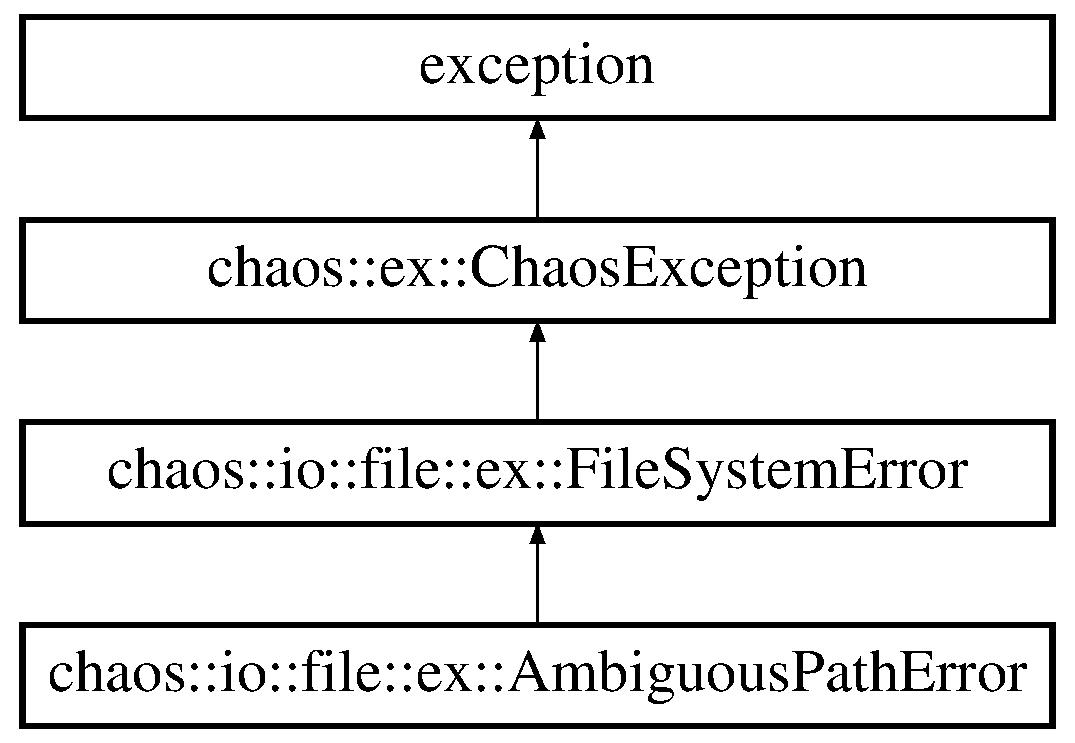
\includegraphics[height=4.000000cm]{classchaos_1_1io_1_1file_1_1ex_1_1_ambiguous_path_error}
\end{center}
\end{figure}
\subsection*{Public Member Functions}
\begin{DoxyCompactItemize}
\item 
\hypertarget{classchaos_1_1io_1_1file_1_1ex_1_1_ambiguous_path_error_a959cd9a1f6204c532cd6f33e29efb84c}{}{\bfseries Ambiguous\+Path\+Error} (const \hyperlink{classchaos_1_1str_1_1_u_t_f8_string}{chaos\+::str\+::\+U\+T\+F8\+String} \&message)\label{classchaos_1_1io_1_1file_1_1ex_1_1_ambiguous_path_error_a959cd9a1f6204c532cd6f33e29efb84c}

\end{DoxyCompactItemize}
\subsection*{Additional Inherited Members}


\subsection{Detailed Description}
Warns that has a request has been made to create a file or directory that results in a ambiguous file system path. 

An example is if a directory called \textquotesingle{}my\+\_\+name\textquotesingle{} was attempted to be created where a file also called \textquotesingle{}my\+\_\+name\textquotesingle{} exists in the same directory. 

The documentation for this class was generated from the following file\+:\begin{DoxyCompactItemize}
\item 
D\+:/\+Dropbox/\+Development/\+Chaos\+Core/\+Chaos\+Core/src/cxx/chaoscore/io/file/\hyperlink{_file_exceptions_8hpp}{File\+Exceptions.\+hpp}\end{DoxyCompactItemize}

\hypertarget{classchaos_1_1ex_1_1_chaos_exception}{}\section{chaos\+:\+:ex\+:\+:Chaos\+Exception Class Reference}
\label{classchaos_1_1ex_1_1_chaos_exception}\index{chaos\+::ex\+::\+Chaos\+Exception@{chaos\+::ex\+::\+Chaos\+Exception}}


Abstract base class that all Chaos\+Core Exceptions extend from.  




{\ttfamily \#include $<$Base\+Exceptions.\+hpp$>$}

Inheritance diagram for chaos\+:\+:ex\+:\+:Chaos\+Exception\+:\begin{figure}[H]
\begin{center}
\leavevmode
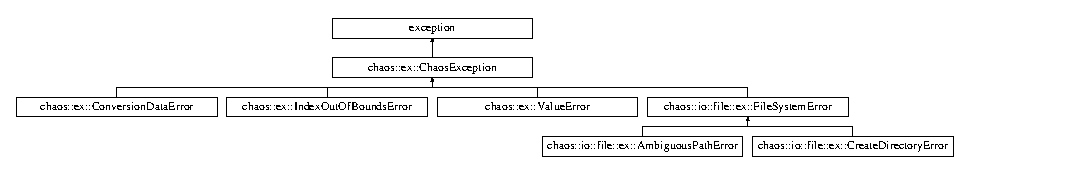
\includegraphics[height=1.171548cm]{classchaos_1_1ex_1_1_chaos_exception}
\end{center}
\end{figure}
\subsection*{Public Member Functions}
\begin{DoxyCompactItemize}
\item 
virtual const char $\ast$ \hyperlink{classchaos_1_1ex_1_1_chaos_exception_a5266c5ba1e7b6ab2bbfcb2a6c01fafea}{what} () const   throw ()
\item 
const \hyperlink{classchaos_1_1uni_1_1_u_t_f8_string}{chaos\+::uni\+::\+U\+T\+F8\+String} \& \hyperlink{classchaos_1_1ex_1_1_chaos_exception_a03cf7cf992d411770c7cefa925c84f4f}{get\+\_\+message} () const 
\end{DoxyCompactItemize}
\subsection*{Protected Member Functions}
\begin{DoxyCompactItemize}
\item 
\hyperlink{classchaos_1_1ex_1_1_chaos_exception_a66463bad3b8d75073ae73c27717ae70d}{Chaos\+Exception} (const \hyperlink{classchaos_1_1uni_1_1_u_t_f8_string}{chaos\+::uni\+::\+U\+T\+F8\+String} \&message)
\begin{DoxyCompactList}\small\item\em Super constructor for objects derived from \hyperlink{classchaos_1_1ex_1_1_chaos_exception}{Chaos\+Exception}. \end{DoxyCompactList}\end{DoxyCompactItemize}


\subsection{Detailed Description}
Abstract base class that all Chaos\+Core Exceptions extend from. 

This class directly inherits from std\+::exception. 

\subsection{Constructor \& Destructor Documentation}
\hypertarget{classchaos_1_1ex_1_1_chaos_exception_a66463bad3b8d75073ae73c27717ae70d}{}\index{chaos\+::ex\+::\+Chaos\+Exception@{chaos\+::ex\+::\+Chaos\+Exception}!Chaos\+Exception@{Chaos\+Exception}}
\index{Chaos\+Exception@{Chaos\+Exception}!chaos\+::ex\+::\+Chaos\+Exception@{chaos\+::ex\+::\+Chaos\+Exception}}
\subsubsection[{Chaos\+Exception(const chaos\+::uni\+::\+U\+T\+F8\+String \&message)}]{\setlength{\rightskip}{0pt plus 5cm}chaos\+::ex\+::\+Chaos\+Exception\+::\+Chaos\+Exception (
\begin{DoxyParamCaption}
\item[{const {\bf chaos\+::uni\+::\+U\+T\+F8\+String} \&}]{message}
\end{DoxyParamCaption}
)\hspace{0.3cm}{\ttfamily [inline]}, {\ttfamily [protected]}}\label{classchaos_1_1ex_1_1_chaos_exception_a66463bad3b8d75073ae73c27717ae70d}


Super constructor for objects derived from \hyperlink{classchaos_1_1ex_1_1_chaos_exception}{Chaos\+Exception}. 


\begin{DoxyParams}{Parameters}
{\em message} & A message decribing the reason for the exception. \\
\hline
\end{DoxyParams}


\subsection{Member Function Documentation}
\hypertarget{classchaos_1_1ex_1_1_chaos_exception_a5266c5ba1e7b6ab2bbfcb2a6c01fafea}{}\index{chaos\+::ex\+::\+Chaos\+Exception@{chaos\+::ex\+::\+Chaos\+Exception}!what@{what}}
\index{what@{what}!chaos\+::ex\+::\+Chaos\+Exception@{chaos\+::ex\+::\+Chaos\+Exception}}
\subsubsection[{what() const }]{\setlength{\rightskip}{0pt plus 5cm}virtual const char$\ast$ chaos\+::ex\+::\+Chaos\+Exception\+::what (
\begin{DoxyParamCaption}
{}
\end{DoxyParamCaption}
) const throw  ) \hspace{0.3cm}{\ttfamily [inline]}, {\ttfamily [virtual]}}\label{classchaos_1_1ex_1_1_chaos_exception_a5266c5ba1e7b6ab2bbfcb2a6c01fafea}
\begin{DoxyReturn}{Returns}
The reason for the exception. 
\end{DoxyReturn}
\hypertarget{classchaos_1_1ex_1_1_chaos_exception_a03cf7cf992d411770c7cefa925c84f4f}{}\index{chaos\+::ex\+::\+Chaos\+Exception@{chaos\+::ex\+::\+Chaos\+Exception}!get\+\_\+message@{get\+\_\+message}}
\index{get\+\_\+message@{get\+\_\+message}!chaos\+::ex\+::\+Chaos\+Exception@{chaos\+::ex\+::\+Chaos\+Exception}}
\subsubsection[{get\+\_\+message() const }]{\setlength{\rightskip}{0pt plus 5cm}const {\bf chaos\+::uni\+::\+U\+T\+F8\+String}\& chaos\+::ex\+::\+Chaos\+Exception\+::get\+\_\+message (
\begin{DoxyParamCaption}
{}
\end{DoxyParamCaption}
) const\hspace{0.3cm}{\ttfamily [inline]}}\label{classchaos_1_1ex_1_1_chaos_exception_a03cf7cf992d411770c7cefa925c84f4f}
\begin{DoxyReturn}{Returns}
The reason for the exception. 
\end{DoxyReturn}


The documentation for this class was generated from the following file\+:\begin{DoxyCompactItemize}
\item 
D\+:/\+Dropbox/\+Development/\+Chaos\+Core/\+Chaos\+Core/src/cxx/chaoscore/base/\hyperlink{_base_exceptions_8hpp}{Base\+Exceptions.\+hpp}\end{DoxyCompactItemize}

\hypertarget{classchaos_1_1ex_1_1_conversion_data_error}{}\section{chaos\+:\+:ex\+:\+:Conversion\+Data\+Error Class Reference}
\label{classchaos_1_1ex_1_1_conversion_data_error}\index{chaos\+::ex\+::\+Conversion\+Data\+Error@{chaos\+::ex\+::\+Conversion\+Data\+Error}}


Warns that the provided data for a type conversion was bad or invalid.  




{\ttfamily \#include $<$Base\+Exceptions.\+hpp$>$}

Inheritance diagram for chaos\+:\+:ex\+:\+:Conversion\+Data\+Error\+:\begin{figure}[H]
\begin{center}
\leavevmode
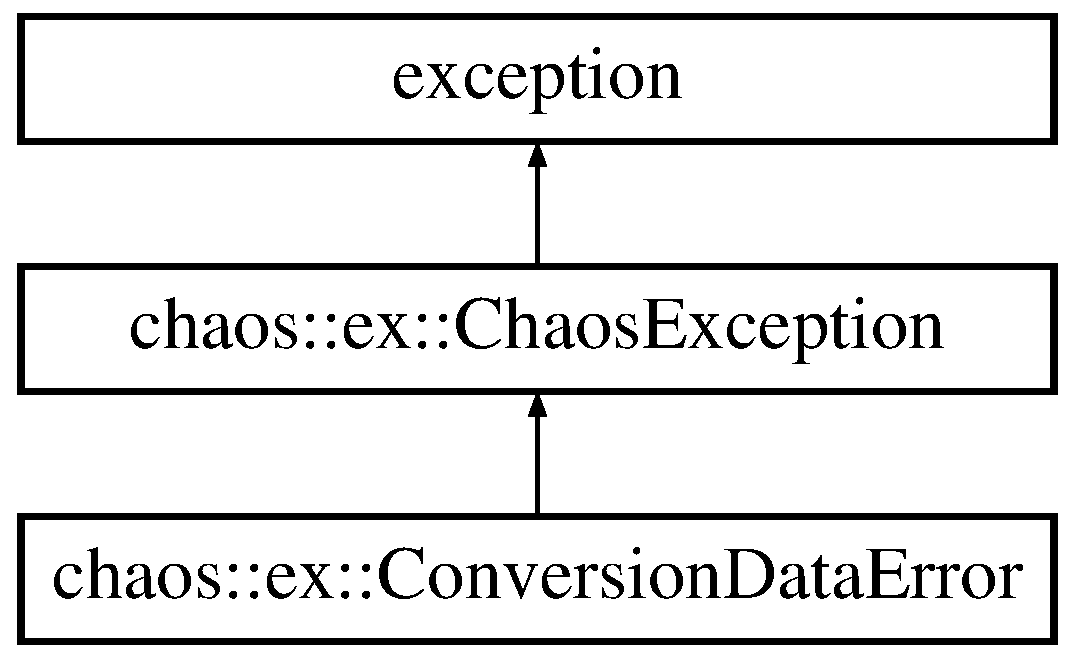
\includegraphics[height=3.000000cm]{classchaos_1_1ex_1_1_conversion_data_error}
\end{center}
\end{figure}
\subsection*{Public Member Functions}
\begin{DoxyCompactItemize}
\item 
\hypertarget{classchaos_1_1ex_1_1_conversion_data_error_afef7fd90707b2bd0be147090613c1222}{}{\bfseries Conversion\+Data\+Error} (const \hyperlink{classchaos_1_1str_1_1_u_t_f8_string}{chaos\+::str\+::\+U\+T\+F8\+String} \&message)\label{classchaos_1_1ex_1_1_conversion_data_error_afef7fd90707b2bd0be147090613c1222}

\end{DoxyCompactItemize}
\subsection*{Additional Inherited Members}


\subsection{Detailed Description}
Warns that the provided data for a type conversion was bad or invalid. 

The documentation for this class was generated from the following file\+:\begin{DoxyCompactItemize}
\item 
D\+:/\+Dropbox/\+Development/\+Chaos\+Core/\+Chaos\+Core/src/cxx/chaoscore/base/\hyperlink{_base_exceptions_8hpp}{Base\+Exceptions.\+hpp}\end{DoxyCompactItemize}

\hypertarget{classchaos_1_1io_1_1file_1_1ex_1_1_create_directory_error}{\section{chaos\-:\-:io\-:\-:file\-:\-:ex\-:\-:Create\-Directory\-Error Class Reference}
\label{classchaos_1_1io_1_1file_1_1ex_1_1_create_directory_error}\index{chaos\-::io\-::file\-::ex\-::\-Create\-Directory\-Error@{chaos\-::io\-::file\-::ex\-::\-Create\-Directory\-Error}}
}


Warns that creating a directory has failed.  




{\ttfamily \#include $<$File\-Exceptions.\-hpp$>$}

Inheritance diagram for chaos\-:\-:io\-:\-:file\-:\-:ex\-:\-:Create\-Directory\-Error\-:\begin{figure}[H]
\begin{center}
\leavevmode
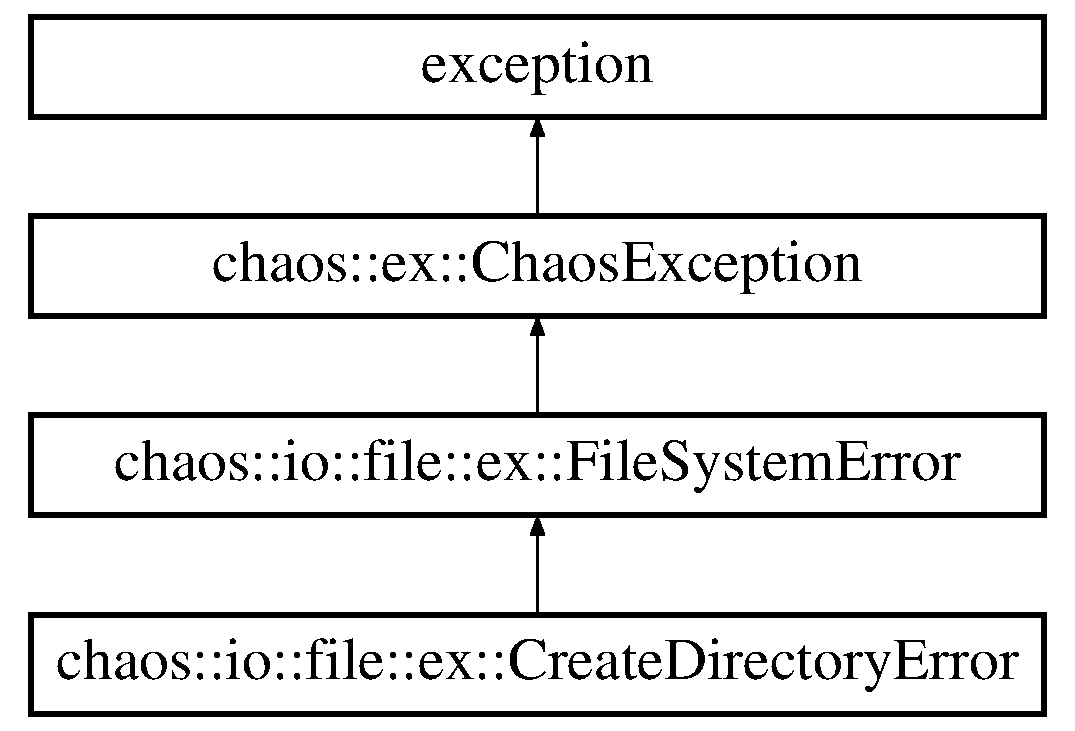
\includegraphics[height=4.000000cm]{classchaos_1_1io_1_1file_1_1ex_1_1_create_directory_error}
\end{center}
\end{figure}
\subsection*{Public Member Functions}
\begin{DoxyCompactItemize}
\item 
\hypertarget{classchaos_1_1io_1_1file_1_1ex_1_1_create_directory_error_a6b468970fd3f8b6f786e0b41becdc019}{{\bfseries Create\-Directory\-Error} (const \hyperlink{classchaos_1_1uni_1_1_u_t_f8_string}{chaos\-::uni\-::\-U\-T\-F8\-String} \&message)}\label{classchaos_1_1io_1_1file_1_1ex_1_1_create_directory_error_a6b468970fd3f8b6f786e0b41becdc019}

\end{DoxyCompactItemize}
\subsection*{Additional Inherited Members}


\subsection{Detailed Description}
Warns that creating a directory has failed. 

The documentation for this class was generated from the following file\-:\begin{DoxyCompactItemize}
\item 
/home/david/\-Dropbox/\-Development/\-Chaos\-Core/\-Chaos\-Core/src/cxx/chaoscore/io/file/\hyperlink{_file_exceptions_8hpp}{File\-Exceptions.\-hpp}\end{DoxyCompactItemize}

\hypertarget{classchaos_1_1io_1_1file_1_1ex_1_1_file_system_error}{}\section{chaos\+:\+:io\+:\+:file\+:\+:ex\+:\+:File\+System\+Error Class Reference}
\label{classchaos_1_1io_1_1file_1_1ex_1_1_file_system_error}\index{chaos\+::io\+::file\+::ex\+::\+File\+System\+Error@{chaos\+::io\+::file\+::ex\+::\+File\+System\+Error}}


A generic error relating to the file system.  




{\ttfamily \#include $<$File\+Exceptions.\+hpp$>$}

Inheritance diagram for chaos\+:\+:io\+:\+:file\+:\+:ex\+:\+:File\+System\+Error\+:\begin{figure}[H]
\begin{center}
\leavevmode
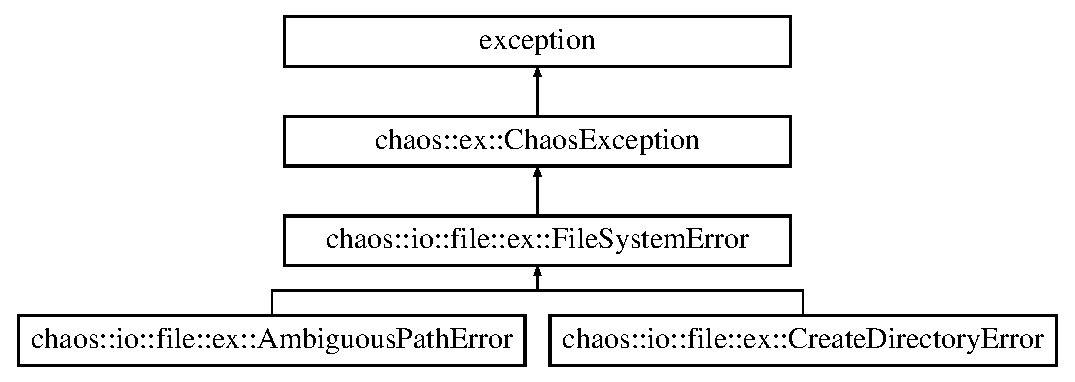
\includegraphics[height=4.000000cm]{classchaos_1_1io_1_1file_1_1ex_1_1_file_system_error}
\end{center}
\end{figure}
\subsection*{Public Member Functions}
\begin{DoxyCompactItemize}
\item 
\hypertarget{classchaos_1_1io_1_1file_1_1ex_1_1_file_system_error_a5164efe6e9bdcd5d9aa222514b6e1b4b}{}{\bfseries File\+System\+Error} (const \hyperlink{classchaos_1_1uni_1_1_u_t_f8_string}{chaos\+::uni\+::\+U\+T\+F8\+String} \&message)\label{classchaos_1_1io_1_1file_1_1ex_1_1_file_system_error_a5164efe6e9bdcd5d9aa222514b6e1b4b}

\end{DoxyCompactItemize}
\subsection*{Additional Inherited Members}


\subsection{Detailed Description}
A generic error relating to the file system. 

All other file system exceptions inherit from this exception. 

The documentation for this class was generated from the following file\+:\begin{DoxyCompactItemize}
\item 
D\+:/\+Dropbox/\+Development/\+Chaos\+Core/\+Chaos\+Core/src/cxx/chaoscore/io/file/\hyperlink{_file_exceptions_8hpp}{File\+Exceptions.\+hpp}\end{DoxyCompactItemize}

\hypertarget{classchaos_1_1test_1_1_fixture}{\section{chaos\-:\-:test\-:\-:Fixture Class Reference}
\label{classchaos_1_1test_1_1_fixture}\index{chaos\-::test\-::\-Fixture@{chaos\-::test\-::\-Fixture}}
}


T\-O\-D\-O\-: D\-O\-C.  




{\ttfamily \#include $<$Chaos\-Test.\-hpp$>$}



\subsection{Detailed Description}
T\-O\-D\-O\-: D\-O\-C. 

T\-O\-D\-O\-: D\-O\-C 

The documentation for this class was generated from the following file\-:\begin{DoxyCompactItemize}
\item 
/home/david/\-Dropbox/\-Development/\-Chaos\-Core/\-Chaos\-Core/src/cxx/chaoscore/test/\hyperlink{_chaos_test_8hpp}{Chaos\-Test.\-hpp}\end{DoxyCompactItemize}

\hypertarget{classchaos_1_1ex_1_1_index_out_of_bounds_error}{\section{chaos\-:\-:ex\-:\-:Index\-Out\-Of\-Bounds\-Error Class Reference}
\label{classchaos_1_1ex_1_1_index_out_of_bounds_error}\index{chaos\-::ex\-::\-Index\-Out\-Of\-Bounds\-Error@{chaos\-::ex\-::\-Index\-Out\-Of\-Bounds\-Error}}
}


Warns that an index has been requested outside of the allowed bounds.  




{\ttfamily \#include $<$Base\-Exceptions.\-hpp$>$}

Inheritance diagram for chaos\-:\-:ex\-:\-:Index\-Out\-Of\-Bounds\-Error\-:\begin{figure}[H]
\begin{center}
\leavevmode
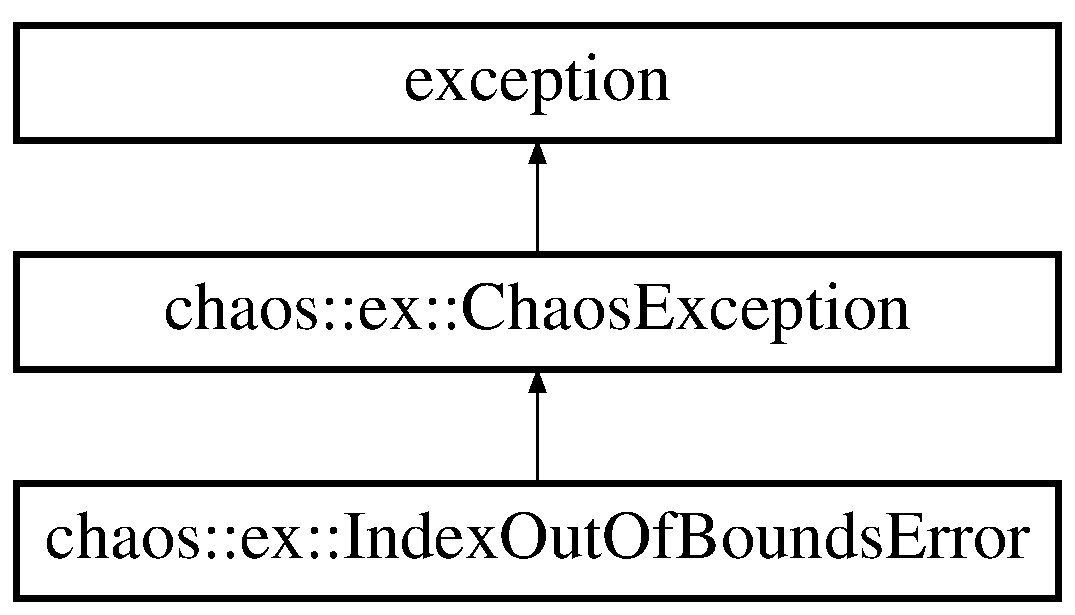
\includegraphics[height=3.000000cm]{classchaos_1_1ex_1_1_index_out_of_bounds_error}
\end{center}
\end{figure}
\subsection*{Public Member Functions}
\begin{DoxyCompactItemize}
\item 
\hypertarget{classchaos_1_1ex_1_1_index_out_of_bounds_error_a605674cdcd80159feffdc66bf4ae36f5}{{\bfseries Index\-Out\-Of\-Bounds\-Error} (const \hyperlink{classchaos_1_1str_1_1_u_t_f8_string}{chaos\-::str\-::\-U\-T\-F8\-String} \&message)}\label{classchaos_1_1ex_1_1_index_out_of_bounds_error_a605674cdcd80159feffdc66bf4ae36f5}

\end{DoxyCompactItemize}
\subsection*{Additional Inherited Members}


\subsection{Detailed Description}
Warns that an index has been requested outside of the allowed bounds. 

The documentation for this class was generated from the following file\-:\begin{DoxyCompactItemize}
\item 
/home/david/\-Dropbox/\-Development/\-Chaos\-Core/\-Chaos\-Core/src/cxx/chaoscore/base/\hyperlink{_base_exceptions_8hpp}{Base\-Exceptions.\-hpp}\end{DoxyCompactItemize}

\hypertarget{classchaos_1_1str_1_1_u_t_f8_string}{\section{chaos\-:\-:str\-:\-:U\-T\-F8\-String Class Reference}
\label{classchaos_1_1str_1_1_u_t_f8_string}\index{chaos\-::str\-::\-U\-T\-F8\-String@{chaos\-::str\-::\-U\-T\-F8\-String}}
}


A string type designed for storing and manipulating U\-T\-F-\/8 encoded text.  




{\ttfamily \#include $<$U\-T\-F8\-String.\-hpp$>$}

\subsection*{Public Member Functions}
\begin{DoxyCompactItemize}
\item 
\hyperlink{classchaos_1_1str_1_1_u_t_f8_string_a173513bf2d62d742bee337b00716bf82}{U\-T\-F8\-String} ()
\begin{DoxyCompactList}\small\item\em Default constructor. \end{DoxyCompactList}\item 
\hyperlink{classchaos_1_1str_1_1_u_t_f8_string_af506696bfe777057c4a7e6b6acf19dab}{U\-T\-F8\-String} (const char $\ast$data)
\begin{DoxyCompactList}\small\item\em C style string constructor. \end{DoxyCompactList}\item 
\hyperlink{classchaos_1_1str_1_1_u_t_f8_string_ac3077c0963a5f36dcaa2a87a1c02d05d}{U\-T\-F8\-String} (const char $\ast$data, size\-\_\-t length)
\begin{DoxyCompactList}\small\item\em C style string and length constructor. \end{DoxyCompactList}\item 
\hyperlink{classchaos_1_1str_1_1_u_t_f8_string_a194b76859245fdb815ce5d537f2e1db4}{U\-T\-F8\-String} (const \hyperlink{classchaos_1_1str_1_1_u_t_f8_string}{U\-T\-F8\-String} \&other)
\begin{DoxyCompactList}\small\item\em Copy constructor. \end{DoxyCompactList}\item 
const \hyperlink{classchaos_1_1str_1_1_u_t_f8_string}{U\-T\-F8\-String} \& \hyperlink{classchaos_1_1str_1_1_u_t_f8_string_a050b804cc8978a4a55a5bc0a8cad2553}{operator=} (const \hyperlink{classchaos_1_1str_1_1_u_t_f8_string}{U\-T\-F8\-String} \&other)
\begin{DoxyCompactList}\small\item\em Assignment operator. \end{DoxyCompactList}\item 
bool \hyperlink{classchaos_1_1str_1_1_u_t_f8_string_ae4446150398d498e8aa9ebbc05ca7b52}{operator==} (const \hyperlink{classchaos_1_1str_1_1_u_t_f8_string}{U\-T\-F8\-String} \&other) const 
\begin{DoxyCompactList}\small\item\em Equality operator. \end{DoxyCompactList}\item 
bool \hyperlink{classchaos_1_1str_1_1_u_t_f8_string_a166394399a4d200494b40e034aa330da}{operator!=} (const \hyperlink{classchaos_1_1str_1_1_u_t_f8_string}{U\-T\-F8\-String} \&other) const 
\begin{DoxyCompactList}\small\item\em Inequality operator. \end{DoxyCompactList}\item 
bool \hyperlink{classchaos_1_1str_1_1_u_t_f8_string_ac7b54ed9c42a9c9a0a386d453d2c1daa}{operator$<$} (const \hyperlink{classchaos_1_1str_1_1_u_t_f8_string}{U\-T\-F8\-String} \&other) const 
\begin{DoxyCompactList}\small\item\em Less than operator. \end{DoxyCompactList}\item 
\hyperlink{classchaos_1_1str_1_1_u_t_f8_string}{U\-T\-F8\-String} \hyperlink{classchaos_1_1str_1_1_u_t_f8_string_a0d624a8e308b9a04511d31558ae37d8d}{operator+} (const \hyperlink{classchaos_1_1str_1_1_u_t_f8_string}{U\-T\-F8\-String} \&other) const 
\begin{DoxyCompactList}\small\item\em Addition operator. \end{DoxyCompactList}\item 
const \hyperlink{classchaos_1_1str_1_1_u_t_f8_string}{U\-T\-F8\-String} \& \hyperlink{classchaos_1_1str_1_1_u_t_f8_string_a9ce7f005abc581590ff3823db749873f}{operator+=} (const \hyperlink{classchaos_1_1str_1_1_u_t_f8_string}{U\-T\-F8\-String} \&other)
\begin{DoxyCompactList}\small\item\em Compound addition operator. \end{DoxyCompactList}\item 
\hyperlink{classchaos_1_1str_1_1_u_t_f8_string}{U\-T\-F8\-String} \hyperlink{classchaos_1_1str_1_1_u_t_f8_string_a782fc0fcf19f6b9646ca962f2bd8a214}{operator$\ast$} (\hyperlink{namespacechaos_a3b3a47ba1e284655bf1a30c441121c60}{chaos\-::uint32} count) const 
\begin{DoxyCompactList}\small\item\em Multiplication operator. \end{DoxyCompactList}\item 
const \hyperlink{classchaos_1_1str_1_1_u_t_f8_string}{U\-T\-F8\-String} \& \hyperlink{classchaos_1_1str_1_1_u_t_f8_string_a653dcbb095d2db19042807d03372dfbd}{operator$\ast$=} (\hyperlink{namespacechaos_a3b3a47ba1e284655bf1a30c441121c60}{chaos\-::uint32} count)
\begin{DoxyCompactList}\small\item\em Compound multiplication operator. \end{DoxyCompactList}\item 
\hyperlink{classchaos_1_1str_1_1_u_t_f8_string}{U\-T\-F8\-String} \& \hyperlink{classchaos_1_1str_1_1_u_t_f8_string_a3ab14e1ddffbadd664ebd4f228d11f17}{operator$<$$<$} (const \hyperlink{classchaos_1_1str_1_1_u_t_f8_string}{U\-T\-F8\-String} \&other)
\begin{DoxyCompactList}\small\item\em Stream operator. \end{DoxyCompactList}\item 
\hyperlink{classchaos_1_1str_1_1_u_t_f8_string}{U\-T\-F8\-String} \& \hyperlink{classchaos_1_1str_1_1_u_t_f8_string_ac3ca865b7f68b13b4b5902793bbb750d}{operator$<$$<$} (const char $\ast$other)
\begin{DoxyCompactList}\small\item\em Stream operator. \end{DoxyCompactList}\item 
\hyperlink{classchaos_1_1str_1_1_u_t_f8_string}{U\-T\-F8\-String} \& \hyperlink{classchaos_1_1str_1_1_u_t_f8_string_a083f1107b391e5b4854ff40bc09c1406}{operator$<$$<$} (const std\-::string \&other)
\begin{DoxyCompactList}\small\item\em Stream operator. \end{DoxyCompactList}\item 
\hyperlink{classchaos_1_1str_1_1_u_t_f8_string}{U\-T\-F8\-String} \& \hyperlink{classchaos_1_1str_1_1_u_t_f8_string_a9ef346ef5d7211de67578ce4bcc4a122}{operator$<$$<$} (bool other)
\begin{DoxyCompactList}\small\item\em Stream operator. \end{DoxyCompactList}\item 
\hyperlink{classchaos_1_1str_1_1_u_t_f8_string}{U\-T\-F8\-String} \& \hyperlink{classchaos_1_1str_1_1_u_t_f8_string_a1fe072a86408b3eb0b3fdfe9f80e3b8d}{operator$<$$<$} (char other)
\begin{DoxyCompactList}\small\item\em Stream operator. \end{DoxyCompactList}\item 
\hyperlink{classchaos_1_1str_1_1_u_t_f8_string}{U\-T\-F8\-String} \& \hyperlink{classchaos_1_1str_1_1_u_t_f8_string_a89937311871b473ed17bd83622e60530}{operator$<$$<$} (\hyperlink{namespacechaos_a56015674cfe4ad1fc583c3da6c724d8a}{chaos\-::int8} other)
\begin{DoxyCompactList}\small\item\em Stream operator. \end{DoxyCompactList}\item 
\hyperlink{classchaos_1_1str_1_1_u_t_f8_string}{U\-T\-F8\-String} \& \hyperlink{classchaos_1_1str_1_1_u_t_f8_string_abfce18f938382812ffeb3c399fdf679e}{operator$<$$<$} (\hyperlink{namespacechaos_a229e18634387996c2712d57f184bf363}{chaos\-::uint8} other)
\begin{DoxyCompactList}\small\item\em Stream operator. \end{DoxyCompactList}\item 
\hyperlink{classchaos_1_1str_1_1_u_t_f8_string}{U\-T\-F8\-String} \& \hyperlink{classchaos_1_1str_1_1_u_t_f8_string_a970df73b6bbb3d31fe5bcf53bc654be6}{operator$<$$<$} (\hyperlink{namespacechaos_a23112b8188c8a6ad32a86041fb4c088e}{chaos\-::int16} other)
\begin{DoxyCompactList}\small\item\em Stream operator. \end{DoxyCompactList}\item 
\hyperlink{classchaos_1_1str_1_1_u_t_f8_string}{U\-T\-F8\-String} \& \hyperlink{classchaos_1_1str_1_1_u_t_f8_string_aa1ae66a5b283279df734eab632e398cf}{operator$<$$<$} (\hyperlink{namespacechaos_ac3888b1c9e56da7fbbdb3ab8425b4068}{chaos\-::uint16} other)
\begin{DoxyCompactList}\small\item\em Stream operator. \end{DoxyCompactList}\item 
\hyperlink{classchaos_1_1str_1_1_u_t_f8_string}{U\-T\-F8\-String} \& \hyperlink{classchaos_1_1str_1_1_u_t_f8_string_a1c174fd024e1535a2f485e290540a2a1}{operator$<$$<$} (\hyperlink{namespacechaos_ad1de7efb430365afd2c9446a0f522a90}{chaos\-::int32} other)
\begin{DoxyCompactList}\small\item\em Stream operator. \end{DoxyCompactList}\item 
\hyperlink{classchaos_1_1str_1_1_u_t_f8_string}{U\-T\-F8\-String} \& \hyperlink{classchaos_1_1str_1_1_u_t_f8_string_a99aa07fcc88a65befe5e530933839fab}{operator$<$$<$} (\hyperlink{namespacechaos_a3b3a47ba1e284655bf1a30c441121c60}{chaos\-::uint32} other)
\begin{DoxyCompactList}\small\item\em Stream operator. \end{DoxyCompactList}\item 
\hyperlink{classchaos_1_1str_1_1_u_t_f8_string}{U\-T\-F8\-String} \& \hyperlink{classchaos_1_1str_1_1_u_t_f8_string_a5fac3cdc0e1aa0bdefce09a0dab085cf}{operator$<$$<$} (\hyperlink{namespacechaos_a46c61f58d99879b936f58234b9a05e0c}{chaos\-::int64} other)
\begin{DoxyCompactList}\small\item\em Stream operator. \end{DoxyCompactList}\item 
\hyperlink{classchaos_1_1str_1_1_u_t_f8_string}{U\-T\-F8\-String} \& \hyperlink{classchaos_1_1str_1_1_u_t_f8_string_a0f069c833c4fad2e87f9e4fb1138eca6}{operator$<$$<$} (\hyperlink{namespacechaos_a34fe5f5bfc3ef6d80b5d094ed91b4d6e}{chaos\-::uint64} other)
\begin{DoxyCompactList}\small\item\em Stream operator. \end{DoxyCompactList}\item 
void \hyperlink{classchaos_1_1str_1_1_u_t_f8_string_a483e71ec1090e346c63bf2b13b37ad7a}{assign} (const char $\ast$data)
\begin{DoxyCompactList}\small\item\em Assigns the internal data of this \hyperlink{classchaos_1_1str_1_1_u_t_f8_string}{U\-T\-F8\-String} from the given C style string. \end{DoxyCompactList}\item 
void \hyperlink{classchaos_1_1str_1_1_u_t_f8_string_a631f935a5b85214a2fa662a78f5693aa}{assign} (const char $\ast$data, size\-\_\-t length)
\begin{DoxyCompactList}\small\item\em Assigns the internal data of this \hyperlink{classchaos_1_1str_1_1_u_t_f8_string}{U\-T\-F8\-String} from the given C style string and byte length. \end{DoxyCompactList}\item 
void \hyperlink{classchaos_1_1str_1_1_u_t_f8_string_aff351b1a6276e5e59717bc6c3b67818c}{assign} (const \hyperlink{classchaos_1_1str_1_1_u_t_f8_string}{U\-T\-F8\-String} \&other)
\begin{DoxyCompactList}\small\item\em Assigns internal data from a copy of another \hyperlink{classchaos_1_1str_1_1_u_t_f8_string}{U\-T\-F8\-String}. \end{DoxyCompactList}\item 
\hyperlink{classchaos_1_1str_1_1_u_t_f8_string}{U\-T\-F8\-String} \& \hyperlink{classchaos_1_1str_1_1_u_t_f8_string_a8b61a2f73dacd4749d993dad00788d0d}{concatenate} (const \hyperlink{classchaos_1_1str_1_1_u_t_f8_string}{U\-T\-F8\-String} \&other)
\begin{DoxyCompactList}\small\item\em Concatenates another \hyperlink{classchaos_1_1str_1_1_u_t_f8_string}{U\-T\-F8\-String} on to the end of this string. \end{DoxyCompactList}\item 
\hyperlink{classchaos_1_1str_1_1_u_t_f8_string}{U\-T\-F8\-String} \& \hyperlink{classchaos_1_1str_1_1_u_t_f8_string_a5a497616981f69154c1c4924a486c41d}{repeat} (\hyperlink{namespacechaos_a3b3a47ba1e284655bf1a30c441121c60}{chaos\-::uint32} count)
\begin{DoxyCompactList}\small\item\em Extends this string with a copy of itself the given number of times. \end{DoxyCompactList}\item 
bool \hyperlink{classchaos_1_1str_1_1_u_t_f8_string_a065a34c88630d3aca883d691322474c0}{starts\-\_\-with} (const \hyperlink{classchaos_1_1str_1_1_u_t_f8_string}{U\-T\-F8\-String} \&\hyperlink{classchaos_1_1str_1_1_u_t_f8_string_a2d50ab58715264ae175f521816bf670c}{substring}) const 
\begin{DoxyCompactList}\small\item\em Checks whether this \hyperlink{classchaos_1_1str_1_1_u_t_f8_string}{U\-T\-F8\-String} starts with the given substring. \end{DoxyCompactList}\item 
size\-\_\-t \hyperlink{classchaos_1_1str_1_1_u_t_f8_string_a035c9c2a40bcac212ebb20a8524d0b5a}{find\-\_\-first} (const \hyperlink{classchaos_1_1str_1_1_u_t_f8_string}{U\-T\-F8\-String} \&\hyperlink{classchaos_1_1str_1_1_u_t_f8_string_a2d50ab58715264ae175f521816bf670c}{substring}) const 
\begin{DoxyCompactList}\small\item\em Finds the first occurrence of the given substring and returns the symbol index of it within this \hyperlink{classchaos_1_1str_1_1_u_t_f8_string}{U\-T\-F8\-String}. \end{DoxyCompactList}\item 
size\-\_\-t \hyperlink{classchaos_1_1str_1_1_u_t_f8_string_a4053c128303a753735295b441e439933}{find\-\_\-last} (const \hyperlink{classchaos_1_1str_1_1_u_t_f8_string}{U\-T\-F8\-String} \&\hyperlink{classchaos_1_1str_1_1_u_t_f8_string_a2d50ab58715264ae175f521816bf670c}{substring}) const 
\begin{DoxyCompactList}\small\item\em Finds the last occurrence of the given substring and returns the index of it within this \hyperlink{classchaos_1_1str_1_1_u_t_f8_string}{U\-T\-F8\-String}. \end{DoxyCompactList}\item 
const std\-::vector$<$ \hyperlink{classchaos_1_1str_1_1_u_t_f8_string}{U\-T\-F8\-String} $>$ \hyperlink{classchaos_1_1str_1_1_u_t_f8_string_ac5da4c989f6394c38b0fb82a252099db}{split} (const \hyperlink{classchaos_1_1str_1_1_u_t_f8_string}{U\-T\-F8\-String} \&delimiter) const 
\begin{DoxyCompactList}\small\item\em Splits this \hyperlink{classchaos_1_1str_1_1_u_t_f8_string}{U\-T\-F8\-String} by the given delimiter and returns the split elements in a std\-::vector. \end{DoxyCompactList}\item 
bool \hyperlink{classchaos_1_1str_1_1_u_t_f8_string_a64f529f30034281560805b97826c5e13}{is\-\_\-int} () const 
\begin{DoxyCompactList}\small\item\em Whether the symbols of this string make up a valid integer type. \end{DoxyCompactList}\item 
bool \hyperlink{classchaos_1_1str_1_1_u_t_f8_string_a989763da3e7eed8664cd2e5c41ea7e00}{is\-\_\-uint} () const 
\begin{DoxyCompactList}\small\item\em Whether the symbols of this string make up a valid unsigned integer type. \end{DoxyCompactList}\item 
bool \hyperlink{classchaos_1_1str_1_1_u_t_f8_string_a2fbd69fb90a390df37c119577d4d3c6a}{is\-\_\-float} () const 
\begin{DoxyCompactList}\small\item\em Whether the symbols of this string make up a valid floating point type. \end{DoxyCompactList}\item 
\hyperlink{classchaos_1_1str_1_1_u_t_f8_string}{U\-T\-F8\-String} \hyperlink{classchaos_1_1str_1_1_u_t_f8_string_a2d50ab58715264ae175f521816bf670c}{substring} (size\-\_\-t start, size\-\_\-t length) const 
\begin{DoxyCompactList}\small\item\em Returns a new \hyperlink{classchaos_1_1str_1_1_u_t_f8_string}{U\-T\-F8\-String} composed of a substring of this string. \end{DoxyCompactList}\item 
const char $\ast$ \hyperlink{classchaos_1_1str_1_1_u_t_f8_string_aa6fd66af34d7a3c4a495860952e97557}{to\-\_\-cstring} () const 
\begin{DoxyCompactList}\small\item\em Gets the raw byte data of this \hyperlink{classchaos_1_1str_1_1_u_t_f8_string}{U\-T\-F8\-String} as C style string ({\ttfamily const char$\ast$}). \end{DoxyCompactList}\item 
std\-::string \hyperlink{classchaos_1_1str_1_1_u_t_f8_string_a8901fbbe5e72d7bf8f0d160b55475244}{to\-\_\-std\-\_\-string} () const 
\begin{DoxyCompactList}\small\item\em Returns this as a standard library string. \end{DoxyCompactList}\item 
bool \hyperlink{classchaos_1_1str_1_1_u_t_f8_string_abea65bae8fc882d3bacb91aa2befe0b1}{to\-\_\-bool} () const 
\begin{DoxyCompactList}\small\item\em Returns this \hyperlink{classchaos_1_1str_1_1_u_t_f8_string}{U\-T\-F8\-String} as an bool type. \end{DoxyCompactList}\item 
\hyperlink{namespacechaos_ad1de7efb430365afd2c9446a0f522a90}{chaos\-::int32} \hyperlink{classchaos_1_1str_1_1_u_t_f8_string_a17309b0f4d25be1b83a188883c4a9861}{to\-\_\-int32} () const 
\begin{DoxyCompactList}\small\item\em Returns this \hyperlink{classchaos_1_1str_1_1_u_t_f8_string}{U\-T\-F8\-String} as an int32 type. \end{DoxyCompactList}\item 
\hyperlink{namespacechaos_a3b3a47ba1e284655bf1a30c441121c60}{chaos\-::uint32} \hyperlink{classchaos_1_1str_1_1_u_t_f8_string_a85ec2ebfdb419a3422cf87497cabdd86}{to\-\_\-uint32} () const 
\begin{DoxyCompactList}\small\item\em Returns this \hyperlink{classchaos_1_1str_1_1_u_t_f8_string}{U\-T\-F8\-String} as an uint32 type. \end{DoxyCompactList}\item 
\hyperlink{namespacechaos_a46c61f58d99879b936f58234b9a05e0c}{chaos\-::int64} \hyperlink{classchaos_1_1str_1_1_u_t_f8_string_a18eee1b350d45995e43ef41cfd8bb92a}{to\-\_\-int64} () const 
\begin{DoxyCompactList}\small\item\em Returns this \hyperlink{classchaos_1_1str_1_1_u_t_f8_string}{U\-T\-F8\-String} as an int64 type. \end{DoxyCompactList}\item 
\hyperlink{namespacechaos_a46c61f58d99879b936f58234b9a05e0c}{chaos\-::int64} \hyperlink{classchaos_1_1str_1_1_u_t_f8_string_a5ef3a02131444e2a90b634dad7edb19e}{to\-\_\-uint64} () const 
\begin{DoxyCompactList}\small\item\em Returns this \hyperlink{classchaos_1_1str_1_1_u_t_f8_string}{U\-T\-F8\-String} as an uint64 type. \end{DoxyCompactList}\item 
size\-\_\-t \hyperlink{classchaos_1_1str_1_1_u_t_f8_string_ac0c724e649182e02462b48b94d1f5bf7}{get\-\_\-length} () const 
\begin{DoxyCompactList}\small\item\em Returns the number of symbols in this \hyperlink{classchaos_1_1str_1_1_u_t_f8_string}{U\-T\-F8\-String}. \end{DoxyCompactList}\item 
bool \hyperlink{classchaos_1_1str_1_1_u_t_f8_string_a4fc296e90fbbc45a1e3f142dcd1e9853}{is\-\_\-empty} () const 
\begin{DoxyCompactList}\small\item\em Returns whether the this \hyperlink{classchaos_1_1str_1_1_u_t_f8_string}{U\-T\-F8\-String} contains any characters or not. \end{DoxyCompactList}\item 
\hyperlink{classchaos_1_1str_1_1_u_t_f8_string}{U\-T\-F8\-String} \hyperlink{classchaos_1_1str_1_1_u_t_f8_string_a04dbe9f15dc1b09c858e2450de26d40a}{get\-\_\-symbol} (size\-\_\-t index) const 
\begin{DoxyCompactList}\small\item\em Returns the U\-T\-F-\/8 symbol at the given index in this string. \end{DoxyCompactList}\item 
\hyperlink{namespacechaos_a3b3a47ba1e284655bf1a30c441121c60}{chaos\-::uint32} \hyperlink{classchaos_1_1str_1_1_u_t_f8_string_a1248ee0dde0ff8e028d162cefd67f034}{get\-\_\-symbol\-\_\-value} (size\-\_\-t index) const 
\begin{DoxyCompactList}\small\item\em Returns the integer/hex value for the U\-T\-F-\/8 symbol at the given index in this string. \end{DoxyCompactList}\item 
\hyperlink{namespacechaos_a3b3a47ba1e284655bf1a30c441121c60}{chaos\-::uint32} \hyperlink{classchaos_1_1str_1_1_u_t_f8_string_a007889a60f57ec9196dcebb39abeafdf}{get\-\_\-code\-\_\-point} (size\-\_\-t index) const 
\begin{DoxyCompactList}\small\item\em Returns the Unicode code point for the U\-T\-F-\/8 symbol at the given index in this string. \end{DoxyCompactList}\item 
size\-\_\-t \hyperlink{classchaos_1_1str_1_1_u_t_f8_string_a4dddd9c6133754f5f424033ab28dc0e5}{get\-\_\-byte\-\_\-index\-\_\-for\-\_\-symbol\-\_\-index} (size\-\_\-t symbol\-\_\-index) const 
\begin{DoxyCompactList}\small\item\em Gets the index of the first byte for the symbol at the given index in this string. \end{DoxyCompactList}\item 
size\-\_\-t \hyperlink{classchaos_1_1str_1_1_u_t_f8_string_a0c54a7cfaf4a3c1881b0c933c49a4922}{get\-\_\-symbol\-\_\-width} (size\-\_\-t index) const 
\begin{DoxyCompactList}\small\item\em Gets the number of bytes in the symbol at the given index in this string. \end{DoxyCompactList}\item 
size\-\_\-t \hyperlink{classchaos_1_1str_1_1_u_t_f8_string_a9312a6aac333d68a87066d6f222d119a}{get\-\_\-byte\-\_\-length} () const 
\begin{DoxyCompactList}\small\item\em Returns the length of the internal data in bytes. \end{DoxyCompactList}\item 
size\-\_\-t \hyperlink{classchaos_1_1str_1_1_u_t_f8_string_aa005c8b0243343ec7308d00fa6e72846}{get\-\_\-symbol\-\_\-index\-\_\-for\-\_\-byte\-\_\-index} (size\-\_\-t byte\-\_\-index) const 
\begin{DoxyCompactList}\small\item\em Returns the index of the symbol that the byte at the given index is part of. \end{DoxyCompactList}\item 
size\-\_\-t \hyperlink{classchaos_1_1str_1_1_u_t_f8_string_a387abdce2189a379961844cd0a42a97a}{get\-\_\-byte\-\_\-width} (size\-\_\-t byte\-\_\-index) const 
\begin{DoxyCompactList}\small\item\em Returns the number of bytes in the symbol at the given byte index. \end{DoxyCompactList}\end{DoxyCompactItemize}
\subsection*{Static Public Attributes}
\begin{DoxyCompactItemize}
\item 
\hypertarget{classchaos_1_1str_1_1_u_t_f8_string_a7e301ebfad4cd1b14e3a13cb0595b43b}{static const size\-\_\-t \hyperlink{classchaos_1_1str_1_1_u_t_f8_string_a7e301ebfad4cd1b14e3a13cb0595b43b}{npos}}\label{classchaos_1_1str_1_1_u_t_f8_string_a7e301ebfad4cd1b14e3a13cb0595b43b}

\begin{DoxyCompactList}\small\item\em Value that is used to return an index that does not exists within the \hyperlink{classchaos_1_1str_1_1_u_t_f8_string}{U\-T\-F8\-String}. \end{DoxyCompactList}\end{DoxyCompactItemize}


\subsection{Detailed Description}
A string type designed for storing and manipulating U\-T\-F-\/8 encoded text. 

\begin{DoxyNote}{Note}
This object expects input text to already be U\-T\-F-\/8 encoded. For functions to convert encodings see \hyperlink{_unicode_operations_8hpp}{Unicode\-Operations.\-hpp}
\end{DoxyNote}
The \hyperlink{classchaos_1_1str_1_1_u_t_f8_string}{U\-T\-F8\-String} data type is used extensively throughout Chaos\-Core and other Chaos Foundation projects.

Chaos\-Core stands by the principle that all string handling should be Unicode aware. The {\ttfamily char} primitive should only be used for storing and manipulation raw byte data, not for representing entire language characters. Furthermore Chaos\-Core considers U\-T\-F-\/8 to be the only default encoding type for Unicode text. Other encodings should only be used for special cases or interacting with applications that require a different encoding (such as the Windows A\-P\-I). For more info see \href{http://utf8everywhere.org/}{\tt http\-://utf8everywhere.\-org/}

For practicality the internal byte of an \hyperlink{classchaos_1_1str_1_1_u_t_f8_string}{U\-T\-F8\-String} is N\-U\-L\-L terminated. This means the raw data can easily be used as native C style strings.

\begin{DoxyParagraph}{A Brief Introduction to U\-T\-F-\/8}

\end{DoxyParagraph}
In order to fully make use of the \hyperlink{classchaos_1_1str_1_1_u_t_f8_string}{U\-T\-F8\-String} type's functionality its useful to understand the U\-T\-F-\/8 encoding method.

U\-T\-F-\/8 encodes each Unicode symbol in 1-\/4 bytes. The value of each symbol maps directly to a Unicode code point that represents the symbol. For example\-:


\begin{DoxyItemize}
\item \char`\"{}a\char`\"{} is stored using one byte with the hex value 0x61 or binary value {\ttfamily 01100001}
\item \char`\"{}ל\char`\"{} is stored using two bytes with the hex value 0x\-D79\-C or binary value {\ttfamily 11010111 10011100}
\item \char`\"{}∑\char`\"{} is stored using three bytes with the hex value 0x\-E28891 or binary value {\ttfamily 11100010 10001000 10010001}
\item \char`\"{}𝄞\char`\"{} is stored using four bytes with the hex value 0x\-F09\-D849\-E or binary value {\ttfamily 11110000 10011101 10000100 10011110}
\end{DoxyItemize}

The byte size of a U\-T\-F-\/8 symbol can be recognised by the bit pattern that makes up the start of each byte\-:


\begin{DoxyItemize}
\item One byte symbol\-: {\ttfamily 0xxxxxxx}
\item Two byte symbol\-: {\ttfamily 110xxxxx 10xxxxxx}
\item Three byte symbol\-: {\ttfamily 1110xxxx 10xxxxxx 10xxxxxx}
\item Four byte symbol\-: {\ttfamily 11110xxx 10xxxxxx 10xxxxxx 10xxxxxx}
\end{DoxyItemize}

\begin{DoxyParagraph}{U\-T\-F8\-String Usage}

\end{DoxyParagraph}
Here follows an example of using the \hyperlink{classchaos_1_1str_1_1_u_t_f8_string}{U\-T\-F8\-String} type\-:

We have a C style string that cannot be encoded correctly with A\-S\-C\-I\-I (In this case we are assuming the input string is encoded in U\-T\-F-\/8)\-:


\begin{DoxyCode}
\textcolor{keyword}{const} \textcolor{keywordtype}{char}* cstring = \textcolor{stringliteral}{"aל∑"};
\end{DoxyCode}


If we inspect the length of the string we get unexpected results\-:


\begin{DoxyCode}
strlen( cstring );
\textcolor{comment}{// output: 6}
\end{DoxyCode}


This is because while the string only contains 3 symbols it contains 6 bytes which is what {\ttfamily strlen} is counting. Next we construct a \hyperlink{classchaos_1_1str_1_1_u_t_f8_string}{U\-T\-F8\-String} using the c string data, and inspect it's length\-:


\begin{DoxyCode}
\hyperlink{classchaos_1_1str_1_1_u_t_f8_string}{chaos::str::UTF8String} utf8( cstring );
utf8.get\_length();
\textcolor{comment}{// output: 3}
utf8.get\_byte\_length()
\textcolor{comment}{// output: 6}
\end{DoxyCode}


\mbox{[}T\-O\-D\-O\-: iterator\mbox{]} We can now inspect each symbol in the string\-:


\begin{DoxyCode}
\textcolor{keywordflow}{for} ( \textcolor{keywordtype}{size\_t} i = 0; i < utf8.get\_length(); ++i )
\{
    \hyperlink{classchaos_1_1str_1_1_u_t_f8_string}{chaos::str::UTF8String} symbol( utf8.get\_symbol( i ) );
\}
\end{DoxyCode}


Note that the symbol is returned as an \hyperlink{classchaos_1_1str_1_1_u_t_f8_string}{U\-T\-F8\-String} itself, this is due to the fact that symbol has a variable byte-\/width so cannot be stored in a {\ttfamily char}, nor is there any need to differentiate data types between a string of symbols and an individual symbol.

We can also inspect the byte-\/widths of each symbol in our string\-:


\begin{DoxyCode}
\textcolor{keywordflow}{for} ( \textcolor{keywordtype}{size\_t} i = 0; i < utf8.get\_length(); ++i )
\{
    utf8.get\_symbol\_width( i );
\}
\textcolor{comment}{// output: 1}
\textcolor{comment}{// output: 2}
\textcolor{comment}{// output: 3}
\end{DoxyCode}


The \hyperlink{classchaos_1_1str_1_1_u_t_f8_string}{U\-T\-F8\-String} class provides many convenience functions for manipulating string data, such as {\ttfamily split}, {\ttfamily trim}, {\ttfamily starts\-\_\-with}, {\ttfamily find\-\_\-first}, {\ttfamily to\-\_\-cstring}, {\ttfamily to\-\_\-stdstring}, etc.  

\subsection{Constructor \& Destructor Documentation}
\hypertarget{classchaos_1_1str_1_1_u_t_f8_string_a173513bf2d62d742bee337b00716bf82}{\index{chaos\-::str\-::\-U\-T\-F8\-String@{chaos\-::str\-::\-U\-T\-F8\-String}!U\-T\-F8\-String@{U\-T\-F8\-String}}
\index{U\-T\-F8\-String@{U\-T\-F8\-String}!chaos::str::UTF8String@{chaos\-::str\-::\-U\-T\-F8\-String}}
\subsubsection[{U\-T\-F8\-String}]{\setlength{\rightskip}{0pt plus 5cm}chaos\-::str\-::\-U\-T\-F8\-String\-::\-U\-T\-F8\-String (
\begin{DoxyParamCaption}
{}
\end{DoxyParamCaption}
)}}\label{classchaos_1_1str_1_1_u_t_f8_string_a173513bf2d62d742bee337b00716bf82}


Default constructor. 

Creates a new \hyperlink{classchaos_1_1str_1_1_u_t_f8_string}{U\-T\-F8\-String} that contains no symbols and holds only the N\-U\-L\-L terminator. \hypertarget{classchaos_1_1str_1_1_u_t_f8_string_af506696bfe777057c4a7e6b6acf19dab}{\index{chaos\-::str\-::\-U\-T\-F8\-String@{chaos\-::str\-::\-U\-T\-F8\-String}!U\-T\-F8\-String@{U\-T\-F8\-String}}
\index{U\-T\-F8\-String@{U\-T\-F8\-String}!chaos::str::UTF8String@{chaos\-::str\-::\-U\-T\-F8\-String}}
\subsubsection[{U\-T\-F8\-String}]{\setlength{\rightskip}{0pt plus 5cm}chaos\-::str\-::\-U\-T\-F8\-String\-::\-U\-T\-F8\-String (
\begin{DoxyParamCaption}
\item[{const char $\ast$}]{data}
\end{DoxyParamCaption}
)}}\label{classchaos_1_1str_1_1_u_t_f8_string_af506696bfe777057c4a7e6b6acf19dab}


C style string constructor. 

Creates a new \hyperlink{classchaos_1_1str_1_1_u_t_f8_string}{U\-T\-F8\-String} that contains the provided data.

\begin{DoxyNote}{Note}
The input data is expected to be U\-T\-F-\/8 encoded and N\-U\-L\-L terminated. For functions to convert encodings see \hyperlink{_unicode_operations_8hpp}{Unicode\-Operations.\-hpp} 
\end{DoxyNote}
\hypertarget{classchaos_1_1str_1_1_u_t_f8_string_ac3077c0963a5f36dcaa2a87a1c02d05d}{\index{chaos\-::str\-::\-U\-T\-F8\-String@{chaos\-::str\-::\-U\-T\-F8\-String}!U\-T\-F8\-String@{U\-T\-F8\-String}}
\index{U\-T\-F8\-String@{U\-T\-F8\-String}!chaos::str::UTF8String@{chaos\-::str\-::\-U\-T\-F8\-String}}
\subsubsection[{U\-T\-F8\-String}]{\setlength{\rightskip}{0pt plus 5cm}chaos\-::str\-::\-U\-T\-F8\-String\-::\-U\-T\-F8\-String (
\begin{DoxyParamCaption}
\item[{const char $\ast$}]{data, }
\item[{size\-\_\-t}]{length}
\end{DoxyParamCaption}
)}}\label{classchaos_1_1str_1_1_u_t_f8_string_ac3077c0963a5f36dcaa2a87a1c02d05d}


C style string and length constructor. 

Creates a new \hyperlink{classchaos_1_1str_1_1_u_t_f8_string}{U\-T\-F8\-String} using the given number of bytes from the data.

\begin{DoxyNote}{Note}
The input data is expected to be U\-T\-F-\/8 encoded but does not need to be N\-U\-L\-L terminated. For functions to convert encodings see \hyperlink{_unicode_operations_8hpp}{Unicode\-Operations.\-hpp}
\end{DoxyNote}

\begin{DoxyParams}{Parameters}
{\em data} & Character data to be used for this \hyperlink{classchaos_1_1str_1_1_u_t_f8_string}{U\-T\-F8\-String}. \\
\hline
{\em length} & The number of bytes to read from the character data. \\
\hline
\end{DoxyParams}
\hypertarget{classchaos_1_1str_1_1_u_t_f8_string_a194b76859245fdb815ce5d537f2e1db4}{\index{chaos\-::str\-::\-U\-T\-F8\-String@{chaos\-::str\-::\-U\-T\-F8\-String}!U\-T\-F8\-String@{U\-T\-F8\-String}}
\index{U\-T\-F8\-String@{U\-T\-F8\-String}!chaos::str::UTF8String@{chaos\-::str\-::\-U\-T\-F8\-String}}
\subsubsection[{U\-T\-F8\-String}]{\setlength{\rightskip}{0pt plus 5cm}chaos\-::str\-::\-U\-T\-F8\-String\-::\-U\-T\-F8\-String (
\begin{DoxyParamCaption}
\item[{const {\bf U\-T\-F8\-String} \&}]{other}
\end{DoxyParamCaption}
)}}\label{classchaos_1_1str_1_1_u_t_f8_string_a194b76859245fdb815ce5d537f2e1db4}


Copy constructor. 

Creates a new \hyperlink{classchaos_1_1str_1_1_u_t_f8_string}{U\-T\-F8\-String} from a copy of the data from the given other \hyperlink{classchaos_1_1str_1_1_u_t_f8_string}{U\-T\-F8\-String}. 

\subsection{Member Function Documentation}
\hypertarget{classchaos_1_1str_1_1_u_t_f8_string_a050b804cc8978a4a55a5bc0a8cad2553}{\index{chaos\-::str\-::\-U\-T\-F8\-String@{chaos\-::str\-::\-U\-T\-F8\-String}!operator=@{operator=}}
\index{operator=@{operator=}!chaos::str::UTF8String@{chaos\-::str\-::\-U\-T\-F8\-String}}
\subsubsection[{operator=}]{\setlength{\rightskip}{0pt plus 5cm}const {\bf U\-T\-F8\-String}\& chaos\-::str\-::\-U\-T\-F8\-String\-::operator= (
\begin{DoxyParamCaption}
\item[{const {\bf U\-T\-F8\-String} \&}]{other}
\end{DoxyParamCaption}
)}}\label{classchaos_1_1str_1_1_u_t_f8_string_a050b804cc8978a4a55a5bc0a8cad2553}


Assignment operator. 

Assigns the internal of data this \hyperlink{classchaos_1_1str_1_1_u_t_f8_string}{U\-T\-F8\-String} as a copy from the internal data of the provided \hyperlink{classchaos_1_1str_1_1_u_t_f8_string}{U\-T\-F8\-String}.

Is the same as calling \hyperlink{classchaos_1_1str_1_1_u_t_f8_string_aff351b1a6276e5e59717bc6c3b67818c}{assign( const U\-T\-F8\-String\& )}.


\begin{DoxyParams}{Parameters}
{\em other} & \hyperlink{classchaos_1_1str_1_1_u_t_f8_string}{U\-T\-F8\-String} to copy internal data from. \\
\hline
\end{DoxyParams}
\begin{DoxyReturn}{Returns}
A reference to this \hyperlink{classchaos_1_1str_1_1_u_t_f8_string}{U\-T\-F8\-String} after the assignment has taken place. 
\end{DoxyReturn}
\hypertarget{classchaos_1_1str_1_1_u_t_f8_string_ae4446150398d498e8aa9ebbc05ca7b52}{\index{chaos\-::str\-::\-U\-T\-F8\-String@{chaos\-::str\-::\-U\-T\-F8\-String}!operator==@{operator==}}
\index{operator==@{operator==}!chaos::str::UTF8String@{chaos\-::str\-::\-U\-T\-F8\-String}}
\subsubsection[{operator==}]{\setlength{\rightskip}{0pt plus 5cm}bool chaos\-::str\-::\-U\-T\-F8\-String\-::operator== (
\begin{DoxyParamCaption}
\item[{const {\bf U\-T\-F8\-String} \&}]{other}
\end{DoxyParamCaption}
) const}}\label{classchaos_1_1str_1_1_u_t_f8_string_ae4446150398d498e8aa9ebbc05ca7b52}


Equality operator. 

Compares whether this \hyperlink{classchaos_1_1str_1_1_u_t_f8_string}{U\-T\-F8\-String} and the other given \hyperlink{classchaos_1_1str_1_1_u_t_f8_string}{U\-T\-F8\-String} are considered equal.


\begin{DoxyParams}{Parameters}
{\em other} & \hyperlink{classchaos_1_1str_1_1_u_t_f8_string}{U\-T\-F8\-String} to compare this against. \\
\hline
\end{DoxyParams}
\begin{DoxyReturn}{Returns}
Whether the strings are equal. 
\end{DoxyReturn}
\hypertarget{classchaos_1_1str_1_1_u_t_f8_string_a166394399a4d200494b40e034aa330da}{\index{chaos\-::str\-::\-U\-T\-F8\-String@{chaos\-::str\-::\-U\-T\-F8\-String}!operator!=@{operator!=}}
\index{operator!=@{operator!=}!chaos::str::UTF8String@{chaos\-::str\-::\-U\-T\-F8\-String}}
\subsubsection[{operator!=}]{\setlength{\rightskip}{0pt plus 5cm}bool chaos\-::str\-::\-U\-T\-F8\-String\-::operator!= (
\begin{DoxyParamCaption}
\item[{const {\bf U\-T\-F8\-String} \&}]{other}
\end{DoxyParamCaption}
) const}}\label{classchaos_1_1str_1_1_u_t_f8_string_a166394399a4d200494b40e034aa330da}


Inequality operator. 

Compares whether this \hyperlink{classchaos_1_1str_1_1_u_t_f8_string}{U\-T\-F8\-String} and the other given \hyperlink{classchaos_1_1str_1_1_u_t_f8_string}{U\-T\-F8\-String} are considered not equal. 
\begin{DoxyParams}{Parameters}
{\em other} & \hyperlink{classchaos_1_1str_1_1_u_t_f8_string}{U\-T\-F8\-String} to compare this against. \\
\hline
\end{DoxyParams}
\begin{DoxyReturn}{Returns}
Whether the strings are not equal. 
\end{DoxyReturn}
\hypertarget{classchaos_1_1str_1_1_u_t_f8_string_ac7b54ed9c42a9c9a0a386d453d2c1daa}{\index{chaos\-::str\-::\-U\-T\-F8\-String@{chaos\-::str\-::\-U\-T\-F8\-String}!operator$<$@{operator$<$}}
\index{operator$<$@{operator$<$}!chaos::str::UTF8String@{chaos\-::str\-::\-U\-T\-F8\-String}}
\subsubsection[{operator$<$}]{\setlength{\rightskip}{0pt plus 5cm}bool chaos\-::str\-::\-U\-T\-F8\-String\-::operator$<$ (
\begin{DoxyParamCaption}
\item[{const {\bf U\-T\-F8\-String} \&}]{other}
\end{DoxyParamCaption}
) const}}\label{classchaos_1_1str_1_1_u_t_f8_string_ac7b54ed9c42a9c9a0a386d453d2c1daa}


Less than operator. 

Compares whether this \hyperlink{classchaos_1_1str_1_1_u_t_f8_string}{U\-T\-F8\-String} is less than the other given \hyperlink{classchaos_1_1str_1_1_u_t_f8_string}{U\-T\-F8\-String}.

Less than is defined by performing a value comparison between each Unicode code point in the string.


\begin{DoxyParams}{Parameters}
{\em other} & \hyperlink{classchaos_1_1str_1_1_u_t_f8_string}{U\-T\-F8\-String} to compare against. \\
\hline
\end{DoxyParams}
\begin{DoxyReturn}{Returns}
Whether this \hyperlink{classchaos_1_1str_1_1_u_t_f8_string}{U\-T\-F8\-String} is less than the other. 
\end{DoxyReturn}
\hypertarget{classchaos_1_1str_1_1_u_t_f8_string_a0d624a8e308b9a04511d31558ae37d8d}{\index{chaos\-::str\-::\-U\-T\-F8\-String@{chaos\-::str\-::\-U\-T\-F8\-String}!operator+@{operator+}}
\index{operator+@{operator+}!chaos::str::UTF8String@{chaos\-::str\-::\-U\-T\-F8\-String}}
\subsubsection[{operator+}]{\setlength{\rightskip}{0pt plus 5cm}{\bf U\-T\-F8\-String} chaos\-::str\-::\-U\-T\-F8\-String\-::operator+ (
\begin{DoxyParamCaption}
\item[{const {\bf U\-T\-F8\-String} \&}]{other}
\end{DoxyParamCaption}
) const}}\label{classchaos_1_1str_1_1_u_t_f8_string_a0d624a8e308b9a04511d31558ae37d8d}


Addition operator. 

Performs the same function as \hyperlink{classchaos_1_1str_1_1_u_t_f8_string_a8b61a2f73dacd4749d993dad00788d0d}{concatenate()} but does not cause any modifications to this string, instead returns a new string which contains the results of the concatenation.


\begin{DoxyParams}{Parameters}
{\em other} & \hyperlink{classchaos_1_1str_1_1_u_t_f8_string}{U\-T\-F8\-String} to append to the end of a copy of this string. \\
\hline
\end{DoxyParams}
\begin{DoxyReturn}{Returns}
\hyperlink{classchaos_1_1str_1_1_u_t_f8_string}{U\-T\-F8\-String} that contains the results of the concatenation. 
\end{DoxyReturn}
\hypertarget{classchaos_1_1str_1_1_u_t_f8_string_a9ce7f005abc581590ff3823db749873f}{\index{chaos\-::str\-::\-U\-T\-F8\-String@{chaos\-::str\-::\-U\-T\-F8\-String}!operator+=@{operator+=}}
\index{operator+=@{operator+=}!chaos::str::UTF8String@{chaos\-::str\-::\-U\-T\-F8\-String}}
\subsubsection[{operator+=}]{\setlength{\rightskip}{0pt plus 5cm}const {\bf U\-T\-F8\-String}\& chaos\-::str\-::\-U\-T\-F8\-String\-::operator+= (
\begin{DoxyParamCaption}
\item[{const {\bf U\-T\-F8\-String} \&}]{other}
\end{DoxyParamCaption}
)}}\label{classchaos_1_1str_1_1_u_t_f8_string_a9ce7f005abc581590ff3823db749873f}


Compound addition operator. 

Performs the same function as \hyperlink{classchaos_1_1str_1_1_u_t_f8_string_a8b61a2f73dacd4749d993dad00788d0d}{concatenate()}.


\begin{DoxyParams}{Parameters}
{\em other} & \hyperlink{classchaos_1_1str_1_1_u_t_f8_string}{U\-T\-F8\-String} to append to the end of this string. \\
\hline
\end{DoxyParams}
\begin{DoxyReturn}{Returns}
A reference to this \hyperlink{classchaos_1_1str_1_1_u_t_f8_string}{U\-T\-F8\-String} after the concatenation has taken place. 
\end{DoxyReturn}
\hypertarget{classchaos_1_1str_1_1_u_t_f8_string_a782fc0fcf19f6b9646ca962f2bd8a214}{\index{chaos\-::str\-::\-U\-T\-F8\-String@{chaos\-::str\-::\-U\-T\-F8\-String}!operator$\ast$@{operator$\ast$}}
\index{operator$\ast$@{operator$\ast$}!chaos::str::UTF8String@{chaos\-::str\-::\-U\-T\-F8\-String}}
\subsubsection[{operator$\ast$}]{\setlength{\rightskip}{0pt plus 5cm}{\bf U\-T\-F8\-String} chaos\-::str\-::\-U\-T\-F8\-String\-::operator$\ast$ (
\begin{DoxyParamCaption}
\item[{{\bf chaos\-::uint32}}]{count}
\end{DoxyParamCaption}
) const}}\label{classchaos_1_1str_1_1_u_t_f8_string_a782fc0fcf19f6b9646ca962f2bd8a214}


Multiplication operator. 

Performs the same function as \hyperlink{classchaos_1_1str_1_1_u_t_f8_string_a5a497616981f69154c1c4924a486c41d}{repeat()} but does not cause any modifications to this string, instead returns a new string which contains the results of the repeat.


\begin{DoxyParams}{Parameters}
{\em count} & the number of times to repeat the string \\
\hline
\end{DoxyParams}
\begin{DoxyReturn}{Returns}
\hyperlink{classchaos_1_1str_1_1_u_t_f8_string}{U\-T\-F8\-String} that contains the results of the repeat. 
\end{DoxyReturn}
\hypertarget{classchaos_1_1str_1_1_u_t_f8_string_a653dcbb095d2db19042807d03372dfbd}{\index{chaos\-::str\-::\-U\-T\-F8\-String@{chaos\-::str\-::\-U\-T\-F8\-String}!operator$\ast$=@{operator$\ast$=}}
\index{operator$\ast$=@{operator$\ast$=}!chaos::str::UTF8String@{chaos\-::str\-::\-U\-T\-F8\-String}}
\subsubsection[{operator$\ast$=}]{\setlength{\rightskip}{0pt plus 5cm}const {\bf U\-T\-F8\-String}\& chaos\-::str\-::\-U\-T\-F8\-String\-::operator$\ast$= (
\begin{DoxyParamCaption}
\item[{{\bf chaos\-::uint32}}]{count}
\end{DoxyParamCaption}
)}}\label{classchaos_1_1str_1_1_u_t_f8_string_a653dcbb095d2db19042807d03372dfbd}


Compound multiplication operator. 

Performs the same function as \hyperlink{classchaos_1_1str_1_1_u_t_f8_string_a5a497616981f69154c1c4924a486c41d}{repeat()}.


\begin{DoxyParams}{Parameters}
{\em count} & the number of times to repeat this string. \\
\hline
\end{DoxyParams}
\begin{DoxyReturn}{Returns}
A reference to this \hyperlink{classchaos_1_1str_1_1_u_t_f8_string}{U\-T\-F8\-String} after the repeat operation has taken place. 
\end{DoxyReturn}
\hypertarget{classchaos_1_1str_1_1_u_t_f8_string_a3ab14e1ddffbadd664ebd4f228d11f17}{\index{chaos\-::str\-::\-U\-T\-F8\-String@{chaos\-::str\-::\-U\-T\-F8\-String}!operator$<$$<$@{operator$<$$<$}}
\index{operator$<$$<$@{operator$<$$<$}!chaos::str::UTF8String@{chaos\-::str\-::\-U\-T\-F8\-String}}
\subsubsection[{operator$<$$<$}]{\setlength{\rightskip}{0pt plus 5cm}{\bf U\-T\-F8\-String}\& chaos\-::str\-::\-U\-T\-F8\-String\-::operator$<$$<$ (
\begin{DoxyParamCaption}
\item[{const {\bf U\-T\-F8\-String} \&}]{other}
\end{DoxyParamCaption}
)}}\label{classchaos_1_1str_1_1_u_t_f8_string_a3ab14e1ddffbadd664ebd4f228d11f17}


Stream operator. 

Extends this \hyperlink{classchaos_1_1str_1_1_u_t_f8_string}{U\-T\-F8\-String} with the given other \hyperlink{classchaos_1_1str_1_1_u_t_f8_string}{U\-T\-F8\-String}. \hypertarget{classchaos_1_1str_1_1_u_t_f8_string_ac3ca865b7f68b13b4b5902793bbb750d}{\index{chaos\-::str\-::\-U\-T\-F8\-String@{chaos\-::str\-::\-U\-T\-F8\-String}!operator$<$$<$@{operator$<$$<$}}
\index{operator$<$$<$@{operator$<$$<$}!chaos::str::UTF8String@{chaos\-::str\-::\-U\-T\-F8\-String}}
\subsubsection[{operator$<$$<$}]{\setlength{\rightskip}{0pt plus 5cm}{\bf U\-T\-F8\-String}\& chaos\-::str\-::\-U\-T\-F8\-String\-::operator$<$$<$ (
\begin{DoxyParamCaption}
\item[{const char $\ast$}]{other}
\end{DoxyParamCaption}
)}}\label{classchaos_1_1str_1_1_u_t_f8_string_ac3ca865b7f68b13b4b5902793bbb750d}


Stream operator. 

Extends this \hyperlink{classchaos_1_1str_1_1_u_t_f8_string}{U\-T\-F8\-String} with the given C style string.

\begin{DoxyNote}{Note}
The input data is expected to be U\-T\-F-\/8 encoded and N\-U\-L\-L terminated. For functions to convert encodings see \hyperlink{_unicode_operations_8hpp}{Unicode\-Operations.\-hpp} 
\end{DoxyNote}
\hypertarget{classchaos_1_1str_1_1_u_t_f8_string_a083f1107b391e5b4854ff40bc09c1406}{\index{chaos\-::str\-::\-U\-T\-F8\-String@{chaos\-::str\-::\-U\-T\-F8\-String}!operator$<$$<$@{operator$<$$<$}}
\index{operator$<$$<$@{operator$<$$<$}!chaos::str::UTF8String@{chaos\-::str\-::\-U\-T\-F8\-String}}
\subsubsection[{operator$<$$<$}]{\setlength{\rightskip}{0pt plus 5cm}{\bf U\-T\-F8\-String}\& chaos\-::str\-::\-U\-T\-F8\-String\-::operator$<$$<$ (
\begin{DoxyParamCaption}
\item[{const std\-::string \&}]{other}
\end{DoxyParamCaption}
)}}\label{classchaos_1_1str_1_1_u_t_f8_string_a083f1107b391e5b4854ff40bc09c1406}


Stream operator. 

Extends this \hyperlink{classchaos_1_1str_1_1_u_t_f8_string}{U\-T\-F8\-String} with the given std string.

\begin{DoxyNote}{Note}
The input data is expected to be U\-T\-F-\/8 encoded. For functions to convert encodings see \hyperlink{_unicode_operations_8hpp}{Unicode\-Operations.\-hpp} 
\end{DoxyNote}
\hypertarget{classchaos_1_1str_1_1_u_t_f8_string_a9ef346ef5d7211de67578ce4bcc4a122}{\index{chaos\-::str\-::\-U\-T\-F8\-String@{chaos\-::str\-::\-U\-T\-F8\-String}!operator$<$$<$@{operator$<$$<$}}
\index{operator$<$$<$@{operator$<$$<$}!chaos::str::UTF8String@{chaos\-::str\-::\-U\-T\-F8\-String}}
\subsubsection[{operator$<$$<$}]{\setlength{\rightskip}{0pt plus 5cm}{\bf U\-T\-F8\-String}\& chaos\-::str\-::\-U\-T\-F8\-String\-::operator$<$$<$ (
\begin{DoxyParamCaption}
\item[{bool}]{other}
\end{DoxyParamCaption}
)}}\label{classchaos_1_1str_1_1_u_t_f8_string_a9ef346ef5d7211de67578ce4bcc4a122}


Stream operator. 

Extends this \hyperlink{classchaos_1_1str_1_1_u_t_f8_string}{U\-T\-F8\-String} with the given boolean (where false = 0 and true = 1). \hypertarget{classchaos_1_1str_1_1_u_t_f8_string_a1fe072a86408b3eb0b3fdfe9f80e3b8d}{\index{chaos\-::str\-::\-U\-T\-F8\-String@{chaos\-::str\-::\-U\-T\-F8\-String}!operator$<$$<$@{operator$<$$<$}}
\index{operator$<$$<$@{operator$<$$<$}!chaos::str::UTF8String@{chaos\-::str\-::\-U\-T\-F8\-String}}
\subsubsection[{operator$<$$<$}]{\setlength{\rightskip}{0pt plus 5cm}{\bf U\-T\-F8\-String}\& chaos\-::str\-::\-U\-T\-F8\-String\-::operator$<$$<$ (
\begin{DoxyParamCaption}
\item[{char}]{other}
\end{DoxyParamCaption}
)}}\label{classchaos_1_1str_1_1_u_t_f8_string_a1fe072a86408b3eb0b3fdfe9f80e3b8d}


Stream operator. 

Extends this \hyperlink{classchaos_1_1str_1_1_u_t_f8_string}{U\-T\-F8\-String} with the given char. \hypertarget{classchaos_1_1str_1_1_u_t_f8_string_a89937311871b473ed17bd83622e60530}{\index{chaos\-::str\-::\-U\-T\-F8\-String@{chaos\-::str\-::\-U\-T\-F8\-String}!operator$<$$<$@{operator$<$$<$}}
\index{operator$<$$<$@{operator$<$$<$}!chaos::str::UTF8String@{chaos\-::str\-::\-U\-T\-F8\-String}}
\subsubsection[{operator$<$$<$}]{\setlength{\rightskip}{0pt plus 5cm}{\bf U\-T\-F8\-String}\& chaos\-::str\-::\-U\-T\-F8\-String\-::operator$<$$<$ (
\begin{DoxyParamCaption}
\item[{{\bf chaos\-::int8}}]{other}
\end{DoxyParamCaption}
)}}\label{classchaos_1_1str_1_1_u_t_f8_string_a89937311871b473ed17bd83622e60530}


Stream operator. 

Extends this \hyperlink{classchaos_1_1str_1_1_u_t_f8_string}{U\-T\-F8\-String} with the given int8. \hypertarget{classchaos_1_1str_1_1_u_t_f8_string_abfce18f938382812ffeb3c399fdf679e}{\index{chaos\-::str\-::\-U\-T\-F8\-String@{chaos\-::str\-::\-U\-T\-F8\-String}!operator$<$$<$@{operator$<$$<$}}
\index{operator$<$$<$@{operator$<$$<$}!chaos::str::UTF8String@{chaos\-::str\-::\-U\-T\-F8\-String}}
\subsubsection[{operator$<$$<$}]{\setlength{\rightskip}{0pt plus 5cm}{\bf U\-T\-F8\-String}\& chaos\-::str\-::\-U\-T\-F8\-String\-::operator$<$$<$ (
\begin{DoxyParamCaption}
\item[{{\bf chaos\-::uint8}}]{other}
\end{DoxyParamCaption}
)}}\label{classchaos_1_1str_1_1_u_t_f8_string_abfce18f938382812ffeb3c399fdf679e}


Stream operator. 

Extends this \hyperlink{classchaos_1_1str_1_1_u_t_f8_string}{U\-T\-F8\-String} with the given uint8. \hypertarget{classchaos_1_1str_1_1_u_t_f8_string_a970df73b6bbb3d31fe5bcf53bc654be6}{\index{chaos\-::str\-::\-U\-T\-F8\-String@{chaos\-::str\-::\-U\-T\-F8\-String}!operator$<$$<$@{operator$<$$<$}}
\index{operator$<$$<$@{operator$<$$<$}!chaos::str::UTF8String@{chaos\-::str\-::\-U\-T\-F8\-String}}
\subsubsection[{operator$<$$<$}]{\setlength{\rightskip}{0pt plus 5cm}{\bf U\-T\-F8\-String}\& chaos\-::str\-::\-U\-T\-F8\-String\-::operator$<$$<$ (
\begin{DoxyParamCaption}
\item[{{\bf chaos\-::int16}}]{other}
\end{DoxyParamCaption}
)}}\label{classchaos_1_1str_1_1_u_t_f8_string_a970df73b6bbb3d31fe5bcf53bc654be6}


Stream operator. 

Extends this \hyperlink{classchaos_1_1str_1_1_u_t_f8_string}{U\-T\-F8\-String} with the given int16. \hypertarget{classchaos_1_1str_1_1_u_t_f8_string_aa1ae66a5b283279df734eab632e398cf}{\index{chaos\-::str\-::\-U\-T\-F8\-String@{chaos\-::str\-::\-U\-T\-F8\-String}!operator$<$$<$@{operator$<$$<$}}
\index{operator$<$$<$@{operator$<$$<$}!chaos::str::UTF8String@{chaos\-::str\-::\-U\-T\-F8\-String}}
\subsubsection[{operator$<$$<$}]{\setlength{\rightskip}{0pt plus 5cm}{\bf U\-T\-F8\-String}\& chaos\-::str\-::\-U\-T\-F8\-String\-::operator$<$$<$ (
\begin{DoxyParamCaption}
\item[{{\bf chaos\-::uint16}}]{other}
\end{DoxyParamCaption}
)}}\label{classchaos_1_1str_1_1_u_t_f8_string_aa1ae66a5b283279df734eab632e398cf}


Stream operator. 

Extends this \hyperlink{classchaos_1_1str_1_1_u_t_f8_string}{U\-T\-F8\-String} with the given uint16. \hypertarget{classchaos_1_1str_1_1_u_t_f8_string_a1c174fd024e1535a2f485e290540a2a1}{\index{chaos\-::str\-::\-U\-T\-F8\-String@{chaos\-::str\-::\-U\-T\-F8\-String}!operator$<$$<$@{operator$<$$<$}}
\index{operator$<$$<$@{operator$<$$<$}!chaos::str::UTF8String@{chaos\-::str\-::\-U\-T\-F8\-String}}
\subsubsection[{operator$<$$<$}]{\setlength{\rightskip}{0pt plus 5cm}{\bf U\-T\-F8\-String}\& chaos\-::str\-::\-U\-T\-F8\-String\-::operator$<$$<$ (
\begin{DoxyParamCaption}
\item[{{\bf chaos\-::int32}}]{other}
\end{DoxyParamCaption}
)}}\label{classchaos_1_1str_1_1_u_t_f8_string_a1c174fd024e1535a2f485e290540a2a1}


Stream operator. 

Extends this \hyperlink{classchaos_1_1str_1_1_u_t_f8_string}{U\-T\-F8\-String} with the given int32. \hypertarget{classchaos_1_1str_1_1_u_t_f8_string_a99aa07fcc88a65befe5e530933839fab}{\index{chaos\-::str\-::\-U\-T\-F8\-String@{chaos\-::str\-::\-U\-T\-F8\-String}!operator$<$$<$@{operator$<$$<$}}
\index{operator$<$$<$@{operator$<$$<$}!chaos::str::UTF8String@{chaos\-::str\-::\-U\-T\-F8\-String}}
\subsubsection[{operator$<$$<$}]{\setlength{\rightskip}{0pt plus 5cm}{\bf U\-T\-F8\-String}\& chaos\-::str\-::\-U\-T\-F8\-String\-::operator$<$$<$ (
\begin{DoxyParamCaption}
\item[{{\bf chaos\-::uint32}}]{other}
\end{DoxyParamCaption}
)}}\label{classchaos_1_1str_1_1_u_t_f8_string_a99aa07fcc88a65befe5e530933839fab}


Stream operator. 

Extends this \hyperlink{classchaos_1_1str_1_1_u_t_f8_string}{U\-T\-F8\-String} with the given unsigned int32. \hypertarget{classchaos_1_1str_1_1_u_t_f8_string_a5fac3cdc0e1aa0bdefce09a0dab085cf}{\index{chaos\-::str\-::\-U\-T\-F8\-String@{chaos\-::str\-::\-U\-T\-F8\-String}!operator$<$$<$@{operator$<$$<$}}
\index{operator$<$$<$@{operator$<$$<$}!chaos::str::UTF8String@{chaos\-::str\-::\-U\-T\-F8\-String}}
\subsubsection[{operator$<$$<$}]{\setlength{\rightskip}{0pt plus 5cm}{\bf U\-T\-F8\-String}\& chaos\-::str\-::\-U\-T\-F8\-String\-::operator$<$$<$ (
\begin{DoxyParamCaption}
\item[{{\bf chaos\-::int64}}]{other}
\end{DoxyParamCaption}
)}}\label{classchaos_1_1str_1_1_u_t_f8_string_a5fac3cdc0e1aa0bdefce09a0dab085cf}


Stream operator. 

Extends this \hyperlink{classchaos_1_1str_1_1_u_t_f8_string}{U\-T\-F8\-String} with the given int64. \hypertarget{classchaos_1_1str_1_1_u_t_f8_string_a0f069c833c4fad2e87f9e4fb1138eca6}{\index{chaos\-::str\-::\-U\-T\-F8\-String@{chaos\-::str\-::\-U\-T\-F8\-String}!operator$<$$<$@{operator$<$$<$}}
\index{operator$<$$<$@{operator$<$$<$}!chaos::str::UTF8String@{chaos\-::str\-::\-U\-T\-F8\-String}}
\subsubsection[{operator$<$$<$}]{\setlength{\rightskip}{0pt plus 5cm}{\bf U\-T\-F8\-String}\& chaos\-::str\-::\-U\-T\-F8\-String\-::operator$<$$<$ (
\begin{DoxyParamCaption}
\item[{{\bf chaos\-::uint64}}]{other}
\end{DoxyParamCaption}
)}}\label{classchaos_1_1str_1_1_u_t_f8_string_a0f069c833c4fad2e87f9e4fb1138eca6}


Stream operator. 

Extends this \hyperlink{classchaos_1_1str_1_1_u_t_f8_string}{U\-T\-F8\-String} with the given unsigned int64. \hypertarget{classchaos_1_1str_1_1_u_t_f8_string_a483e71ec1090e346c63bf2b13b37ad7a}{\index{chaos\-::str\-::\-U\-T\-F8\-String@{chaos\-::str\-::\-U\-T\-F8\-String}!assign@{assign}}
\index{assign@{assign}!chaos::str::UTF8String@{chaos\-::str\-::\-U\-T\-F8\-String}}
\subsubsection[{assign}]{\setlength{\rightskip}{0pt plus 5cm}void chaos\-::str\-::\-U\-T\-F8\-String\-::assign (
\begin{DoxyParamCaption}
\item[{const char $\ast$}]{data}
\end{DoxyParamCaption}
)}}\label{classchaos_1_1str_1_1_u_t_f8_string_a483e71ec1090e346c63bf2b13b37ad7a}


Assigns the internal data of this \hyperlink{classchaos_1_1str_1_1_u_t_f8_string}{U\-T\-F8\-String} from the given C style string. 

This operation will delete any current internal data of this \hyperlink{classchaos_1_1str_1_1_u_t_f8_string}{U\-T\-F8\-String}.

\begin{DoxyNote}{Note}
The input data is expected to be U\-T\-F-\/8 encoded and N\-U\-L\-L terminated. For functions to convert encodings see \hyperlink{_unicode_operations_8hpp}{Unicode\-Operations.\-hpp} 
\end{DoxyNote}
\hypertarget{classchaos_1_1str_1_1_u_t_f8_string_a631f935a5b85214a2fa662a78f5693aa}{\index{chaos\-::str\-::\-U\-T\-F8\-String@{chaos\-::str\-::\-U\-T\-F8\-String}!assign@{assign}}
\index{assign@{assign}!chaos::str::UTF8String@{chaos\-::str\-::\-U\-T\-F8\-String}}
\subsubsection[{assign}]{\setlength{\rightskip}{0pt plus 5cm}void chaos\-::str\-::\-U\-T\-F8\-String\-::assign (
\begin{DoxyParamCaption}
\item[{const char $\ast$}]{data, }
\item[{size\-\_\-t}]{length}
\end{DoxyParamCaption}
)}}\label{classchaos_1_1str_1_1_u_t_f8_string_a631f935a5b85214a2fa662a78f5693aa}


Assigns the internal data of this \hyperlink{classchaos_1_1str_1_1_u_t_f8_string}{U\-T\-F8\-String} from the given C style string and byte length. 

Creates a new \hyperlink{classchaos_1_1str_1_1_u_t_f8_string}{U\-T\-F8\-String} using the given number of bytes from the data. This operation will delete any current internal data of this \hyperlink{classchaos_1_1str_1_1_u_t_f8_string}{U\-T\-F8\-String}.

\begin{DoxyNote}{Note}
The input data is expected to be U\-T\-F-\/8 encoded but does not need to be N\-U\-L\-L terminated. For functions to convert encodings see \hyperlink{_unicode_operations_8hpp}{Unicode\-Operations.\-hpp}
\end{DoxyNote}

\begin{DoxyParams}{Parameters}
{\em data} & Character data to be used for this \hyperlink{classchaos_1_1str_1_1_u_t_f8_string}{U\-T\-F8\-String}. \\
\hline
{\em length} & The number of bytes to read from the character data. \\
\hline
\end{DoxyParams}
\hypertarget{classchaos_1_1str_1_1_u_t_f8_string_aff351b1a6276e5e59717bc6c3b67818c}{\index{chaos\-::str\-::\-U\-T\-F8\-String@{chaos\-::str\-::\-U\-T\-F8\-String}!assign@{assign}}
\index{assign@{assign}!chaos::str::UTF8String@{chaos\-::str\-::\-U\-T\-F8\-String}}
\subsubsection[{assign}]{\setlength{\rightskip}{0pt plus 5cm}void chaos\-::str\-::\-U\-T\-F8\-String\-::assign (
\begin{DoxyParamCaption}
\item[{const {\bf U\-T\-F8\-String} \&}]{other}
\end{DoxyParamCaption}
)}}\label{classchaos_1_1str_1_1_u_t_f8_string_aff351b1a6276e5e59717bc6c3b67818c}


Assigns internal data from a copy of another \hyperlink{classchaos_1_1str_1_1_u_t_f8_string}{U\-T\-F8\-String}. 

This operation will delete any current internal data of this \hyperlink{classchaos_1_1str_1_1_u_t_f8_string}{U\-T\-F8\-String}. \hypertarget{classchaos_1_1str_1_1_u_t_f8_string_a8b61a2f73dacd4749d993dad00788d0d}{\index{chaos\-::str\-::\-U\-T\-F8\-String@{chaos\-::str\-::\-U\-T\-F8\-String}!concatenate@{concatenate}}
\index{concatenate@{concatenate}!chaos::str::UTF8String@{chaos\-::str\-::\-U\-T\-F8\-String}}
\subsubsection[{concatenate}]{\setlength{\rightskip}{0pt plus 5cm}{\bf U\-T\-F8\-String}\& chaos\-::str\-::\-U\-T\-F8\-String\-::concatenate (
\begin{DoxyParamCaption}
\item[{const {\bf U\-T\-F8\-String} \&}]{other}
\end{DoxyParamCaption}
)}}\label{classchaos_1_1str_1_1_u_t_f8_string_a8b61a2f73dacd4749d993dad00788d0d}


Concatenates another \hyperlink{classchaos_1_1str_1_1_u_t_f8_string}{U\-T\-F8\-String} on to the end of this string. 

\begin{DoxyNote}{Note}
This operation modifies this \hyperlink{classchaos_1_1str_1_1_u_t_f8_string}{U\-T\-F8\-String}.
\end{DoxyNote}
Example usage\-:


\begin{DoxyCode}
\hyperlink{classchaos_1_1str_1_1_u_t_f8_string}{chaos::str::UTF8String} s\_1( \textcolor{stringliteral}{"Hello"} );
\hyperlink{classchaos_1_1str_1_1_u_t_f8_string}{chaos::str::UTF8String} s\_2( \textcolor{stringliteral}{"World"} );
s\_1.concatenate( s\_2 );
std::cout << s\_1 << std::endl;
\textcolor{comment}{// output: Hello World}
\end{DoxyCode}


\hyperlink{classchaos_1_1str_1_1_u_t_f8_string}{U\-T\-F8\-String} to append to the end of this string. \begin{DoxyReturn}{Returns}
A reference to this \hyperlink{classchaos_1_1str_1_1_u_t_f8_string}{U\-T\-F8\-String} after the concatenation has taken place. 
\end{DoxyReturn}
\hypertarget{classchaos_1_1str_1_1_u_t_f8_string_a5a497616981f69154c1c4924a486c41d}{\index{chaos\-::str\-::\-U\-T\-F8\-String@{chaos\-::str\-::\-U\-T\-F8\-String}!repeat@{repeat}}
\index{repeat@{repeat}!chaos::str::UTF8String@{chaos\-::str\-::\-U\-T\-F8\-String}}
\subsubsection[{repeat}]{\setlength{\rightskip}{0pt plus 5cm}{\bf U\-T\-F8\-String}\& chaos\-::str\-::\-U\-T\-F8\-String\-::repeat (
\begin{DoxyParamCaption}
\item[{{\bf chaos\-::uint32}}]{count}
\end{DoxyParamCaption}
)}}\label{classchaos_1_1str_1_1_u_t_f8_string_a5a497616981f69154c1c4924a486c41d}


Extends this string with a copy of itself the given number of times. 

\begin{DoxyNote}{Note}
This operation modifies this \hyperlink{classchaos_1_1str_1_1_u_t_f8_string}{U\-T\-F8\-String}.
\end{DoxyNote}
Example usage\-:


\begin{DoxyCode}
\hyperlink{classchaos_1_1str_1_1_u_t_f8_string}{chaos::str::UTF8String} s( \textcolor{stringliteral}{"Hello"} );
s.repeat( 3 );
std::cout << s << std::endl;
\textcolor{comment}{// output: HelloHelloHello}
\end{DoxyCode}



\begin{DoxyParams}{Parameters}
{\em count} & The number of times to repeat this string. \\
\hline
\end{DoxyParams}
\begin{DoxyReturn}{Returns}
A reference to this \hyperlink{classchaos_1_1str_1_1_u_t_f8_string}{U\-T\-F8\-String} after repeat has taken place. 
\end{DoxyReturn}
\hypertarget{classchaos_1_1str_1_1_u_t_f8_string_a065a34c88630d3aca883d691322474c0}{\index{chaos\-::str\-::\-U\-T\-F8\-String@{chaos\-::str\-::\-U\-T\-F8\-String}!starts\-\_\-with@{starts\-\_\-with}}
\index{starts\-\_\-with@{starts\-\_\-with}!chaos::str::UTF8String@{chaos\-::str\-::\-U\-T\-F8\-String}}
\subsubsection[{starts\-\_\-with}]{\setlength{\rightskip}{0pt plus 5cm}bool chaos\-::str\-::\-U\-T\-F8\-String\-::starts\-\_\-with (
\begin{DoxyParamCaption}
\item[{const {\bf U\-T\-F8\-String} \&}]{substring}
\end{DoxyParamCaption}
) const}}\label{classchaos_1_1str_1_1_u_t_f8_string_a065a34c88630d3aca883d691322474c0}


Checks whether this \hyperlink{classchaos_1_1str_1_1_u_t_f8_string}{U\-T\-F8\-String} starts with the given substring. 

Example usage\-:


\begin{DoxyCode}
\hyperlink{classchaos_1_1str_1_1_u_t_f8_string}{chaos::str::UTF8String} s\_1( \textcolor{stringliteral}{"Hello World"} );
\hyperlink{classchaos_1_1str_1_1_u_t_f8_string}{chaos::str::UTF8String} s\_2( \textcolor{stringliteral}{"Hello"} );
\hyperlink{classchaos_1_1str_1_1_u_t_f8_string}{chaos::str::UTF8String} s\_3( \textcolor{stringliteral}{"World"} );
s\_1.starts\_with( s\_2 ); \textcolor{comment}{// returns: true}
s\_1.starts\_with( s\_3 ); \textcolor{comment}{// returns: false}
\end{DoxyCode}


\begin{DoxyReturn}{Returns}
True if this string starts with the provided string, false otherwise 
\end{DoxyReturn}
\hypertarget{classchaos_1_1str_1_1_u_t_f8_string_a035c9c2a40bcac212ebb20a8524d0b5a}{\index{chaos\-::str\-::\-U\-T\-F8\-String@{chaos\-::str\-::\-U\-T\-F8\-String}!find\-\_\-first@{find\-\_\-first}}
\index{find\-\_\-first@{find\-\_\-first}!chaos::str::UTF8String@{chaos\-::str\-::\-U\-T\-F8\-String}}
\subsubsection[{find\-\_\-first}]{\setlength{\rightskip}{0pt plus 5cm}size\-\_\-t chaos\-::str\-::\-U\-T\-F8\-String\-::find\-\_\-first (
\begin{DoxyParamCaption}
\item[{const {\bf U\-T\-F8\-String} \&}]{substring}
\end{DoxyParamCaption}
) const}}\label{classchaos_1_1str_1_1_u_t_f8_string_a035c9c2a40bcac212ebb20a8524d0b5a}


Finds the first occurrence of the given substring and returns the symbol index of it within this \hyperlink{classchaos_1_1str_1_1_u_t_f8_string}{U\-T\-F8\-String}. 

Example usage\-:


\begin{DoxyCode}
\hyperlink{classchaos_1_1str_1_1_u_t_f8_string}{chaos::str::UTF8String} s\_1( \textcolor{stringliteral}{"Hello World"} );
\hyperlink{classchaos_1_1str_1_1_u_t_f8_string}{chaos::str::UTF8String} s\_2( \textcolor{stringliteral}{"World"} );
\hyperlink{classchaos_1_1str_1_1_u_t_f8_string}{chaos::str::UTF8String} s\_3( \textcolor{stringliteral}{"*"} );
s\_1.find\_first( s\_2 ); \textcolor{comment}{// returns: 6}
s\_1.find\_first( s\_3 ); \textcolor{comment}{// returns: chaos::str::UTF8String::npos}
\end{DoxyCode}



\begin{DoxyParams}{Parameters}
{\em substring} & \hyperlink{classchaos_1_1str_1_1_u_t_f8_string}{U\-T\-F8\-String} to find the first occurrence of in this string. \\
\hline
\end{DoxyParams}
\begin{DoxyReturn}{Returns}
The index of the beginning of the first occurrence of the substring in this string. If the substring could not be found, \hyperlink{classchaos_1_1str_1_1_u_t_f8_string_a7e301ebfad4cd1b14e3a13cb0595b43b}{chaos\-::str\-::\-U\-T\-F8\-String\-::npos} is returned instead. 
\end{DoxyReturn}
\hypertarget{classchaos_1_1str_1_1_u_t_f8_string_a4053c128303a753735295b441e439933}{\index{chaos\-::str\-::\-U\-T\-F8\-String@{chaos\-::str\-::\-U\-T\-F8\-String}!find\-\_\-last@{find\-\_\-last}}
\index{find\-\_\-last@{find\-\_\-last}!chaos::str::UTF8String@{chaos\-::str\-::\-U\-T\-F8\-String}}
\subsubsection[{find\-\_\-last}]{\setlength{\rightskip}{0pt plus 5cm}size\-\_\-t chaos\-::str\-::\-U\-T\-F8\-String\-::find\-\_\-last (
\begin{DoxyParamCaption}
\item[{const {\bf U\-T\-F8\-String} \&}]{substring}
\end{DoxyParamCaption}
) const}}\label{classchaos_1_1str_1_1_u_t_f8_string_a4053c128303a753735295b441e439933}


Finds the last occurrence of the given substring and returns the index of it within this \hyperlink{classchaos_1_1str_1_1_u_t_f8_string}{U\-T\-F8\-String}. 

Example usage\-:


\begin{DoxyCode}
\hyperlink{classchaos_1_1str_1_1_u_t_f8_string}{chaos::str::UTF8String} s\_1( \textcolor{stringliteral}{"Hello World World"} );
\hyperlink{classchaos_1_1str_1_1_u_t_f8_string}{chaos::str::UTF8String} s\_2( \textcolor{stringliteral}{"World"} );
\hyperlink{classchaos_1_1str_1_1_u_t_f8_string}{chaos::str::UTF8String} s\_3( \textcolor{stringliteral}{"*"} );
s\_1.find\_first( s\_2 ); \textcolor{comment}{// returns: 12}
s\_1.find\_first( s\_3 ); \textcolor{comment}{// returns: chaos::str::UTF8String::npos}
\end{DoxyCode}



\begin{DoxyParams}{Parameters}
{\em substring} & \hyperlink{classchaos_1_1str_1_1_u_t_f8_string}{U\-T\-F8\-String} to find the last occurrence of in this string. \\
\hline
\end{DoxyParams}
\begin{DoxyReturn}{Returns}
The index of the beginning of the last occurrence of the substring in this string. If the substring could not be found, \hyperlink{classchaos_1_1str_1_1_u_t_f8_string_a7e301ebfad4cd1b14e3a13cb0595b43b}{chaos\-::str\-::\-U\-T\-F8\-String\-::npos} is returned instead. 
\end{DoxyReturn}
\hypertarget{classchaos_1_1str_1_1_u_t_f8_string_ac5da4c989f6394c38b0fb82a252099db}{\index{chaos\-::str\-::\-U\-T\-F8\-String@{chaos\-::str\-::\-U\-T\-F8\-String}!split@{split}}
\index{split@{split}!chaos::str::UTF8String@{chaos\-::str\-::\-U\-T\-F8\-String}}
\subsubsection[{split}]{\setlength{\rightskip}{0pt plus 5cm}const std\-::vector$<$ {\bf U\-T\-F8\-String} $>$ chaos\-::str\-::\-U\-T\-F8\-String\-::split (
\begin{DoxyParamCaption}
\item[{const {\bf U\-T\-F8\-String} \&}]{delimiter}
\end{DoxyParamCaption}
) const}}\label{classchaos_1_1str_1_1_u_t_f8_string_ac5da4c989f6394c38b0fb82a252099db}


Splits this \hyperlink{classchaos_1_1str_1_1_u_t_f8_string}{U\-T\-F8\-String} by the given delimiter and returns the split elements in a std\-::vector. 

Example usage\-:


\begin{DoxyCode}
\hyperlink{classchaos_1_1str_1_1_u_t_f8_string}{chaos::str::UTF8String} s( \textcolor{stringliteral}{"Hello\_World"} );
\hyperlink{classchaos_1_1str_1_1_u_t_f8_string}{chaos::str::UTF8String} delim( \textcolor{stringliteral}{"\_"} );
std::vector< chaos::str::UTF8String > elements = s.split( delim );
\textcolor{comment}{// vector contents: [ "Hello", "World" ]}
\end{DoxyCode}



\begin{DoxyExceptions}{Exceptions}
{\em \hyperlink{classchaos_1_1ex_1_1_value_error}{chaos\-::ex\-::\-Value\-Error}} & If the provided delimiter is an empty string. \\
\hline
\end{DoxyExceptions}

\begin{DoxyParams}{Parameters}
{\em delimiter} & String to use as a delimiter to split the string into elements. \\
\hline
\end{DoxyParams}
\begin{DoxyReturn}{Returns}
std\-::vector containing the results of the split. 
\end{DoxyReturn}
\hypertarget{classchaos_1_1str_1_1_u_t_f8_string_a64f529f30034281560805b97826c5e13}{\index{chaos\-::str\-::\-U\-T\-F8\-String@{chaos\-::str\-::\-U\-T\-F8\-String}!is\-\_\-int@{is\-\_\-int}}
\index{is\-\_\-int@{is\-\_\-int}!chaos::str::UTF8String@{chaos\-::str\-::\-U\-T\-F8\-String}}
\subsubsection[{is\-\_\-int}]{\setlength{\rightskip}{0pt plus 5cm}bool chaos\-::str\-::\-U\-T\-F8\-String\-::is\-\_\-int (
\begin{DoxyParamCaption}
{}
\end{DoxyParamCaption}
) const}}\label{classchaos_1_1str_1_1_u_t_f8_string_a64f529f30034281560805b97826c5e13}


Whether the symbols of this string make up a valid integer type. 

Example usage\-:


\begin{DoxyCode}
\hyperlink{classchaos_1_1str_1_1_u_t_f8_string}{chaos::str::UTF8String} s\_1( \textcolor{stringliteral}{"-34"} );
\hyperlink{classchaos_1_1str_1_1_u_t_f8_string}{chaos::str::UTF8String} s\_2( \textcolor{stringliteral}{"Hello"} );
s\_1.is\_int(); \textcolor{comment}{// returns: true}
s\_2.is\_int(); \textcolor{comment}{//returns: false}
\end{DoxyCode}
 \hypertarget{classchaos_1_1str_1_1_u_t_f8_string_a989763da3e7eed8664cd2e5c41ea7e00}{\index{chaos\-::str\-::\-U\-T\-F8\-String@{chaos\-::str\-::\-U\-T\-F8\-String}!is\-\_\-uint@{is\-\_\-uint}}
\index{is\-\_\-uint@{is\-\_\-uint}!chaos::str::UTF8String@{chaos\-::str\-::\-U\-T\-F8\-String}}
\subsubsection[{is\-\_\-uint}]{\setlength{\rightskip}{0pt plus 5cm}bool chaos\-::str\-::\-U\-T\-F8\-String\-::is\-\_\-uint (
\begin{DoxyParamCaption}
{}
\end{DoxyParamCaption}
) const}}\label{classchaos_1_1str_1_1_u_t_f8_string_a989763da3e7eed8664cd2e5c41ea7e00}


Whether the symbols of this string make up a valid unsigned integer type. 

Example usage\-:


\begin{DoxyCode}
\hyperlink{classchaos_1_1str_1_1_u_t_f8_string}{chaos::str::UTF8String} s\_1( \textcolor{stringliteral}{"16"} );
\hyperlink{classchaos_1_1str_1_1_u_t_f8_string}{chaos::str::UTF8String} s\_2( \textcolor{stringliteral}{"-34"} );
s\_1.is\_uint(); \textcolor{comment}{// returns: true}
s\_2.is\_uint(); \textcolor{comment}{//returns: false}
\end{DoxyCode}
 \hypertarget{classchaos_1_1str_1_1_u_t_f8_string_a2fbd69fb90a390df37c119577d4d3c6a}{\index{chaos\-::str\-::\-U\-T\-F8\-String@{chaos\-::str\-::\-U\-T\-F8\-String}!is\-\_\-float@{is\-\_\-float}}
\index{is\-\_\-float@{is\-\_\-float}!chaos::str::UTF8String@{chaos\-::str\-::\-U\-T\-F8\-String}}
\subsubsection[{is\-\_\-float}]{\setlength{\rightskip}{0pt plus 5cm}bool chaos\-::str\-::\-U\-T\-F8\-String\-::is\-\_\-float (
\begin{DoxyParamCaption}
{}
\end{DoxyParamCaption}
) const}}\label{classchaos_1_1str_1_1_u_t_f8_string_a2fbd69fb90a390df37c119577d4d3c6a}


Whether the symbols of this string make up a valid floating point type. 

Example usage\-:


\begin{DoxyCode}
\hyperlink{classchaos_1_1str_1_1_u_t_f8_string}{chaos::str::UTF8String} s\_1( \textcolor{stringliteral}{"53.89"} );
\hyperlink{classchaos_1_1str_1_1_u_t_f8_string}{chaos::str::UTF8String} s\_2( \textcolor{stringliteral}{"Hello"} );
s\_1.is\_float(); \textcolor{comment}{// returns: true}
s\_2.is\_float(); \textcolor{comment}{//returns: false}
\end{DoxyCode}
 \hypertarget{classchaos_1_1str_1_1_u_t_f8_string_a2d50ab58715264ae175f521816bf670c}{\index{chaos\-::str\-::\-U\-T\-F8\-String@{chaos\-::str\-::\-U\-T\-F8\-String}!substring@{substring}}
\index{substring@{substring}!chaos::str::UTF8String@{chaos\-::str\-::\-U\-T\-F8\-String}}
\subsubsection[{substring}]{\setlength{\rightskip}{0pt plus 5cm}{\bf U\-T\-F8\-String} chaos\-::str\-::\-U\-T\-F8\-String\-::substring (
\begin{DoxyParamCaption}
\item[{size\-\_\-t}]{start, }
\item[{size\-\_\-t}]{length}
\end{DoxyParamCaption}
) const}}\label{classchaos_1_1str_1_1_u_t_f8_string_a2d50ab58715264ae175f521816bf670c}


Returns a new \hyperlink{classchaos_1_1str_1_1_u_t_f8_string}{U\-T\-F8\-String} composed of a substring of this string. 

Example usage\-:


\begin{DoxyCode}
chaos::string::UTF8String s( \textcolor{stringliteral}{"Hello World"} );
s.substring( 0, 5 ); \textcolor{comment}{// returns: "Hello"}
\end{DoxyCode}



\begin{DoxyExceptions}{Exceptions}
{\em \hyperlink{classchaos_1_1ex_1_1_index_out_of_bounds_error}{chaos\-::ex\-::\-Index\-Out\-Of\-Bounds\-Error}} & If the provided starting index is out of bounds of the string length.\\
\hline
\end{DoxyExceptions}

\begin{DoxyParams}{Parameters}
{\em start} & Index of the symbol to start the substring from. \\
\hline
{\em length} & the length of the substring. If greater than the possible symbols to allocate it will be clamped to the maximum length of the string with relation to the starting index. \\
\hline
\end{DoxyParams}
\begin{DoxyReturn}{Returns}
New \hyperlink{classchaos_1_1str_1_1_u_t_f8_string}{U\-T\-F8\-String} containing the substring. 
\end{DoxyReturn}
\hypertarget{classchaos_1_1str_1_1_u_t_f8_string_aa6fd66af34d7a3c4a495860952e97557}{\index{chaos\-::str\-::\-U\-T\-F8\-String@{chaos\-::str\-::\-U\-T\-F8\-String}!to\-\_\-cstring@{to\-\_\-cstring}}
\index{to\-\_\-cstring@{to\-\_\-cstring}!chaos::str::UTF8String@{chaos\-::str\-::\-U\-T\-F8\-String}}
\subsubsection[{to\-\_\-cstring}]{\setlength{\rightskip}{0pt plus 5cm}const char$\ast$ chaos\-::str\-::\-U\-T\-F8\-String\-::to\-\_\-cstring (
\begin{DoxyParamCaption}
{}
\end{DoxyParamCaption}
) const}}\label{classchaos_1_1str_1_1_u_t_f8_string_aa6fd66af34d7a3c4a495860952e97557}


Gets the raw byte data of this \hyperlink{classchaos_1_1str_1_1_u_t_f8_string}{U\-T\-F8\-String} as C style string ({\ttfamily const char$\ast$}). 

\begin{DoxyWarning}{Warning}
The returned data should not be deleted as it is a direct pointer to the internal data of this object. 
\end{DoxyWarning}
\hypertarget{classchaos_1_1str_1_1_u_t_f8_string_a8901fbbe5e72d7bf8f0d160b55475244}{\index{chaos\-::str\-::\-U\-T\-F8\-String@{chaos\-::str\-::\-U\-T\-F8\-String}!to\-\_\-std\-\_\-string@{to\-\_\-std\-\_\-string}}
\index{to\-\_\-std\-\_\-string@{to\-\_\-std\-\_\-string}!chaos::str::UTF8String@{chaos\-::str\-::\-U\-T\-F8\-String}}
\subsubsection[{to\-\_\-std\-\_\-string}]{\setlength{\rightskip}{0pt plus 5cm}std\-::string chaos\-::str\-::\-U\-T\-F8\-String\-::to\-\_\-std\-\_\-string (
\begin{DoxyParamCaption}
{}
\end{DoxyParamCaption}
) const}}\label{classchaos_1_1str_1_1_u_t_f8_string_a8901fbbe5e72d7bf8f0d160b55475244}


Returns this as a standard library string. 

\begin{DoxyNote}{Note}
The contents of the std\-::string is a copy of the data within this object. 
\end{DoxyNote}
\hypertarget{classchaos_1_1str_1_1_u_t_f8_string_abea65bae8fc882d3bacb91aa2befe0b1}{\index{chaos\-::str\-::\-U\-T\-F8\-String@{chaos\-::str\-::\-U\-T\-F8\-String}!to\-\_\-bool@{to\-\_\-bool}}
\index{to\-\_\-bool@{to\-\_\-bool}!chaos::str::UTF8String@{chaos\-::str\-::\-U\-T\-F8\-String}}
\subsubsection[{to\-\_\-bool}]{\setlength{\rightskip}{0pt plus 5cm}bool chaos\-::str\-::\-U\-T\-F8\-String\-::to\-\_\-bool (
\begin{DoxyParamCaption}
{}
\end{DoxyParamCaption}
) const}}\label{classchaos_1_1str_1_1_u_t_f8_string_abea65bae8fc882d3bacb91aa2befe0b1}


Returns this \hyperlink{classchaos_1_1str_1_1_u_t_f8_string}{U\-T\-F8\-String} as an bool type. 


\begin{DoxyExceptions}{Exceptions}
{\em \hyperlink{classchaos_1_1ex_1_1_conversion_data_error}{chaos\-::ex\-::\-Conversion\-Data\-Error}} & If the data of this string is not a valid bool. \\
\hline
\end{DoxyExceptions}
\hypertarget{classchaos_1_1str_1_1_u_t_f8_string_a17309b0f4d25be1b83a188883c4a9861}{\index{chaos\-::str\-::\-U\-T\-F8\-String@{chaos\-::str\-::\-U\-T\-F8\-String}!to\-\_\-int32@{to\-\_\-int32}}
\index{to\-\_\-int32@{to\-\_\-int32}!chaos::str::UTF8String@{chaos\-::str\-::\-U\-T\-F8\-String}}
\subsubsection[{to\-\_\-int32}]{\setlength{\rightskip}{0pt plus 5cm}{\bf chaos\-::int32} chaos\-::str\-::\-U\-T\-F8\-String\-::to\-\_\-int32 (
\begin{DoxyParamCaption}
{}
\end{DoxyParamCaption}
) const}}\label{classchaos_1_1str_1_1_u_t_f8_string_a17309b0f4d25be1b83a188883c4a9861}


Returns this \hyperlink{classchaos_1_1str_1_1_u_t_f8_string}{U\-T\-F8\-String} as an int32 type. 


\begin{DoxyExceptions}{Exceptions}
{\em \hyperlink{classchaos_1_1ex_1_1_conversion_data_error}{chaos\-::ex\-::\-Conversion\-Data\-Error}} & If the data of the string is not a valid int32. \\
\hline
\end{DoxyExceptions}
\hypertarget{classchaos_1_1str_1_1_u_t_f8_string_a85ec2ebfdb419a3422cf87497cabdd86}{\index{chaos\-::str\-::\-U\-T\-F8\-String@{chaos\-::str\-::\-U\-T\-F8\-String}!to\-\_\-uint32@{to\-\_\-uint32}}
\index{to\-\_\-uint32@{to\-\_\-uint32}!chaos::str::UTF8String@{chaos\-::str\-::\-U\-T\-F8\-String}}
\subsubsection[{to\-\_\-uint32}]{\setlength{\rightskip}{0pt plus 5cm}{\bf chaos\-::uint32} chaos\-::str\-::\-U\-T\-F8\-String\-::to\-\_\-uint32 (
\begin{DoxyParamCaption}
{}
\end{DoxyParamCaption}
) const}}\label{classchaos_1_1str_1_1_u_t_f8_string_a85ec2ebfdb419a3422cf87497cabdd86}


Returns this \hyperlink{classchaos_1_1str_1_1_u_t_f8_string}{U\-T\-F8\-String} as an uint32 type. 


\begin{DoxyExceptions}{Exceptions}
{\em \hyperlink{classchaos_1_1ex_1_1_conversion_data_error}{chaos\-::ex\-::\-Conversion\-Data\-Error}} & If the data of the string is not a valid uint32. \\
\hline
\end{DoxyExceptions}
\hypertarget{classchaos_1_1str_1_1_u_t_f8_string_a18eee1b350d45995e43ef41cfd8bb92a}{\index{chaos\-::str\-::\-U\-T\-F8\-String@{chaos\-::str\-::\-U\-T\-F8\-String}!to\-\_\-int64@{to\-\_\-int64}}
\index{to\-\_\-int64@{to\-\_\-int64}!chaos::str::UTF8String@{chaos\-::str\-::\-U\-T\-F8\-String}}
\subsubsection[{to\-\_\-int64}]{\setlength{\rightskip}{0pt plus 5cm}{\bf chaos\-::int64} chaos\-::str\-::\-U\-T\-F8\-String\-::to\-\_\-int64 (
\begin{DoxyParamCaption}
{}
\end{DoxyParamCaption}
) const}}\label{classchaos_1_1str_1_1_u_t_f8_string_a18eee1b350d45995e43ef41cfd8bb92a}


Returns this \hyperlink{classchaos_1_1str_1_1_u_t_f8_string}{U\-T\-F8\-String} as an int64 type. 


\begin{DoxyExceptions}{Exceptions}
{\em \hyperlink{classchaos_1_1ex_1_1_conversion_data_error}{chaos\-::ex\-::\-Conversion\-Data\-Error}} & If the data of the string is not a valid int64. \\
\hline
\end{DoxyExceptions}
\hypertarget{classchaos_1_1str_1_1_u_t_f8_string_a5ef3a02131444e2a90b634dad7edb19e}{\index{chaos\-::str\-::\-U\-T\-F8\-String@{chaos\-::str\-::\-U\-T\-F8\-String}!to\-\_\-uint64@{to\-\_\-uint64}}
\index{to\-\_\-uint64@{to\-\_\-uint64}!chaos::str::UTF8String@{chaos\-::str\-::\-U\-T\-F8\-String}}
\subsubsection[{to\-\_\-uint64}]{\setlength{\rightskip}{0pt plus 5cm}{\bf chaos\-::int64} chaos\-::str\-::\-U\-T\-F8\-String\-::to\-\_\-uint64 (
\begin{DoxyParamCaption}
{}
\end{DoxyParamCaption}
) const}}\label{classchaos_1_1str_1_1_u_t_f8_string_a5ef3a02131444e2a90b634dad7edb19e}


Returns this \hyperlink{classchaos_1_1str_1_1_u_t_f8_string}{U\-T\-F8\-String} as an uint64 type. 


\begin{DoxyExceptions}{Exceptions}
{\em \hyperlink{classchaos_1_1ex_1_1_conversion_data_error}{chaos\-::ex\-::\-Conversion\-Data\-Error}} & If the data of the string is not a valid uint64. \\
\hline
\end{DoxyExceptions}
\hypertarget{classchaos_1_1str_1_1_u_t_f8_string_ac0c724e649182e02462b48b94d1f5bf7}{\index{chaos\-::str\-::\-U\-T\-F8\-String@{chaos\-::str\-::\-U\-T\-F8\-String}!get\-\_\-length@{get\-\_\-length}}
\index{get\-\_\-length@{get\-\_\-length}!chaos::str::UTF8String@{chaos\-::str\-::\-U\-T\-F8\-String}}
\subsubsection[{get\-\_\-length}]{\setlength{\rightskip}{0pt plus 5cm}size\-\_\-t chaos\-::str\-::\-U\-T\-F8\-String\-::get\-\_\-length (
\begin{DoxyParamCaption}
{}
\end{DoxyParamCaption}
) const}}\label{classchaos_1_1str_1_1_u_t_f8_string_ac0c724e649182e02462b48b94d1f5bf7}


Returns the number of symbols in this \hyperlink{classchaos_1_1str_1_1_u_t_f8_string}{U\-T\-F8\-String}. 

The length is defined as how many U\-T\-F-\/8 symbols there are in the string, this doesn't not necessarily equal the number of bytes in the string. \hypertarget{classchaos_1_1str_1_1_u_t_f8_string_a4fc296e90fbbc45a1e3f142dcd1e9853}{\index{chaos\-::str\-::\-U\-T\-F8\-String@{chaos\-::str\-::\-U\-T\-F8\-String}!is\-\_\-empty@{is\-\_\-empty}}
\index{is\-\_\-empty@{is\-\_\-empty}!chaos::str::UTF8String@{chaos\-::str\-::\-U\-T\-F8\-String}}
\subsubsection[{is\-\_\-empty}]{\setlength{\rightskip}{0pt plus 5cm}bool chaos\-::str\-::\-U\-T\-F8\-String\-::is\-\_\-empty (
\begin{DoxyParamCaption}
{}
\end{DoxyParamCaption}
) const}}\label{classchaos_1_1str_1_1_u_t_f8_string_a4fc296e90fbbc45a1e3f142dcd1e9853}


Returns whether the this \hyperlink{classchaos_1_1str_1_1_u_t_f8_string}{U\-T\-F8\-String} contains any characters or not. 

This operation is the same as checking whether \hyperlink{classchaos_1_1str_1_1_u_t_f8_string_ac0c724e649182e02462b48b94d1f5bf7}{get\-\_\-length()} returns {\ttfamily 0} or not. \hypertarget{classchaos_1_1str_1_1_u_t_f8_string_a04dbe9f15dc1b09c858e2450de26d40a}{\index{chaos\-::str\-::\-U\-T\-F8\-String@{chaos\-::str\-::\-U\-T\-F8\-String}!get\-\_\-symbol@{get\-\_\-symbol}}
\index{get\-\_\-symbol@{get\-\_\-symbol}!chaos::str::UTF8String@{chaos\-::str\-::\-U\-T\-F8\-String}}
\subsubsection[{get\-\_\-symbol}]{\setlength{\rightskip}{0pt plus 5cm}{\bf U\-T\-F8\-String} chaos\-::str\-::\-U\-T\-F8\-String\-::get\-\_\-symbol (
\begin{DoxyParamCaption}
\item[{size\-\_\-t}]{index}
\end{DoxyParamCaption}
) const}}\label{classchaos_1_1str_1_1_u_t_f8_string_a04dbe9f15dc1b09c858e2450de26d40a}


Returns the U\-T\-F-\/8 symbol at the given index in this string. 

The symbol is returned contained within a new \hyperlink{classchaos_1_1str_1_1_u_t_f8_string}{U\-T\-F8\-String}.

Example usage\-:


\begin{DoxyCode}
\hyperlink{classchaos_1_1str_1_1_u_t_f8_string}{chaos::str::UTF8String} s( \textcolor{stringliteral}{"Hello World"} );
\hyperlink{classchaos_1_1str_1_1_u_t_f8_string}{chaos::str::UTF8String} symbol( s.get\_symbol( 6 ) );
std::cout << symbol << std::endl;
\textcolor{comment}{// output: W}
\end{DoxyCode}



\begin{DoxyExceptions}{Exceptions}
{\em \hyperlink{classchaos_1_1ex_1_1_index_out_of_bounds_error}{chaos\-::ex\-::\-Index\-Out\-Of\-Bounds\-Error}} & If the provided index is out of bounds of the string length.\\
\hline
\end{DoxyExceptions}

\begin{DoxyParams}{Parameters}
{\em index} & Position of the symbol to retrieve in this string with respect to the symbol length. See \hyperlink{classchaos_1_1str_1_1_u_t_f8_string_ac0c724e649182e02462b48b94d1f5bf7}{get\-\_\-length()} \\
\hline
\end{DoxyParams}
\begin{DoxyReturn}{Returns}
A new \hyperlink{classchaos_1_1str_1_1_u_t_f8_string}{U\-T\-F8\-String} containing the single U\-T\-F-\/8 symbol at the given index. 
\end{DoxyReturn}
\hypertarget{classchaos_1_1str_1_1_u_t_f8_string_a1248ee0dde0ff8e028d162cefd67f034}{\index{chaos\-::str\-::\-U\-T\-F8\-String@{chaos\-::str\-::\-U\-T\-F8\-String}!get\-\_\-symbol\-\_\-value@{get\-\_\-symbol\-\_\-value}}
\index{get\-\_\-symbol\-\_\-value@{get\-\_\-symbol\-\_\-value}!chaos::str::UTF8String@{chaos\-::str\-::\-U\-T\-F8\-String}}
\subsubsection[{get\-\_\-symbol\-\_\-value}]{\setlength{\rightskip}{0pt plus 5cm}{\bf chaos\-::uint32} chaos\-::str\-::\-U\-T\-F8\-String\-::get\-\_\-symbol\-\_\-value (
\begin{DoxyParamCaption}
\item[{size\-\_\-t}]{index}
\end{DoxyParamCaption}
) const}}\label{classchaos_1_1str_1_1_u_t_f8_string_a1248ee0dde0ff8e028d162cefd67f034}


Returns the integer/hex value for the U\-T\-F-\/8 symbol at the given index in this string. 

Example usage\-:


\begin{DoxyCode}
\hyperlink{classchaos_1_1str_1_1_u_t_f8_string}{chaos::str::UTF8String} s( \textcolor{stringliteral}{"Hello World"} );
s.get\_symbol\_value( 6 ); \textcolor{comment}{// returns: 87 (0x57)}
\end{DoxyCode}



\begin{DoxyExceptions}{Exceptions}
{\em \hyperlink{classchaos_1_1ex_1_1_index_out_of_bounds_error}{chaos\-::ex\-::\-Index\-Out\-Of\-Bounds\-Error}} & If the provided index is out of bounds of the string length.\\
\hline
\end{DoxyExceptions}

\begin{DoxyParams}{Parameters}
{\em index} & Position of the symbol to retrieve the value for in this string with respect to the symbol length. See \hyperlink{classchaos_1_1str_1_1_u_t_f8_string_ac0c724e649182e02462b48b94d1f5bf7}{get\-\_\-length()} \\
\hline
\end{DoxyParams}
\begin{DoxyReturn}{Returns}
A uint32 containing the value of the symbol. 
\end{DoxyReturn}
\hypertarget{classchaos_1_1str_1_1_u_t_f8_string_a007889a60f57ec9196dcebb39abeafdf}{\index{chaos\-::str\-::\-U\-T\-F8\-String@{chaos\-::str\-::\-U\-T\-F8\-String}!get\-\_\-code\-\_\-point@{get\-\_\-code\-\_\-point}}
\index{get\-\_\-code\-\_\-point@{get\-\_\-code\-\_\-point}!chaos::str::UTF8String@{chaos\-::str\-::\-U\-T\-F8\-String}}
\subsubsection[{get\-\_\-code\-\_\-point}]{\setlength{\rightskip}{0pt plus 5cm}{\bf chaos\-::uint32} chaos\-::str\-::\-U\-T\-F8\-String\-::get\-\_\-code\-\_\-point (
\begin{DoxyParamCaption}
\item[{size\-\_\-t}]{index}
\end{DoxyParamCaption}
) const}}\label{classchaos_1_1str_1_1_u_t_f8_string_a007889a60f57ec9196dcebb39abeafdf}


Returns the Unicode code point for the U\-T\-F-\/8 symbol at the given index in this string. 

Example usage\-:


\begin{DoxyCode}
\hyperlink{classchaos_1_1str_1_1_u_t_f8_string}{chaos::str::UTF8String} s( \textcolor{stringliteral}{"Hello World©"} );
s.get\_symbol\_value( 11 ); \textcolor{comment}{// returns: 169 (0xA9)}
\end{DoxyCode}



\begin{DoxyExceptions}{Exceptions}
{\em \hyperlink{classchaos_1_1ex_1_1_index_out_of_bounds_error}{chaos\-::ex\-::\-Index\-Out\-Of\-Bounds\-Error}} & If the provided index is out of bounds of the string length.\\
\hline
\end{DoxyExceptions}

\begin{DoxyParams}{Parameters}
{\em index} & Position of the symbol to retrieve the code point for in this string with respect to the symbol length. See \hyperlink{classchaos_1_1str_1_1_u_t_f8_string_ac0c724e649182e02462b48b94d1f5bf7}{get\-\_\-length()} \\
\hline
\end{DoxyParams}
\begin{DoxyReturn}{Returns}
A uint32 containing the code point of the symbol. 
\end{DoxyReturn}
\hypertarget{classchaos_1_1str_1_1_u_t_f8_string_a4dddd9c6133754f5f424033ab28dc0e5}{\index{chaos\-::str\-::\-U\-T\-F8\-String@{chaos\-::str\-::\-U\-T\-F8\-String}!get\-\_\-byte\-\_\-index\-\_\-for\-\_\-symbol\-\_\-index@{get\-\_\-byte\-\_\-index\-\_\-for\-\_\-symbol\-\_\-index}}
\index{get\-\_\-byte\-\_\-index\-\_\-for\-\_\-symbol\-\_\-index@{get\-\_\-byte\-\_\-index\-\_\-for\-\_\-symbol\-\_\-index}!chaos::str::UTF8String@{chaos\-::str\-::\-U\-T\-F8\-String}}
\subsubsection[{get\-\_\-byte\-\_\-index\-\_\-for\-\_\-symbol\-\_\-index}]{\setlength{\rightskip}{0pt plus 5cm}size\-\_\-t chaos\-::str\-::\-U\-T\-F8\-String\-::get\-\_\-byte\-\_\-index\-\_\-for\-\_\-symbol\-\_\-index (
\begin{DoxyParamCaption}
\item[{size\-\_\-t}]{symbol\-\_\-index}
\end{DoxyParamCaption}
) const}}\label{classchaos_1_1str_1_1_u_t_f8_string_a4dddd9c6133754f5f424033ab28dc0e5}


Gets the index of the first byte for the symbol at the given index in this string. 

The symbol index is defined as the index of a symbol in the string with respect to the number of symbols in the string. See \hyperlink{classchaos_1_1str_1_1_u_t_f8_string_ac0c724e649182e02462b48b94d1f5bf7}{get\-\_\-length()}. While the byte index is defined as the index of a byte in the string with respect to the number of bytes in the string. See \hyperlink{classchaos_1_1str_1_1_u_t_f8_string_a9312a6aac333d68a87066d6f222d119a}{get\-\_\-byte\-\_\-length()}.

Example usage\-:


\begin{DoxyCode}
\hyperlink{classchaos_1_1str_1_1_u_t_f8_string}{chaos::str::UTF8String} s( \textcolor{stringliteral}{"£5"} );
s.get\_byte\_index\_for\_symbol\_index( 0 );
\textcolor{comment}{// returns: 0}
s.get\_byte\_index\_for\_symbol\_index( 1 );
\textcolor{comment}{// returns: 2 (as £ is two bytes wide)}
\end{DoxyCode}



\begin{DoxyExceptions}{Exceptions}
{\em \hyperlink{classchaos_1_1ex_1_1_index_out_of_bounds_error}{chaos\-::ex\-::\-Index\-Out\-Of\-Bounds\-Error}} & If the provided index is out of bounds of the string length. \\
\hline
\end{DoxyExceptions}
\hypertarget{classchaos_1_1str_1_1_u_t_f8_string_a0c54a7cfaf4a3c1881b0c933c49a4922}{\index{chaos\-::str\-::\-U\-T\-F8\-String@{chaos\-::str\-::\-U\-T\-F8\-String}!get\-\_\-symbol\-\_\-width@{get\-\_\-symbol\-\_\-width}}
\index{get\-\_\-symbol\-\_\-width@{get\-\_\-symbol\-\_\-width}!chaos::str::UTF8String@{chaos\-::str\-::\-U\-T\-F8\-String}}
\subsubsection[{get\-\_\-symbol\-\_\-width}]{\setlength{\rightskip}{0pt plus 5cm}size\-\_\-t chaos\-::str\-::\-U\-T\-F8\-String\-::get\-\_\-symbol\-\_\-width (
\begin{DoxyParamCaption}
\item[{size\-\_\-t}]{index}
\end{DoxyParamCaption}
) const}}\label{classchaos_1_1str_1_1_u_t_f8_string_a0c54a7cfaf4a3c1881b0c933c49a4922}


Gets the number of bytes in the symbol at the given index in this string. 

Example usage\-:


\begin{DoxyCode}
\hyperlink{classchaos_1_1str_1_1_u_t_f8_string}{chaos::str::UTF8String} s( \textcolor{stringliteral}{"£5"} );
s.get\_symbol\_width( 0 ); \textcolor{comment}{// returns: 2}
s.get\_symbol\_width( 1 ); \textcolor{comment}{// returns: 1}
\end{DoxyCode}



\begin{DoxyExceptions}{Exceptions}
{\em \hyperlink{classchaos_1_1ex_1_1_index_out_of_bounds_error}{chaos\-::ex\-::\-Index\-Out\-Of\-Bounds\-Error}} & If the provided index is out of bounds of the string length. \\
\hline
\end{DoxyExceptions}
\hypertarget{classchaos_1_1str_1_1_u_t_f8_string_a9312a6aac333d68a87066d6f222d119a}{\index{chaos\-::str\-::\-U\-T\-F8\-String@{chaos\-::str\-::\-U\-T\-F8\-String}!get\-\_\-byte\-\_\-length@{get\-\_\-byte\-\_\-length}}
\index{get\-\_\-byte\-\_\-length@{get\-\_\-byte\-\_\-length}!chaos::str::UTF8String@{chaos\-::str\-::\-U\-T\-F8\-String}}
\subsubsection[{get\-\_\-byte\-\_\-length}]{\setlength{\rightskip}{0pt plus 5cm}size\-\_\-t chaos\-::str\-::\-U\-T\-F8\-String\-::get\-\_\-byte\-\_\-length (
\begin{DoxyParamCaption}
{}
\end{DoxyParamCaption}
) const}}\label{classchaos_1_1str_1_1_u_t_f8_string_a9312a6aac333d68a87066d6f222d119a}


Returns the length of the internal data in bytes. 

This is exactly the number of bytes in the internal raw data of this \hyperlink{classchaos_1_1str_1_1_u_t_f8_string}{U\-T\-F8\-String} which can be accessed through \hyperlink{classchaos_1_1str_1_1_u_t_f8_string_aa6fd66af34d7a3c4a495860952e97557}{to\-\_\-cstring()}. Note that this data is N\-U\-L\-L ('\textbackslash{}0') terminated and this length includes the N\-U\-L\-L terminator. Therefore if \hyperlink{classchaos_1_1str_1_1_u_t_f8_string}{U\-T\-F8\-String} == \char`\"{}\char`\"{} then \hyperlink{classchaos_1_1str_1_1_u_t_f8_string_a9312a6aac333d68a87066d6f222d119a}{get\-\_\-byte\-\_\-length()} == 1.

\begin{DoxyNote}{Note}
This is not equal to the symbol length of the string as U\-T\-F-\/8 encoded characters can consist of multiple bytes. 
\end{DoxyNote}
\hypertarget{classchaos_1_1str_1_1_u_t_f8_string_aa005c8b0243343ec7308d00fa6e72846}{\index{chaos\-::str\-::\-U\-T\-F8\-String@{chaos\-::str\-::\-U\-T\-F8\-String}!get\-\_\-symbol\-\_\-index\-\_\-for\-\_\-byte\-\_\-index@{get\-\_\-symbol\-\_\-index\-\_\-for\-\_\-byte\-\_\-index}}
\index{get\-\_\-symbol\-\_\-index\-\_\-for\-\_\-byte\-\_\-index@{get\-\_\-symbol\-\_\-index\-\_\-for\-\_\-byte\-\_\-index}!chaos::str::UTF8String@{chaos\-::str\-::\-U\-T\-F8\-String}}
\subsubsection[{get\-\_\-symbol\-\_\-index\-\_\-for\-\_\-byte\-\_\-index}]{\setlength{\rightskip}{0pt plus 5cm}size\-\_\-t chaos\-::str\-::\-U\-T\-F8\-String\-::get\-\_\-symbol\-\_\-index\-\_\-for\-\_\-byte\-\_\-index (
\begin{DoxyParamCaption}
\item[{size\-\_\-t}]{byte\-\_\-index}
\end{DoxyParamCaption}
) const}}\label{classchaos_1_1str_1_1_u_t_f8_string_aa005c8b0243343ec7308d00fa6e72846}


Returns the index of the symbol that the byte at the given index is part of. 

The symbol index is defined as the index of a symbol in the string with respect to the number of symbols in the string. See \hyperlink{classchaos_1_1str_1_1_u_t_f8_string_ac0c724e649182e02462b48b94d1f5bf7}{get\-\_\-length()}. While the byte index is defined as the index of a byte in the string with respect to the number of bytes in the string. See \hyperlink{classchaos_1_1str_1_1_u_t_f8_string_a9312a6aac333d68a87066d6f222d119a}{get\-\_\-byte\-\_\-length()}.

Example usage\-:


\begin{DoxyCode}
\hyperlink{classchaos_1_1str_1_1_u_t_f8_string}{chaos::str::UTF8String} s( \textcolor{stringliteral}{"£5"} );
s.get\_symbol\_index\_for\_byte\_index( 0 ); \textcolor{comment}{// returns 0}
s.get\_symbol\_index\_for\_byte\_index( 1 ); \textcolor{comment}{// returns 0}
s.get\_symbol\_index\_for\_byte\_index( 2 ); \textcolor{comment}{// returns 1}
\end{DoxyCode}



\begin{DoxyExceptions}{Exceptions}
{\em \hyperlink{classchaos_1_1ex_1_1_index_out_of_bounds_error}{chaos\-::ex\-::\-Index\-Out\-Of\-Bounds\-Error}} & If the provided index is out of bounds of the string byte length. \\
\hline
\end{DoxyExceptions}
\hypertarget{classchaos_1_1str_1_1_u_t_f8_string_a387abdce2189a379961844cd0a42a97a}{\index{chaos\-::str\-::\-U\-T\-F8\-String@{chaos\-::str\-::\-U\-T\-F8\-String}!get\-\_\-byte\-\_\-width@{get\-\_\-byte\-\_\-width}}
\index{get\-\_\-byte\-\_\-width@{get\-\_\-byte\-\_\-width}!chaos::str::UTF8String@{chaos\-::str\-::\-U\-T\-F8\-String}}
\subsubsection[{get\-\_\-byte\-\_\-width}]{\setlength{\rightskip}{0pt plus 5cm}size\-\_\-t chaos\-::str\-::\-U\-T\-F8\-String\-::get\-\_\-byte\-\_\-width (
\begin{DoxyParamCaption}
\item[{size\-\_\-t}]{byte\-\_\-index}
\end{DoxyParamCaption}
) const}}\label{classchaos_1_1str_1_1_u_t_f8_string_a387abdce2189a379961844cd0a42a97a}


Returns the number of bytes in the symbol at the given byte index. 

Example usage\-:


\begin{DoxyCode}
\hyperlink{classchaos_1_1str_1_1_u_t_f8_string}{chaos::str::UTF8String} s( \textcolor{stringliteral}{"£5"} );
s.get\_byte\_width( 0 ); \textcolor{comment}{// returns: 2}
s.get\_byte\_width( 2 ); \textcolor{comment}{// returns: 1}
\end{DoxyCode}


\begin{DoxyWarning}{Warning}
If the given byte index is not the start of a U\-T\-F-\/8 symbol this operation will return unexpected results.
\end{DoxyWarning}

\begin{DoxyExceptions}{Exceptions}
{\em \hyperlink{classchaos_1_1ex_1_1_index_out_of_bounds_error}{chaos\-::ex\-::\-Index\-Out\-Of\-Bounds\-Error}} & If the provided index is out of bounds of the string byte length. \\
\hline
\end{DoxyExceptions}


The documentation for this class was generated from the following file\-:\begin{DoxyCompactItemize}
\item 
/home/david/\-Dropbox/\-Development/\-Chaos\-Core/\-Chaos\-Core/src/cxx/chaoscore/base/string/\hyperlink{_u_t_f8_string_8hpp}{U\-T\-F8\-String.\-hpp}\end{DoxyCompactItemize}

\hypertarget{classchaos_1_1ex_1_1_value_error}{}\section{chaos\+:\+:ex\+:\+:Value\+Error Class Reference}
\label{classchaos_1_1ex_1_1_value_error}\index{chaos\+::ex\+::\+Value\+Error@{chaos\+::ex\+::\+Value\+Error}}


Warns that an invalid value has been supplied.  




{\ttfamily \#include $<$Base\+Exceptions.\+hpp$>$}

Inheritance diagram for chaos\+:\+:ex\+:\+:Value\+Error\+:\begin{figure}[H]
\begin{center}
\leavevmode
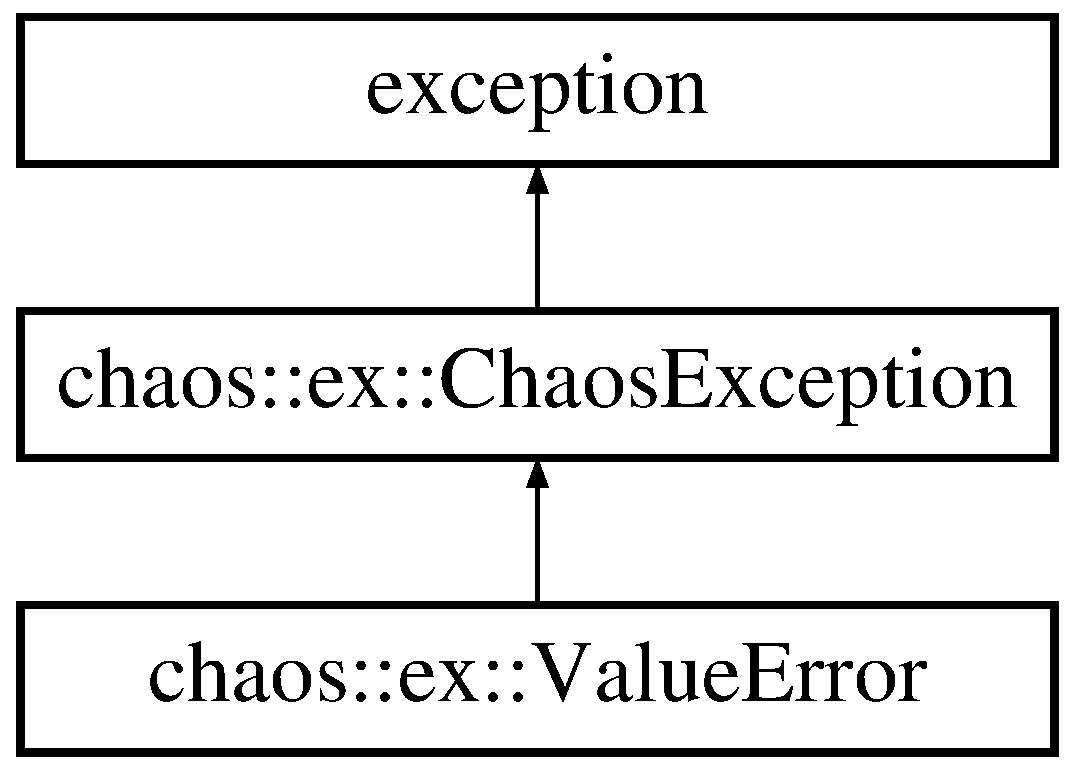
\includegraphics[height=3.000000cm]{classchaos_1_1ex_1_1_value_error}
\end{center}
\end{figure}
\subsection*{Public Member Functions}
\begin{DoxyCompactItemize}
\item 
\hypertarget{classchaos_1_1ex_1_1_value_error_ad7c90b7ae603eec76908add85d311633}{}{\bfseries Value\+Error} (const \hyperlink{classchaos_1_1str_1_1_u_t_f8_string}{chaos\+::str\+::\+U\+T\+F8\+String} \&message)\label{classchaos_1_1ex_1_1_value_error_ad7c90b7ae603eec76908add85d311633}

\end{DoxyCompactItemize}
\subsection*{Additional Inherited Members}


\subsection{Detailed Description}
Warns that an invalid value has been supplied. 

The documentation for this class was generated from the following file\+:\begin{DoxyCompactItemize}
\item 
D\+:/\+Dropbox/\+Development/\+Chaos\+Core/\+Chaos\+Core/src/cxx/chaoscore/base/\hyperlink{_base_exceptions_8hpp}{Base\+Exceptions.\+hpp}\end{DoxyCompactItemize}

\chapter{File Documentation}
\hypertarget{_base_exceptions_8hpp}{\section{/home/david/\-Dropbox/\-Development/\-Chaos\-Core/\-Chaos\-Core/src/cxx/chaoscore/base/\-Base\-Exceptions.hpp File Reference}
\label{_base_exceptions_8hpp}\index{/home/david/\-Dropbox/\-Development/\-Chaos\-Core/\-Chaos\-Core/src/cxx/chaoscore/base/\-Base\-Exceptions.\-hpp@{/home/david/\-Dropbox/\-Development/\-Chaos\-Core/\-Chaos\-Core/src/cxx/chaoscore/base/\-Base\-Exceptions.\-hpp}}
}
{\ttfamily \#include $<$exception$>$}\\*
{\ttfamily \#include \char`\"{}chaoscore/base/string/\-U\-T\-F8\-String.\-hpp\char`\"{}}\\*
\subsection*{Classes}
\begin{DoxyCompactItemize}
\item 
class \hyperlink{classchaos_1_1ex_1_1_chaos_exception}{chaos\-::ex\-::\-Chaos\-Exception}
\begin{DoxyCompactList}\small\item\em Abstract base class that all Chaos\-Core Exceptions extend from. \end{DoxyCompactList}\item 
class \hyperlink{classchaos_1_1ex_1_1_not_implemented_error}{chaos\-::ex\-::\-Not\-Implemented\-Error}
\begin{DoxyCompactList}\small\item\em Warns that an operations has been performed that has not yet been implemented. \end{DoxyCompactList}\item 
class \hyperlink{classchaos_1_1ex_1_1_value_error}{chaos\-::ex\-::\-Value\-Error}
\begin{DoxyCompactList}\small\item\em Warns that an invalid value has been supplied. \end{DoxyCompactList}\item 
class \hyperlink{classchaos_1_1ex_1_1_index_out_of_bounds_error}{chaos\-::ex\-::\-Index\-Out\-Of\-Bounds\-Error}
\begin{DoxyCompactList}\small\item\em Warns that an index has been requested outside of the allowed bounds. \end{DoxyCompactList}\item 
class \hyperlink{classchaos_1_1ex_1_1_conversion_data_error}{chaos\-::ex\-::\-Conversion\-Data\-Error}
\begin{DoxyCompactList}\small\item\em Warns that the provided data for a type conversion was bad or invalid. \end{DoxyCompactList}\end{DoxyCompactItemize}
\subsection*{Namespaces}
\begin{DoxyCompactItemize}
\item 
\hyperlink{namespacechaos}{chaos}
\begin{DoxyCompactList}\small\item\em the global Chaos\-Core namespace which contains everything within Chaos\-Core. \end{DoxyCompactList}\item 
\hyperlink{namespacechaos_1_1ex}{chaos\-::ex}
\begin{DoxyCompactList}\small\item\em Base generic exceptions defined by Chaos\-Core. \end{DoxyCompactList}\end{DoxyCompactItemize}


\subsection{Detailed Description}
\begin{DoxyAuthor}{Author}
David Saxon 
\end{DoxyAuthor}

\hypertarget{_base_literals_8hpp}{}\section{D\+:/\+Dropbox/\+Development/\+Chaos\+Core/\+Chaos\+Core/src/cxx/chaoscore/base/\+Base\+Literals.hpp File Reference}
\label{_base_literals_8hpp}\index{D\+:/\+Dropbox/\+Development/\+Chaos\+Core/\+Chaos\+Core/src/cxx/chaoscore/base/\+Base\+Literals.\+hpp@{D\+:/\+Dropbox/\+Development/\+Chaos\+Core/\+Chaos\+Core/src/cxx/chaoscore/base/\+Base\+Literals.\+hpp}}
{\ttfamily \#include \char`\"{}chaoscore/base/uni/\+U\+T\+F8\+String.\+hpp\char`\"{}}\\*
\subsection*{Namespaces}
\begin{DoxyCompactItemize}
\item 
 \hyperlink{namespacechaos}{chaos}
\begin{DoxyCompactList}\small\item\em the global Chaos\+Core namespace which contains everything within Chaos\+Core. \end{DoxyCompactList}\item 
 \hyperlink{namespacechaos_1_1literal}{chaos\+::literal}
\begin{DoxyCompactList}\small\item\em User defined literal operators for Chaos\+Core. \end{DoxyCompactList}\end{DoxyCompactItemize}
\subsection*{Macros}
\begin{DoxyCompactItemize}
\item 
\hypertarget{_base_literals_8hpp_a21cc48c0fbef54fbfc8220fc9a8f83de}{}\#define {\bfseries C\+H\+A\+O\+S\+\_\+\+B\+A\+S\+E\+\_\+\+U\+S\+E\+\_\+\+L\+I\+T\+E\+R\+A\+L\+S}\label{_base_literals_8hpp_a21cc48c0fbef54fbfc8220fc9a8f83de}

\end{DoxyCompactItemize}
\subsection*{Functions}
\begin{DoxyCompactItemize}
\item 
\hyperlink{classchaos_1_1uni_1_1_u_t_f8_string}{chaos\+::uni\+::\+U\+T\+F8\+String} \hyperlink{namespacechaos_1_1literal_a07ff12ff0e49317fe54b9c14b65e902c}{chaos\+::literal\+::operator\char`\"{}\char`\"{}\+\_\+utf8} (const char $\ast$literal, size\+\_\+t length)
\begin{DoxyCompactList}\small\item\em Creates a chaos\+::\+U\+T\+F8\+String from a cstring literal. \end{DoxyCompactList}\end{DoxyCompactItemize}


\subsection{Detailed Description}
\begin{DoxyAuthor}{Author}
David Saxon 
\end{DoxyAuthor}

\hypertarget{_binary_operations_8hpp}{\section{/home/david/\-Dropbox/\-Development/\-Chaos\-Core/\-Chaos\-Core/src/cxx/chaoscore/base/data/\-Binary\-Operations.hpp File Reference}
\label{_binary_operations_8hpp}\index{/home/david/\-Dropbox/\-Development/\-Chaos\-Core/\-Chaos\-Core/src/cxx/chaoscore/base/data/\-Binary\-Operations.\-hpp@{/home/david/\-Dropbox/\-Development/\-Chaos\-Core/\-Chaos\-Core/src/cxx/chaoscore/base/data/\-Binary\-Operations.\-hpp}}
}


functions for manipulating and reading binary data.  


\subsection*{Namespaces}
\begin{DoxyCompactItemize}
\item 
\hyperlink{namespacechaos}{chaos}
\begin{DoxyCompactList}\small\item\em the global Chaos\-Core namespace which contains everything within Chaos\-Core. \end{DoxyCompactList}\item 
\hyperlink{namespacechaos_1_1data}{chaos\-::data}
\begin{DoxyCompactList}\small\item\em Module for dealing with low-\/level data. \end{DoxyCompactList}\end{DoxyCompactItemize}
\subsection*{Enumerations}
\begin{DoxyCompactItemize}
\item 
enum \hyperlink{namespacechaos_1_1data_adb2657d50c0b84cdc1153001031bbf3f}{chaos\-::data\-::\-Endianness} \{ \hyperlink{namespacechaos_1_1data_adb2657d50c0b84cdc1153001031bbf3fa7fc5455bb6147c278dfa4a84e255c66d}{chaos\-::data\-::\-E\-N\-D\-I\-A\-N\-\_\-\-L\-I\-T\-T\-L\-E}, 
\hyperlink{namespacechaos_1_1data_adb2657d50c0b84cdc1153001031bbf3fa0e1ed99b965cedefe24534be309738ad}{chaos\-::data\-::\-E\-N\-D\-I\-A\-N\-\_\-\-B\-I\-G}
 \}
\begin{DoxyCompactList}\small\item\em The possible endian types. \end{DoxyCompactList}\end{DoxyCompactItemize}
\subsection*{Functions}
\begin{DoxyCompactItemize}
\item 
\hypertarget{namespacechaos_1_1data_a853118d28d026784faad6673bbcf526f}{Endianness \hyperlink{namespacechaos_1_1data_a853118d28d026784faad6673bbcf526f}{chaos\-::data\-::get\-\_\-system\-\_\-endianness} ()}\label{namespacechaos_1_1data_a853118d28d026784faad6673bbcf526f}

\begin{DoxyCompactList}\small\item\em Returns the endianness of the current system this is running on. \end{DoxyCompactList}\end{DoxyCompactItemize}


\subsection{Detailed Description}
functions for manipulating and reading binary data. \begin{DoxyAuthor}{Author}
David Saxon 
\end{DoxyAuthor}

\hypertarget{_byte_operations_8hpp}{}\section{D\+:/\+Dropbox/\+Development/\+Chaos\+Core/\+Chaos\+Core/src/cxx/chaoscore/base/data/\+Byte\+Operations.hpp File Reference}
\label{_byte_operations_8hpp}\index{D\+:/\+Dropbox/\+Development/\+Chaos\+Core/\+Chaos\+Core/src/cxx/chaoscore/base/data/\+Byte\+Operations.\+hpp@{D\+:/\+Dropbox/\+Development/\+Chaos\+Core/\+Chaos\+Core/src/cxx/chaoscore/base/data/\+Byte\+Operations.\+hpp}}


functions for manipulating and reading byte data.  


{\ttfamily \#include $<$cstdlib$>$}\\*
{\ttfamily \#include \char`\"{}chaoscore/base/\+Types.\+hpp\char`\"{}}\\*
{\ttfamily \#include \char`\"{}chaoscore/base/data/\+Binary\+Operations.\+hpp\char`\"{}}\\*
\subsection*{Namespaces}
\begin{DoxyCompactItemize}
\item 
 \hyperlink{namespacechaos}{chaos}
\begin{DoxyCompactList}\small\item\em the global Chaos\+Core namespace which contains everything within Chaos\+Core. \end{DoxyCompactList}\item 
 \hyperlink{namespacechaos_1_1data}{chaos\+::data}
\begin{DoxyCompactList}\small\item\em Module for dealing with low-\/level data. \end{DoxyCompactList}\end{DoxyCompactItemize}
\subsection*{Functions}
\begin{DoxyCompactItemize}
\item 
\hyperlink{namespacechaos_a8641b3ae4551f0b35570d4f9f4ec22d9}{chaos\+::uint32} \hyperlink{namespacechaos_1_1data_af4310ad815f14c278c83c5abb3abc251}{chaos\+::data\+::bytes\+\_\+to\+\_\+uint32} (const void $\ast$bytes, std\+::size\+\_\+t length, Endianness endianness=\hyperlink{namespacechaos_1_1data_a853118d28d026784faad6673bbcf526f}{chaos\+::data\+::get\+\_\+system\+\_\+endianness}())
\begin{DoxyCompactList}\small\item\em Converts an array of bytes to a single unsigned 32-\/bit integer. \end{DoxyCompactList}\end{DoxyCompactItemize}


\subsection{Detailed Description}
functions for manipulating and reading byte data. 

\begin{DoxyAuthor}{Author}
David Saxon 
\end{DoxyAuthor}

\hypertarget{_math_operations_8hpp}{\section{/home/david/\-Dropbox/\-Development/\-Chaos\-Core/\-Chaos\-Core/src/cxx/chaoscore/base/math/\-Math\-Operations.hpp File Reference}
\label{_math_operations_8hpp}\index{/home/david/\-Dropbox/\-Development/\-Chaos\-Core/\-Chaos\-Core/src/cxx/chaoscore/base/math/\-Math\-Operations.\-hpp@{/home/david/\-Dropbox/\-Development/\-Chaos\-Core/\-Chaos\-Core/src/cxx/chaoscore/base/math/\-Math\-Operations.\-hpp}}
}


Operations relating to math.  


{\ttfamily \#include $<$cfloat$>$}\\*
{\ttfamily \#include \char`\"{}chaoscore/base/math/\-Math\-Constants.\-hpp\char`\"{}}\\*
\subsection*{Namespaces}
\begin{DoxyCompactItemize}
\item 
\hyperlink{namespacechaos}{chaos}
\begin{DoxyCompactList}\small\item\em the global Chaos\-Core namespace which contains everything within Chaos\-Core. \end{DoxyCompactList}\item 
\hyperlink{namespacechaos_1_1math}{chaos\-::math}
\begin{DoxyCompactList}\small\item\em Math related classes and operations. \end{DoxyCompactList}\end{DoxyCompactItemize}
\subsection*{Functions}
\begin{DoxyCompactItemize}
\item 
bool \hyperlink{namespacechaos_1_1math_a45b789648ddacd3e1d2403834c1953a6}{chaos\-::math\-::float\-\_\-equals} (float a, float b, float delta\-\_\-threshold=F\-L\-T\-\_\-\-E\-P\-S\-I\-L\-O\-N, \hyperlink{namespacechaos_a8641b3ae4551f0b35570d4f9f4ec22d9}{chaos\-::uint32} ulps\-\_\-threshold=8)
\begin{DoxyCompactList}\small\item\em Checks whether two floating point values are equal or almost equal. \end{DoxyCompactList}\end{DoxyCompactItemize}


\subsection{Detailed Description}
Operations relating to math. \begin{DoxyAuthor}{Author}
David Saxon 
\end{DoxyAuthor}

\hypertarget{_preproc_8hpp}{\section{/home/david/\-Dropbox/\-Development/\-Chaos\-Core/\-Chaos\-Core/src/cxx/chaoscore/base/\-Preproc.hpp File Reference}
\label{_preproc_8hpp}\index{/home/david/\-Dropbox/\-Development/\-Chaos\-Core/\-Chaos\-Core/src/cxx/chaoscore/base/\-Preproc.\-hpp@{/home/david/\-Dropbox/\-Development/\-Chaos\-Core/\-Chaos\-Core/src/cxx/chaoscore/base/\-Preproc.\-hpp}}
}


A collection of general preprocessor directives and macros.  


\subsection*{Macros}
\begin{DoxyCompactItemize}
\item 
\hypertarget{_preproc_8hpp_a3391fa429b57c110dbf3336e41a515fb}{\#define \hyperlink{_preproc_8hpp_a3391fa429b57c110dbf3336e41a515fb}{C\-H\-A\-O\-S\-\_\-\-O\-S\-\_\-\-W\-I\-N\-D\-O\-W\-S}}\label{_preproc_8hpp_a3391fa429b57c110dbf3336e41a515fb}

\begin{DoxyCompactList}\small\item\em Directive that is defined if the current platform is a Windows operating system. \end{DoxyCompactList}\item 
\hypertarget{_preproc_8hpp_aa95ddbdb0bb581ee7b81309c761e039a}{\#define \hyperlink{_preproc_8hpp_aa95ddbdb0bb581ee7b81309c761e039a}{C\-H\-A\-O\-S\-\_\-\-O\-S\-\_\-\-U\-N\-I\-X}}\label{_preproc_8hpp_aa95ddbdb0bb581ee7b81309c761e039a}

\begin{DoxyCompactList}\small\item\em Directive that is defined if the current platform is a Unix based operating system. \end{DoxyCompactList}\item 
\#define \hyperlink{_preproc_8hpp_a499ec11e7bfb5aa8909bb1db17a6dcce}{C\-H\-A\-O\-S\-\_\-\-O\-S\-\_\-\-M\-A\-C}
\begin{DoxyCompactList}\small\item\em Directive that is defined if the current platform is a Mac operating system. \end{DoxyCompactList}\item 
\#define \hyperlink{_preproc_8hpp_ae454b10c5c96b60e15c761fba0d6f28d}{C\-H\-A\-O\-S\-\_\-\-O\-S\-\_\-\-L\-I\-N\-U\-X}
\begin{DoxyCompactList}\small\item\em Directive that is defined if the current platform is a Linux based operating system. \end{DoxyCompactList}\item 
\hypertarget{_preproc_8hpp_ad397cab0ba48918884a517609d66881d}{\#define \hyperlink{_preproc_8hpp_ad397cab0ba48918884a517609d66881d}{C\-H\-A\-O\-S\-\_\-\-O\-S\-\_\-\-U\-N\-K\-N\-O\-W\-N}}\label{_preproc_8hpp_ad397cab0ba48918884a517609d66881d}

\begin{DoxyCompactList}\small\item\em Directive that is defined if the current could not be detected. \end{DoxyCompactList}\item 
\#define \hyperlink{_preproc_8hpp_a1dbb6cf785739a66694541bacde3c348}{C\-H\-A\-O\-S\-\_\-\-D\-I\-S\-A\-L\-L\-O\-W\-\_\-\-C\-O\-N\-S\-T\-R\-U\-C\-T\-I\-O\-N}(Type\-Name)
\begin{DoxyCompactList}\small\item\em Used to disable all construction methods for a class. \end{DoxyCompactList}\item 
\#define \hyperlink{_preproc_8hpp_a0989a3ffc8b50ec7d96bf6cc3f0f41a4}{C\-H\-A\-O\-S\-\_\-\-D\-I\-S\-A\-L\-L\-O\-W\-\_\-\-C\-O\-P\-Y\-\_\-\-A\-N\-D\-\_\-\-A\-S\-S\-I\-G\-N}(Type\-Name)
\begin{DoxyCompactList}\small\item\em Used to disable the copy constructor and assignment operator for a class. \end{DoxyCompactList}\end{DoxyCompactItemize}


\subsection{Detailed Description}
A collection of general preprocessor directives and macros. \begin{DoxyAuthor}{Author}
David Saxon 
\end{DoxyAuthor}


\subsection{Macro Definition Documentation}
\hypertarget{_preproc_8hpp_a1dbb6cf785739a66694541bacde3c348}{\index{Preproc.\-hpp@{Preproc.\-hpp}!C\-H\-A\-O\-S\-\_\-\-D\-I\-S\-A\-L\-L\-O\-W\-\_\-\-C\-O\-N\-S\-T\-R\-U\-C\-T\-I\-O\-N@{C\-H\-A\-O\-S\-\_\-\-D\-I\-S\-A\-L\-L\-O\-W\-\_\-\-C\-O\-N\-S\-T\-R\-U\-C\-T\-I\-O\-N}}
\index{C\-H\-A\-O\-S\-\_\-\-D\-I\-S\-A\-L\-L\-O\-W\-\_\-\-C\-O\-N\-S\-T\-R\-U\-C\-T\-I\-O\-N@{C\-H\-A\-O\-S\-\_\-\-D\-I\-S\-A\-L\-L\-O\-W\-\_\-\-C\-O\-N\-S\-T\-R\-U\-C\-T\-I\-O\-N}!Preproc.hpp@{Preproc.\-hpp}}
\subsubsection[{C\-H\-A\-O\-S\-\_\-\-D\-I\-S\-A\-L\-L\-O\-W\-\_\-\-C\-O\-N\-S\-T\-R\-U\-C\-T\-I\-O\-N}]{\setlength{\rightskip}{0pt plus 5cm}\#define C\-H\-A\-O\-S\-\_\-\-D\-I\-S\-A\-L\-L\-O\-W\-\_\-\-C\-O\-N\-S\-T\-R\-U\-C\-T\-I\-O\-N(
\begin{DoxyParamCaption}
\item[{}]{Type\-Name}
\end{DoxyParamCaption}
)}}\label{_preproc_8hpp_a1dbb6cf785739a66694541bacde3c348}
{\bfseries Value\-:}
\begin{DoxyCode}
TypeName() = \textcolor{keyword}{delete};                    \(\backslash\)
        TypeName( \textcolor{keyword}{const} TypeName& ) = \textcolor{keyword}{delete};   \(\backslash\)
        void operator=( \textcolor{keyword}{const} TypeName& ) = \textcolor{keyword}{delete}
\end{DoxyCode}


Used to disable all construction methods for a class. 

This macro will explicitly delete the default constructor, copy constructor, and the assignment operator. This is normally only needed in rare edge cases for entirely static classes.

To use this macro it must be declared in the base of the desired class and the name of the class must be passed in as Type\-Name. \hypertarget{_preproc_8hpp_a0989a3ffc8b50ec7d96bf6cc3f0f41a4}{\index{Preproc.\-hpp@{Preproc.\-hpp}!C\-H\-A\-O\-S\-\_\-\-D\-I\-S\-A\-L\-L\-O\-W\-\_\-\-C\-O\-P\-Y\-\_\-\-A\-N\-D\-\_\-\-A\-S\-S\-I\-G\-N@{C\-H\-A\-O\-S\-\_\-\-D\-I\-S\-A\-L\-L\-O\-W\-\_\-\-C\-O\-P\-Y\-\_\-\-A\-N\-D\-\_\-\-A\-S\-S\-I\-G\-N}}
\index{C\-H\-A\-O\-S\-\_\-\-D\-I\-S\-A\-L\-L\-O\-W\-\_\-\-C\-O\-P\-Y\-\_\-\-A\-N\-D\-\_\-\-A\-S\-S\-I\-G\-N@{C\-H\-A\-O\-S\-\_\-\-D\-I\-S\-A\-L\-L\-O\-W\-\_\-\-C\-O\-P\-Y\-\_\-\-A\-N\-D\-\_\-\-A\-S\-S\-I\-G\-N}!Preproc.hpp@{Preproc.\-hpp}}
\subsubsection[{C\-H\-A\-O\-S\-\_\-\-D\-I\-S\-A\-L\-L\-O\-W\-\_\-\-C\-O\-P\-Y\-\_\-\-A\-N\-D\-\_\-\-A\-S\-S\-I\-G\-N}]{\setlength{\rightskip}{0pt plus 5cm}\#define C\-H\-A\-O\-S\-\_\-\-D\-I\-S\-A\-L\-L\-O\-W\-\_\-\-C\-O\-P\-Y\-\_\-\-A\-N\-D\-\_\-\-A\-S\-S\-I\-G\-N(
\begin{DoxyParamCaption}
\item[{}]{Type\-Name}
\end{DoxyParamCaption}
)}}\label{_preproc_8hpp_a0989a3ffc8b50ec7d96bf6cc3f0f41a4}
{\bfseries Value\-:}
\begin{DoxyCode}
TypeName( \textcolor{keyword}{const} TypeName& ) = \textcolor{keyword}{delete};      \(\backslash\)
        void operator=( \textcolor{keyword}{const} TypeName& ) = \textcolor{keyword}{delete}
\end{DoxyCode}


Used to disable the copy constructor and assignment operator for a class. 

The purpose of this macro is to define classes that should not be copied. It explicitly deletes the copy constructor and the assignment operator.

To use this macro it must be declared in the base of the desired class and the name of the class must be passed in as Type\-Name. \hypertarget{_preproc_8hpp_ae454b10c5c96b60e15c761fba0d6f28d}{\index{Preproc.\-hpp@{Preproc.\-hpp}!C\-H\-A\-O\-S\-\_\-\-O\-S\-\_\-\-L\-I\-N\-U\-X@{C\-H\-A\-O\-S\-\_\-\-O\-S\-\_\-\-L\-I\-N\-U\-X}}
\index{C\-H\-A\-O\-S\-\_\-\-O\-S\-\_\-\-L\-I\-N\-U\-X@{C\-H\-A\-O\-S\-\_\-\-O\-S\-\_\-\-L\-I\-N\-U\-X}!Preproc.hpp@{Preproc.\-hpp}}
\subsubsection[{C\-H\-A\-O\-S\-\_\-\-O\-S\-\_\-\-L\-I\-N\-U\-X}]{\setlength{\rightskip}{0pt plus 5cm}\#define C\-H\-A\-O\-S\-\_\-\-O\-S\-\_\-\-L\-I\-N\-U\-X}}\label{_preproc_8hpp_ae454b10c5c96b60e15c761fba0d6f28d}


Directive that is defined if the current platform is a Linux based operating system. 

\begin{DoxyNote}{Note}
The C\-H\-A\-O\-S\-\_\-\-O\-S\-\_\-\-U\-N\-I\-X directive will also be defined in this case. 
\end{DoxyNote}
\hypertarget{_preproc_8hpp_a499ec11e7bfb5aa8909bb1db17a6dcce}{\index{Preproc.\-hpp@{Preproc.\-hpp}!C\-H\-A\-O\-S\-\_\-\-O\-S\-\_\-\-M\-A\-C@{C\-H\-A\-O\-S\-\_\-\-O\-S\-\_\-\-M\-A\-C}}
\index{C\-H\-A\-O\-S\-\_\-\-O\-S\-\_\-\-M\-A\-C@{C\-H\-A\-O\-S\-\_\-\-O\-S\-\_\-\-M\-A\-C}!Preproc.hpp@{Preproc.\-hpp}}
\subsubsection[{C\-H\-A\-O\-S\-\_\-\-O\-S\-\_\-\-M\-A\-C}]{\setlength{\rightskip}{0pt plus 5cm}\#define C\-H\-A\-O\-S\-\_\-\-O\-S\-\_\-\-M\-A\-C}}\label{_preproc_8hpp_a499ec11e7bfb5aa8909bb1db17a6dcce}


Directive that is defined if the current platform is a Mac operating system. 

\begin{DoxyNote}{Note}
The C\-H\-A\-O\-S\-\_\-\-O\-S\-\_\-\-U\-N\-I\-X directive will also be defined in this case. 
\end{DoxyNote}

\hypertarget{_unicode_operations_8hpp}{\section{/home/david/\-Dropbox/\-Development/\-Chaos\-Core/\-Chaos\-Core/src/cxx/chaoscore/base/uni/\-Unicode\-Operations.hpp File Reference}
\label{_unicode_operations_8hpp}\index{/home/david/\-Dropbox/\-Development/\-Chaos\-Core/\-Chaos\-Core/src/cxx/chaoscore/base/uni/\-Unicode\-Operations.\-hpp@{/home/david/\-Dropbox/\-Development/\-Chaos\-Core/\-Chaos\-Core/src/cxx/chaoscore/base/uni/\-Unicode\-Operations.\-hpp}}
}


Operations relating to Unicode string data.  


{\ttfamily \#include \char`\"{}chaoscore/base/\-Types.\-hpp\char`\"{}}\\*
{\ttfamily \#include \char`\"{}chaoscore/base/uni/\-U\-T\-F8\-String.\-hpp\char`\"{}}\\*
\subsection*{Namespaces}
\begin{DoxyCompactItemize}
\item 
\hyperlink{namespacechaos}{chaos}
\begin{DoxyCompactList}\small\item\em the global Chaos\-Core namespace which contains everything within Chaos\-Core. \end{DoxyCompactList}\item 
\hyperlink{namespacechaos_1_1uni}{chaos\-::uni}
\begin{DoxyCompactList}\small\item\em Module for Unicode related classes and operations. \end{DoxyCompactList}\end{DoxyCompactItemize}
\subsection*{Functions}
\begin{DoxyCompactItemize}
\item 
bool \hyperlink{namespacechaos_1_1uni_a25a7549a0378aeac227c881220c23640}{chaos\-::uni\-::is\-\_\-digit} (\hyperlink{namespacechaos_a3b3a47ba1e284655bf1a30c441121c60}{chaos\-::uint32} code\-\_\-point)
\begin{DoxyCompactList}\small\item\em Returns whether the given Unicode code point is a digit or not. \end{DoxyCompactList}\item 
char $\ast$ \hyperlink{namespacechaos_1_1uni_aa2ecaabcd23d2df0cddcc6d00a4a3485}{chaos\-::uni\-::utf8\-\_\-to\-\_\-utf16} (const \hyperlink{classchaos_1_1uni_1_1_u_t_f8_string}{chaos\-::uni\-::\-U\-T\-F8\-String} \&data, size\-\_\-t \&r\-\_\-length=dummy)
\begin{DoxyCompactList}\small\item\em Converts the given \hyperlink{classchaos_1_1uni_1_1_u_t_f8_string}{chaos\-::uni\-::\-U\-T\-F8\-String} encoded data to a new c style string of U\-T\-F-\/16 encoded data. \end{DoxyCompactList}\item 
\hyperlink{classchaos_1_1uni_1_1_u_t_f8_string}{chaos\-::uni\-::\-U\-T\-F8\-String} \hyperlink{namespacechaos_1_1uni_ad2a77983423c8b10e2b18cae6f35d329}{chaos\-::uni\-::join} (const std\-::vector$<$ \hyperlink{classchaos_1_1uni_1_1_u_t_f8_string}{chaos\-::uni\-::\-U\-T\-F8\-String} $>$ \&components, const \hyperlink{classchaos_1_1uni_1_1_u_t_f8_string}{chaos\-::uni\-::\-U\-T\-F8\-String} \&separator)
\begin{DoxyCompactList}\small\item\em Joins the given vector into a single \hyperlink{classchaos_1_1uni_1_1_u_t_f8_string}{chaos\-::uni\-::\-U\-T\-F8\-String}. \end{DoxyCompactList}\end{DoxyCompactItemize}


\subsection{Detailed Description}
Operations relating to Unicode string data. \begin{DoxyAuthor}{Author}
David Saxon 
\end{DoxyAuthor}

\hypertarget{_u_t_f8_string_8hpp}{}\section{D\+:/\+Dropbox/\+Development/\+Chaos\+Core/\+Chaos\+Core/src/cxx/chaoscore/base/uni/\+U\+T\+F8\+String.hpp File Reference}
\label{_u_t_f8_string_8hpp}\index{D\+:/\+Dropbox/\+Development/\+Chaos\+Core/\+Chaos\+Core/src/cxx/chaoscore/base/uni/\+U\+T\+F8\+String.\+hpp@{D\+:/\+Dropbox/\+Development/\+Chaos\+Core/\+Chaos\+Core/src/cxx/chaoscore/base/uni/\+U\+T\+F8\+String.\+hpp}}
{\ttfamily \#include $<$ostream$>$}\\*
{\ttfamily \#include $<$string$>$}\\*
{\ttfamily \#include $<$vector$>$}\\*
{\ttfamily \#include \char`\"{}chaoscore/base/\+Types.\+hpp\char`\"{}}\\*
\subsection*{Classes}
\begin{DoxyCompactItemize}
\item 
class \hyperlink{classchaos_1_1uni_1_1_u_t_f8_string}{chaos\+::uni\+::\+U\+T\+F8\+String}
\begin{DoxyCompactList}\small\item\em A string type designed for storing and manipulating U\+T\+F-\/8 encoded text. \end{DoxyCompactList}\end{DoxyCompactItemize}
\subsection*{Namespaces}
\begin{DoxyCompactItemize}
\item 
 \hyperlink{namespacechaos}{chaos}
\begin{DoxyCompactList}\small\item\em the global Chaos\+Core namespace which contains everything within Chaos\+Core. \end{DoxyCompactList}\item 
 \hyperlink{namespacechaos_1_1uni}{chaos\+::uni}
\begin{DoxyCompactList}\small\item\em Module for Unicode related classes and operations. \end{DoxyCompactList}\end{DoxyCompactItemize}
\subsection*{Functions}
\begin{DoxyCompactItemize}
\item 
\hypertarget{namespacechaos_1_1uni_ab20a8223562ec1ee8f663bda07c7a3ad}{}std\+::ostream \& {\bfseries chaos\+::uni\+::operator$<$$<$} (std\+::ostream \&stream, const U\+T\+F8\+String \&s)\label{namespacechaos_1_1uni_ab20a8223562ec1ee8f663bda07c7a3ad}

\end{DoxyCompactItemize}


\subsection{Detailed Description}
\begin{DoxyAuthor}{Author}
David Saxon 
\end{DoxyAuthor}

\hypertarget{_time_operations_8hpp}{\section{/home/david/\-Dropbox/\-Development/\-Chaos\-Core/\-Chaos\-Core/src/cxx/chaoscore/base/time/\-Time\-Operations.hpp File Reference}
\label{_time_operations_8hpp}\index{/home/david/\-Dropbox/\-Development/\-Chaos\-Core/\-Chaos\-Core/src/cxx/chaoscore/base/time/\-Time\-Operations.\-hpp@{/home/david/\-Dropbox/\-Development/\-Chaos\-Core/\-Chaos\-Core/src/cxx/chaoscore/base/time/\-Time\-Operations.\-hpp}}
}


Utility functions relating to time.  


{\ttfamily \#include \char`\"{}chaoscore/base/\-Types.\-hpp\char`\"{}}\\*
\subsection*{Namespaces}
\begin{DoxyCompactItemize}
\item 
\hyperlink{namespacechaos}{chaos}
\begin{DoxyCompactList}\small\item\em the global Chaos\-Core namespace which contains everything within Chaos\-Core. \end{DoxyCompactList}\item 
\hyperlink{namespacechaos_1_1time}{chaos\-::time}
\begin{DoxyCompactList}\small\item\em Operations and classes relating to time. \end{DoxyCompactList}\end{DoxyCompactItemize}
\subsection*{Functions}
\begin{DoxyCompactItemize}
\item 
\hypertarget{namespacechaos_1_1time_aaf97a80d1887b42f7a026d102382d27d}{\hyperlink{namespacechaos_a34fe5f5bfc3ef6d80b5d094ed91b4d6e}{chaos\-::uint64} \hyperlink{namespacechaos_1_1time_aaf97a80d1887b42f7a026d102382d27d}{chaos\-::time\-::get\-\_\-current\-\_\-time} ()}\label{namespacechaos_1_1time_aaf97a80d1887b42f7a026d102382d27d}

\begin{DoxyCompactList}\small\item\em Returns the time pass since epoch in milliseconds. \end{DoxyCompactList}\end{DoxyCompactItemize}


\subsection{Detailed Description}
Utility functions relating to time. \begin{DoxyAuthor}{Author}
David Saxon 
\end{DoxyAuthor}

\hypertarget{_types_8hpp}{\section{/home/david/\-Dropbox/\-Development/\-Chaos\-Core/\-Chaos\-Core/src/cxx/chaoscore/base/\-Types.hpp File Reference}
\label{_types_8hpp}\index{/home/david/\-Dropbox/\-Development/\-Chaos\-Core/\-Chaos\-Core/src/cxx/chaoscore/base/\-Types.\-hpp@{/home/david/\-Dropbox/\-Development/\-Chaos\-Core/\-Chaos\-Core/src/cxx/chaoscore/base/\-Types.\-hpp}}
}


A collection of {\ttfamily typedefs} for primitive types.  


{\ttfamily \#include \char`\"{}chaoscore/base/\-Preproc.\-hpp\char`\"{}}\\*
{\ttfamily \#include $<$inttypes.\-h$>$}\\*
\subsection*{Namespaces}
\begin{DoxyCompactItemize}
\item 
\hyperlink{namespacechaos}{chaos}
\begin{DoxyCompactList}\small\item\em the global Chaos\-Core namespace which contains everything within Chaos\-Core. \end{DoxyCompactList}\end{DoxyCompactItemize}
\subsection*{Typedefs}
\begin{DoxyCompactItemize}
\item 
typedef int8\-\_\-t \hyperlink{namespacechaos_a56015674cfe4ad1fc583c3da6c724d8a}{chaos\-::int8}
\begin{DoxyCompactList}\small\item\em a 8-\/bit signed integer type \end{DoxyCompactList}\item 
typedef uint8\-\_\-t \hyperlink{namespacechaos_a229e18634387996c2712d57f184bf363}{chaos\-::uint8}
\begin{DoxyCompactList}\small\item\em a 8-\/bit unsigned integer type \end{DoxyCompactList}\item 
typedef int16\-\_\-t \hyperlink{namespacechaos_a23112b8188c8a6ad32a86041fb4c088e}{chaos\-::int16}
\begin{DoxyCompactList}\small\item\em a 16-\/bit signed integer type \end{DoxyCompactList}\item 
typedef uint16\-\_\-t \hyperlink{namespacechaos_ac3888b1c9e56da7fbbdb3ab8425b4068}{chaos\-::uint16}
\begin{DoxyCompactList}\small\item\em a 16-\/bit unsigned integer type \end{DoxyCompactList}\item 
typedef int32\-\_\-t \hyperlink{namespacechaos_ad1de7efb430365afd2c9446a0f522a90}{chaos\-::int32}
\begin{DoxyCompactList}\small\item\em a 32-\/bit signed integer type \end{DoxyCompactList}\item 
typedef uint32\-\_\-t \hyperlink{namespacechaos_a3b3a47ba1e284655bf1a30c441121c60}{chaos\-::uint32}
\begin{DoxyCompactList}\small\item\em a 32-\/bit unsigned integer type \end{DoxyCompactList}\item 
typedef int64\-\_\-t \hyperlink{namespacechaos_a46c61f58d99879b936f58234b9a05e0c}{chaos\-::int64}
\begin{DoxyCompactList}\small\item\em a 64-\/bit signed integer type \end{DoxyCompactList}\item 
typedef uint64\-\_\-t \hyperlink{namespacechaos_a34fe5f5bfc3ef6d80b5d094ed91b4d6e}{chaos\-::uint64}
\begin{DoxyCompactList}\small\item\em a 64-\/bit unsigned integer type \end{DoxyCompactList}\end{DoxyCompactItemize}


\subsection{Detailed Description}
A collection of {\ttfamily typedefs} for primitive types. \begin{DoxyAuthor}{Author}
David Saxon 
\end{DoxyAuthor}

\hypertarget{_file_exceptions_8hpp}{}\section{D\+:/\+Dropbox/\+Development/\+Chaos\+Core/\+Chaos\+Core/src/cxx/chaoscore/base/file/\+File\+Exceptions.hpp File Reference}
\label{_file_exceptions_8hpp}\index{D\+:/\+Dropbox/\+Development/\+Chaos\+Core/\+Chaos\+Core/src/cxx/chaoscore/base/file/\+File\+Exceptions.\+hpp@{D\+:/\+Dropbox/\+Development/\+Chaos\+Core/\+Chaos\+Core/src/cxx/chaoscore/base/file/\+File\+Exceptions.\+hpp}}
{\ttfamily \#include \char`\"{}chaoscore/base/\+Base\+Exceptions.\+hpp\char`\"{}}\\*
\subsection*{Classes}
\begin{DoxyCompactItemize}
\item 
class \hyperlink{classchaos_1_1file_1_1ex_1_1_file_system_error}{chaos\+::file\+::ex\+::\+File\+System\+Error}
\begin{DoxyCompactList}\small\item\em A generic error relating to the file system. \end{DoxyCompactList}\item 
class \hyperlink{classchaos_1_1file_1_1ex_1_1_create_directory_error}{chaos\+::file\+::ex\+::\+Create\+Directory\+Error}
\begin{DoxyCompactList}\small\item\em Warns that creating a directory has failed. \end{DoxyCompactList}\item 
class \hyperlink{classchaos_1_1file_1_1ex_1_1_ambiguous_path_error}{chaos\+::file\+::ex\+::\+Ambiguous\+Path\+Error}
\begin{DoxyCompactList}\small\item\em Warns that has a request has been made to create a file or directory that results in a ambiguous file system path. \end{DoxyCompactList}\end{DoxyCompactItemize}
\subsection*{Namespaces}
\begin{DoxyCompactItemize}
\item 
 \hyperlink{namespacechaos}{chaos}
\begin{DoxyCompactList}\small\item\em the global Chaos\+Core namespace which contains everything within Chaos\+Core. \end{DoxyCompactList}\item 
 \hyperlink{namespacechaos_1_1file}{chaos\+::file}
\begin{DoxyCompactList}\small\item\em File\+System related classes and operations. \end{DoxyCompactList}\item 
 \hyperlink{namespacechaos_1_1file_1_1ex}{chaos\+::file\+::ex}
\begin{DoxyCompactList}\small\item\em Exceptions relating to the file system. \end{DoxyCompactList}\end{DoxyCompactItemize}


\subsection{Detailed Description}
\begin{DoxyAuthor}{Author}
David Saxon 
\end{DoxyAuthor}

\hypertarget{_file_operations_8hpp}{\section{/home/david/\-Dropbox/\-Development/\-Chaos\-Core/\-Chaos\-Core/src/cxx/chaoscore/io/file/\-File\-Operations.hpp File Reference}
\label{_file_operations_8hpp}\index{/home/david/\-Dropbox/\-Development/\-Chaos\-Core/\-Chaos\-Core/src/cxx/chaoscore/io/file/\-File\-Operations.\-hpp@{/home/david/\-Dropbox/\-Development/\-Chaos\-Core/\-Chaos\-Core/src/cxx/chaoscore/io/file/\-File\-Operations.\-hpp}}
}


Utility functions relating to the file system.  


{\ttfamily \#include \char`\"{}chaoscore/base/uni/\-U\-T\-F8\-String.\-hpp\char`\"{}}\\*
\subsection*{Namespaces}
\begin{DoxyCompactItemize}
\item 
\hyperlink{namespacechaos}{chaos}
\begin{DoxyCompactList}\small\item\em the global Chaos\-Core namespace which contains everything within Chaos\-Core. \end{DoxyCompactList}\item 
\hyperlink{namespacechaos_1_1io}{chaos\-::io}
\begin{DoxyCompactList}\small\item\em Input/\-Output related classes and operations. \end{DoxyCompactList}\item 
\hyperlink{namespacechaos_1_1io_1_1file}{chaos\-::io\-::file}
\begin{DoxyCompactList}\small\item\em File\-System related classes and operations. \end{DoxyCompactList}\end{DoxyCompactItemize}
\subsection*{Functions}
\begin{DoxyCompactItemize}
\item 
bool \hyperlink{namespacechaos_1_1io_1_1file_a30e2d7207df6af04322b7f9e11674825}{chaos\-::io\-::file\-::exists} (const \hyperlink{classchaos_1_1uni_1_1_u_t_f8_string}{chaos\-::uni\-::\-U\-T\-F8\-String} \&path)
\begin{DoxyCompactList}\small\item\em Checks whether the given path exists on disk. \end{DoxyCompactList}\item 
bool \hyperlink{namespacechaos_1_1io_1_1file_a310de03ae6c868be8379dc49fe45ea4d}{chaos\-::io\-::file\-::is\-\_\-file} (const \hyperlink{classchaos_1_1uni_1_1_u_t_f8_string}{chaos\-::uni\-::\-U\-T\-F8\-String} \&path)
\begin{DoxyCompactList}\small\item\em Returns whether the given path is a file. \end{DoxyCompactList}\item 
bool \hyperlink{namespacechaos_1_1io_1_1file_ad9890ac8b9dcf3c948274222995c3ea0}{chaos\-::io\-::file\-::is\-\_\-directory} (const \hyperlink{classchaos_1_1uni_1_1_u_t_f8_string}{chaos\-::uni\-::\-U\-T\-F8\-String} \&path)
\begin{DoxyCompactList}\small\item\em Returns whether the given path is a directory. \end{DoxyCompactList}\item 
\hypertarget{namespacechaos_1_1io_1_1file_a9d0395c776184dc23973584a80a86d89}{void \hyperlink{namespacechaos_1_1io_1_1file_a9d0395c776184dc23973584a80a86d89}{chaos\-::io\-::file\-::create\-\_\-directory} (const \hyperlink{classchaos_1_1uni_1_1_u_t_f8_string}{chaos\-::uni\-::\-U\-T\-F8\-String} \&path)}\label{namespacechaos_1_1io_1_1file_a9d0395c776184dc23973584a80a86d89}

\begin{DoxyCompactList}\small\item\em Attempts to create the directory with the given path. \end{DoxyCompactList}\item 
void \hyperlink{namespacechaos_1_1io_1_1file_a85365416303132fc0e8691af65fdcf41}{chaos\-::io\-::file\-::validate\-\_\-path} (const \hyperlink{classchaos_1_1uni_1_1_u_t_f8_string}{chaos\-::uni\-::\-U\-T\-F8\-String} \&path)
\begin{DoxyCompactList}\small\item\em Attempts to directories to the given path if they don't exist. \end{DoxyCompactList}\end{DoxyCompactItemize}


\subsection{Detailed Description}
Utility functions relating to the file system. \begin{DoxyAuthor}{Author}
David Saxon 
\end{DoxyAuthor}

\hypertarget{_a_n_s_i_8hpp}{\section{/home/david/\-Dropbox/\-Development/\-Chaos\-Core/\-Chaos\-Core/src/cxx/chaoscore/io/format/\-A\-N\-S\-I.hpp File Reference}
\label{_a_n_s_i_8hpp}\index{/home/david/\-Dropbox/\-Development/\-Chaos\-Core/\-Chaos\-Core/src/cxx/chaoscore/io/format/\-A\-N\-S\-I.\-hpp@{/home/david/\-Dropbox/\-Development/\-Chaos\-Core/\-Chaos\-Core/src/cxx/chaoscore/io/format/\-A\-N\-S\-I.\-hpp}}
}


Operations relating to A\-N\-S\-I codes. author David Saxon.  


{\ttfamily \#include \char`\"{}chaoscore/base/string/\-U\-T\-F8\-String.\-hpp\char`\"{}}\\*
\subsection*{Namespaces}
\begin{DoxyCompactItemize}
\item 
\hyperlink{namespacechaos}{chaos}
\begin{DoxyCompactList}\small\item\em the global Chaos\-Core namespace which contains everything within Chaos\-Core. \end{DoxyCompactList}\item 
\hyperlink{namespacechaos_1_1io}{chaos\-::io}
\begin{DoxyCompactList}\small\item\em Input/\-Output related classes and operations. \end{DoxyCompactList}\item 
\hyperlink{namespacechaos_1_1io_1_1format}{chaos\-::io\-::format}
\begin{DoxyCompactList}\small\item\em Classes and operations related to formatting. \end{DoxyCompactList}\end{DoxyCompactItemize}
\subsection*{Enumerations}
\begin{DoxyCompactItemize}
\item 
enum \hyperlink{namespacechaos_1_1io_1_1format_aa30dcff2478ffc94e33504c8886a5b1a}{chaos\-::io\-::format\-::\-A\-N\-S\-I\-Colour} \{ \\*
{\bfseries A\-N\-S\-I\-\_\-\-F\-G\-\_\-\-D\-E\-F\-A\-U\-L\-T} = 39, 
{\bfseries A\-N\-S\-I\-\_\-\-F\-G\-\_\-\-B\-L\-A\-C\-K} = 30, 
{\bfseries A\-N\-S\-I\-\_\-\-F\-G\-\_\-\-W\-H\-I\-T\-E} = 97, 
{\bfseries A\-N\-S\-I\-\_\-\-F\-G\-\_\-\-R\-E\-D} = 31, 
\\*
{\bfseries A\-N\-S\-I\-\_\-\-F\-G\-\_\-\-G\-R\-E\-E\-N} = 32, 
{\bfseries A\-N\-S\-I\-\_\-\-F\-G\-\_\-\-Y\-E\-L\-L\-O\-W} = 33, 
{\bfseries A\-N\-S\-I\-\_\-\-F\-G\-\_\-\-B\-L\-U\-E} = 34, 
{\bfseries A\-N\-S\-I\-\_\-\-F\-G\-\_\-\-M\-A\-G\-E\-N\-T\-A} = 35, 
\\*
{\bfseries A\-N\-S\-I\-\_\-\-F\-G\-\_\-\-C\-Y\-A\-N} = 36, 
{\bfseries A\-N\-S\-I\-\_\-\-F\-G\-\_\-\-L\-I\-G\-H\-T\-\_\-\-G\-R\-E\-Y} = 37, 
{\bfseries A\-N\-S\-I\-\_\-\-F\-G\-\_\-\-D\-A\-R\-K\-\_\-\-G\-R\-E\-Y} = 90, 
{\bfseries A\-N\-S\-I\-\_\-\-F\-G\-\_\-\-L\-I\-G\-H\-T\-\_\-\-R\-E\-D} = 91, 
\\*
{\bfseries A\-N\-S\-I\-\_\-\-F\-G\-\_\-\-L\-I\-G\-H\-T\-\_\-\-G\-R\-E\-E\-N} = 92, 
{\bfseries A\-N\-S\-I\-\_\-\-F\-G\-\_\-\-L\-I\-G\-H\-T\-\_\-\-Y\-E\-L\-L\-O\-W} = 93, 
{\bfseries A\-N\-S\-I\-\_\-\-F\-G\-\_\-\-L\-I\-G\-H\-T\-\_\-\-B\-L\-U\-E} = 94, 
{\bfseries A\-N\-S\-I\-\_\-\-F\-G\-\_\-\-L\-I\-G\-H\-T\-\_\-\-M\-A\-G\-E\-N\-T\-A} = 95, 
\\*
{\bfseries A\-N\-S\-I\-\_\-\-F\-G\-\_\-\-L\-I\-G\-H\-T\-\_\-\-C\-Y\-A\-N} = 96, 
{\bfseries A\-N\-S\-I\-\_\-\-B\-G\-\_\-\-D\-E\-F\-A\-U\-L\-T} = 49, 
{\bfseries A\-N\-S\-I\-\_\-\-B\-G\-\_\-\-R\-E\-D} = 41, 
{\bfseries A\-N\-S\-I\-\_\-\-B\-G\-\_\-\-G\-R\-E\-E\-N} = 42, 
\\*
{\bfseries A\-N\-S\-I\-\_\-\-B\-G\-\_\-\-B\-L\-U\-E} = 44
 \}
\begin{DoxyCompactList}\small\item\em Enumerator representing the possible unique A\-N\-S\-I escape sequence colours. \end{DoxyCompactList}\item 
enum \hyperlink{namespacechaos_1_1io_1_1format_af01119682ec0bc616b49641e0c2a7ccf}{chaos\-::io\-::format\-::\-A\-N\-S\-I\-Attribute} \{ \\*
\hyperlink{namespacechaos_1_1io_1_1format_af01119682ec0bc616b49641e0c2a7ccfa3154b286513beb167bb516ea15f1cfb5}{chaos\-::io\-::format\-::\-A\-N\-S\-I\-\_\-\-A\-T\-T\-R\-\_\-\-N\-O\-N\-E}, 
\hyperlink{namespacechaos_1_1io_1_1format_af01119682ec0bc616b49641e0c2a7ccfaada31e77e1e80ea78e0cd08a126271b3}{chaos\-::io\-::format\-::\-A\-N\-S\-I\-\_\-\-A\-T\-T\-R\-\_\-\-B\-O\-L\-D}, 
\hyperlink{namespacechaos_1_1io_1_1format_af01119682ec0bc616b49641e0c2a7ccfa2f1d142ccf489cba5710445abd48555f}{chaos\-::io\-::format\-::\-A\-N\-S\-I\-\_\-\-A\-T\-T\-R\-\_\-\-U\-N\-D\-E\-R\-S\-C\-O\-R\-E}, 
\hyperlink{namespacechaos_1_1io_1_1format_af01119682ec0bc616b49641e0c2a7ccfacd3671458d96396a0fec66c993244186}{chaos\-::io\-::format\-::\-A\-N\-S\-I\-\_\-\-A\-T\-T\-R\-\_\-\-B\-L\-I\-N\-K}, 
\\*
\hyperlink{namespacechaos_1_1io_1_1format_af01119682ec0bc616b49641e0c2a7ccfaa7b58f4c0365d47d2bc98a4587521806}{chaos\-::io\-::format\-::\-A\-N\-S\-I\-\_\-\-A\-T\-T\-R\-\_\-\-R\-E\-V\-E\-R\-S\-E}
 \}
\begin{DoxyCompactList}\small\item\em Enumerator representing the possible unique A\-N\-S\-I escape sequence attributes. \end{DoxyCompactList}\end{DoxyCompactItemize}
\subsection*{Functions}
\begin{DoxyCompactItemize}
\item 
void \hyperlink{namespacechaos_1_1io_1_1format_a005869cc85ba6d9b0fcfad31cf56bda7}{chaos\-::io\-::format\-::apply\-\_\-escape\-\_\-sequence} (\hyperlink{classchaos_1_1str_1_1_u_t_f8_string}{chaos\-::str\-::\-U\-T\-F8\-String} \&text, A\-N\-S\-I\-Colour colour, A\-N\-S\-I\-Attribute attribute=A\-N\-S\-I\-\_\-\-A\-T\-T\-R\-\_\-\-N\-O\-N\-E)
\begin{DoxyCompactList}\small\item\em Applies an A\-N\-S\-I escape sequence to the provided text. \end{DoxyCompactList}\end{DoxyCompactItemize}


\subsection{Detailed Description}
Operations relating to A\-N\-S\-I codes. author David Saxon. 
\hypertarget{_format_operations_8hpp}{\section{/home/david/\-Dropbox/\-Development/\-Chaos\-Core/\-Chaos\-Core/src/cxx/chaoscore/io/format/\-Format\-Operations.hpp File Reference}
\label{_format_operations_8hpp}\index{/home/david/\-Dropbox/\-Development/\-Chaos\-Core/\-Chaos\-Core/src/cxx/chaoscore/io/format/\-Format\-Operations.\-hpp@{/home/david/\-Dropbox/\-Development/\-Chaos\-Core/\-Chaos\-Core/src/cxx/chaoscore/io/format/\-Format\-Operations.\-hpp}}
}


Operations relating to string formatting. author David Saxon.  


{\ttfamily \#include \char`\"{}chaoscore/base/string/\-U\-T\-F8\-String.\-hpp\char`\"{}}\\*
\subsection*{Namespaces}
\begin{DoxyCompactItemize}
\item 
\hyperlink{namespacechaos}{chaos}
\begin{DoxyCompactList}\small\item\em the global Chaos\-Core namespace which contains everything within Chaos\-Core. \end{DoxyCompactList}\item 
\hyperlink{namespacechaos_1_1io}{chaos\-::io}
\begin{DoxyCompactList}\small\item\em Input/\-Output related classes and operations. \end{DoxyCompactList}\item 
\hyperlink{namespacechaos_1_1io_1_1format}{chaos\-::io\-::format}
\begin{DoxyCompactList}\small\item\em Classes and operations related to formatting. \end{DoxyCompactList}\end{DoxyCompactItemize}
\subsection*{Functions}
\begin{DoxyCompactItemize}
\item 
void \hyperlink{namespacechaos_1_1io_1_1format_a626396566ef32d2401d4a0e91594a4a2}{chaos\-::io\-::format\-::centre\-\_\-text} (\hyperlink{classchaos_1_1str_1_1_u_t_f8_string}{chaos\-::str\-::\-U\-T\-F8\-String} \&text, const \hyperlink{namespacechaos_a3b3a47ba1e284655bf1a30c441121c60}{chaos\-::uint32} line\-\_\-length, bool trim\-\_\-trailing=false)
\begin{DoxyCompactList}\small\item\em Centres the given text with whitespace on either side so that has a symbol length equal to line\-\_\-length. \end{DoxyCompactList}\end{DoxyCompactItemize}


\subsection{Detailed Description}
Operations relating to string formatting. author David Saxon. 
\hypertarget{_chaos_test_8hpp}{\section{/home/david/\-Dropbox/\-Development/\-Chaos\-Core/\-Chaos\-Core/src/cxx/chaoscore/test/\-Chaos\-Test.hpp File Reference}
\label{_chaos_test_8hpp}\index{/home/david/\-Dropbox/\-Development/\-Chaos\-Core/\-Chaos\-Core/src/cxx/chaoscore/test/\-Chaos\-Test.\-hpp@{/home/david/\-Dropbox/\-Development/\-Chaos\-Core/\-Chaos\-Core/src/cxx/chaoscore/test/\-Chaos\-Test.\-hpp}}
}
{\ttfamily \#include $<$map$>$}\\*
{\ttfamily \#include $<$vector$>$}\\*
{\ttfamily \#include \char`\"{}chaoscore/base/\-Base\-Exceptions.\-hpp\char`\"{}}\\*
{\ttfamily \#include \char`\"{}chaoscore/base/string/\-U\-T\-F8\-String.\-hpp\char`\"{}}\\*
{\ttfamily \#include $<$iostream$>$}\\*
\subsection*{Classes}
\begin{DoxyCompactItemize}
\item 
class \hyperlink{classchaos_1_1test_1_1_fixture}{chaos\-::test\-::\-Fixture}
\begin{DoxyCompactList}\small\item\em T\-O\-D\-O\-: D\-O\-C. \end{DoxyCompactList}\item 
class \hyperlink{classchaos_1_1test_1_1_test_error}{chaos\-::test\-::\-Test\-Error}
\begin{DoxyCompactList}\small\item\em Warns of an unexpected error during testing procedures. \end{DoxyCompactList}\end{DoxyCompactItemize}
\subsection*{Namespaces}
\begin{DoxyCompactItemize}
\item 
\hyperlink{namespacechaos}{chaos}
\begin{DoxyCompactList}\small\item\em the global Chaos\-Core namespace which contains everything within Chaos\-Core. \end{DoxyCompactList}\item 
\hyperlink{namespacechaos_1_1test}{chaos\-::test}
\begin{DoxyCompactList}\small\item\em Chaos\-Core's testing module. \end{DoxyCompactList}\end{DoxyCompactItemize}
\subsection*{Macros}
\begin{DoxyCompactItemize}
\item 
\#define \hyperlink{_chaos_test_8hpp_a99bafb580d6fe2036b9408c25012ffeb}{C\-H\-A\-O\-S\-\_\-\-T\-E\-S\-T\-\_\-\-U\-N\-I\-T}(path)~\hyperlink{_chaos_test_8hpp_aed518d0b99183e38b10a7f9c51304aef}{C\-H\-A\-O\-S\-\_\-\-T\-E\-S\-T\-\_\-\-U\-N\-I\-T\-\_\-\-F\-I\-X\-T\-U\-R\-E}( path, \hyperlink{classchaos_1_1test_1_1_fixture}{chaos\-::test\-::\-Fixture} )
\begin{DoxyCompactList}\small\item\em T\-O\-D\-O\-: D\-O\-C. \end{DoxyCompactList}\item 
\#define \hyperlink{_chaos_test_8hpp_aed518d0b99183e38b10a7f9c51304aef}{C\-H\-A\-O\-S\-\_\-\-T\-E\-S\-T\-\_\-\-U\-N\-I\-T\-\_\-\-F\-I\-X\-T\-U\-R\-E}(path, fixture\-Type)
\begin{DoxyCompactList}\small\item\em T\-O\-D\-O\-: D\-O\-C. \end{DoxyCompactList}\end{DoxyCompactItemize}


\subsection{Detailed Description}
The Chaos\-Core testing module.

\begin{DoxyAuthor}{Author}
David Saxon 
\end{DoxyAuthor}


\subsection{Macro Definition Documentation}
\hypertarget{_chaos_test_8hpp_a99bafb580d6fe2036b9408c25012ffeb}{\index{Chaos\-Test.\-hpp@{Chaos\-Test.\-hpp}!C\-H\-A\-O\-S\-\_\-\-T\-E\-S\-T\-\_\-\-U\-N\-I\-T@{C\-H\-A\-O\-S\-\_\-\-T\-E\-S\-T\-\_\-\-U\-N\-I\-T}}
\index{C\-H\-A\-O\-S\-\_\-\-T\-E\-S\-T\-\_\-\-U\-N\-I\-T@{C\-H\-A\-O\-S\-\_\-\-T\-E\-S\-T\-\_\-\-U\-N\-I\-T}!ChaosTest.hpp@{Chaos\-Test.\-hpp}}
\subsubsection[{C\-H\-A\-O\-S\-\_\-\-T\-E\-S\-T\-\_\-\-U\-N\-I\-T}]{\setlength{\rightskip}{0pt plus 5cm}\#define C\-H\-A\-O\-S\-\_\-\-T\-E\-S\-T\-\_\-\-U\-N\-I\-T(
\begin{DoxyParamCaption}
\item[{}]{path}
\end{DoxyParamCaption}
)~{\bf C\-H\-A\-O\-S\-\_\-\-T\-E\-S\-T\-\_\-\-U\-N\-I\-T\-\_\-\-F\-I\-X\-T\-U\-R\-E}( path, {\bf chaos\-::test\-::\-Fixture} )}}\label{_chaos_test_8hpp_a99bafb580d6fe2036b9408c25012ffeb}


T\-O\-D\-O\-: D\-O\-C. 

T\-O\-D\-O\-: D\-O\-C \hypertarget{_chaos_test_8hpp_aed518d0b99183e38b10a7f9c51304aef}{\index{Chaos\-Test.\-hpp@{Chaos\-Test.\-hpp}!C\-H\-A\-O\-S\-\_\-\-T\-E\-S\-T\-\_\-\-U\-N\-I\-T\-\_\-\-F\-I\-X\-T\-U\-R\-E@{C\-H\-A\-O\-S\-\_\-\-T\-E\-S\-T\-\_\-\-U\-N\-I\-T\-\_\-\-F\-I\-X\-T\-U\-R\-E}}
\index{C\-H\-A\-O\-S\-\_\-\-T\-E\-S\-T\-\_\-\-U\-N\-I\-T\-\_\-\-F\-I\-X\-T\-U\-R\-E@{C\-H\-A\-O\-S\-\_\-\-T\-E\-S\-T\-\_\-\-U\-N\-I\-T\-\_\-\-F\-I\-X\-T\-U\-R\-E}!ChaosTest.hpp@{Chaos\-Test.\-hpp}}
\subsubsection[{C\-H\-A\-O\-S\-\_\-\-T\-E\-S\-T\-\_\-\-U\-N\-I\-T\-\_\-\-F\-I\-X\-T\-U\-R\-E}]{\setlength{\rightskip}{0pt plus 5cm}\#define C\-H\-A\-O\-S\-\_\-\-T\-E\-S\-T\-\_\-\-U\-N\-I\-T\-\_\-\-F\-I\-X\-T\-U\-R\-E(
\begin{DoxyParamCaption}
\item[{}]{path, }
\item[{}]{fixture\-Type}
\end{DoxyParamCaption}
)}}\label{_chaos_test_8hpp_aed518d0b99183e38b10a7f9c51304aef}
{\bfseries Value\-:}
\begin{DoxyCode}
\textcolor{keyword}{namespace }\hyperlink{_preproc_8hpp_a82a12e050037267a2d4015c9b0ee33c8}{CHAOS\_UNIQUE\_NAME}( chaos\_unit\_test )                             \(\backslash\)
    \{                                                                          \(\backslash\)
    struct ThisUnitWrapper : \textcolor{keyword}{public} chaos::test::internal::UnitTest            \(\backslash\)
    \{                                                                          \(\backslash\)
        virtual \textcolor{keywordtype}{void} execute( \hyperlink{classchaos_1_1test_1_1_fixture}{chaos::test::Fixture}& fixture );                 \(\backslash\)
    \};                                                                         \(\backslash\)
    chaos::test::internal::DeclareTest chaos\_declare\_test(                     \(\backslash\)
            #path,                                                             \(\backslash\)
            \textcolor{keyword}{new} ThisUnitWrapper(),                                             \(\backslash\)
            \textcolor{keyword}{new} fixtureType()                                                  \(\backslash\)
    );                                                                         \(\backslash\)
    \}                                                                          \(\backslash\)
    void \hyperlink{_preproc_8hpp_a82a12e050037267a2d4015c9b0ee33c8}{CHAOS\_UNIQUE\_NAME}( chaos\_unit\_test )::ThisUnitWrapper::execute(       \(\backslash\)
            chaos::test::Fixture& fixture )
\end{DoxyCode}


T\-O\-D\-O\-: D\-O\-C. 

T\-O\-D\-O\-: D\-O\-C 
%--- End generated contents ---

% Index
\newpage
\phantomsection
\addcontentsline{toc}{chapter}{Index}
\printindex

\end{document}
